\documentclass[twoside]{book}

% Packages required by doxygen
\usepackage{calc}
\usepackage{doxygen}
\usepackage{graphicx}
\usepackage[utf8]{inputenc}
\usepackage{makeidx}
\usepackage{multicol}
\usepackage{multirow}
\usepackage{textcomp}
\usepackage[table]{xcolor}

% Font selection
\usepackage[T1]{fontenc}
\usepackage{mathptmx}
\usepackage[scaled=.90]{helvet}
\usepackage{courier}
\usepackage{amssymb}
\usepackage{sectsty}
\renewcommand{\familydefault}{\sfdefault}
\allsectionsfont{%
  \fontseries{bc}\selectfont%
  \color{darkgray}%
}
\renewcommand{\DoxyLabelFont}{%
  \fontseries{bc}\selectfont%
  \color{darkgray}%
}

% Page & text layout
\usepackage{geometry}
\geometry{%
  a4paper,%
  top=2.5cm,%
  bottom=2.5cm,%
  left=2.5cm,%
  right=2.5cm%
}
\tolerance=750
\hfuzz=15pt
\hbadness=750
\setlength{\emergencystretch}{15pt}
\setlength{\parindent}{0cm}
\setlength{\parskip}{0.2cm}
\makeatletter
\renewcommand{\paragraph}{%
  \@startsection{paragraph}{4}{0ex}{-1.0ex}{1.0ex}{%
    \normalfont\normalsize\bfseries\SS@parafont%
  }%
}
\renewcommand{\subparagraph}{%
  \@startsection{subparagraph}{5}{0ex}{-1.0ex}{1.0ex}{%
    \normalfont\normalsize\bfseries\SS@subparafont%
  }%
}
\makeatother

% Headers & footers
\usepackage{fancyhdr}
\pagestyle{fancyplain}
\fancyhead[LE]{\fancyplain{}{\bfseries\thepage}}
\fancyhead[CE]{\fancyplain{}{}}
\fancyhead[RE]{\fancyplain{}{\bfseries\leftmark}}
\fancyhead[LO]{\fancyplain{}{\bfseries\rightmark}}
\fancyhead[CO]{\fancyplain{}{}}
\fancyhead[RO]{\fancyplain{}{\bfseries\thepage}}
\fancyfoot[LE]{\fancyplain{}{}}
\fancyfoot[CE]{\fancyplain{}{}}
\fancyfoot[RE]{\fancyplain{}{\bfseries\scriptsize Generated on Wed Dec 3 2014 08\-:20\-:27 for Medical Cyborgs by Doxygen }}
\fancyfoot[LO]{\fancyplain{}{\bfseries\scriptsize Generated on Wed Dec 3 2014 08\-:20\-:27 for Medical Cyborgs by Doxygen }}
\fancyfoot[CO]{\fancyplain{}{}}
\fancyfoot[RO]{\fancyplain{}{}}
\renewcommand{\footrulewidth}{0.4pt}
\renewcommand{\chaptermark}[1]{%
  \markboth{#1}{}%
}
\renewcommand{\sectionmark}[1]{%
  \markright{\thesection\ #1}%
}

% Indices & bibliography
\usepackage{natbib}
\usepackage[titles]{tocloft}
\setcounter{tocdepth}{3}
\setcounter{secnumdepth}{5}
\makeindex

% Hyperlinks (required, but should be loaded last)
\usepackage{ifpdf}
\ifpdf
  \usepackage[pdftex,pagebackref=true]{hyperref}
\else
  \usepackage[ps2pdf,pagebackref=true]{hyperref}
\fi
\hypersetup{%
  colorlinks=true,%
  linkcolor=blue,%
  citecolor=blue,%
  unicode%
}

% Custom commands
\newcommand{\clearemptydoublepage}{%
  \newpage{\pagestyle{empty}\cleardoublepage}%
}


%===== C O N T E N T S =====

\begin{document}

% Titlepage & ToC
\hypersetup{pageanchor=false}
\pagenumbering{roman}
\begin{titlepage}
\vspace*{7cm}
\begin{center}%
{\Large Medical Cyborgs }\\
\vspace*{1cm}
{\large Generated by Doxygen 1.8.5}\\
\vspace*{0.5cm}
{\small Wed Dec 3 2014 08:20:27}\\
\end{center}
\end{titlepage}
\clearemptydoublepage
\tableofcontents
\clearemptydoublepage
\pagenumbering{arabic}
\hypersetup{pageanchor=true}

%--- Begin generated contents ---
\chapter{readme}
\label{md___users_douglas__documents_software__senior__project_ios__medical__cyborgs__medical__cyborgs_readme}
\hypertarget{md___users_douglas__documents_software__senior__project_ios__medical__cyborgs__medical__cyborgs_readme}{}
This is an introduction to the documenation



 
\chapter{Hierarchical Index}
\section{Class Hierarchy}
This inheritance list is sorted roughly, but not completely, alphabetically\-:\begin{DoxyCompactList}
\item \contentsline{section}{Activity\-Monitor\-Select\-V\-C()}{\pageref{category_activity_monitor_select_v_c_07_08}}{}
\item \contentsline{section}{App\-Delegate()}{\pageref{category_app_delegate_07_08}}{}
\item $<$C\-B\-Central\-Manager\-Delegate$>$\begin{DoxyCompactList}
\item \contentsline{section}{B\-T\-Device\-Manager}{\pageref{interface_b_t_device_manager}}{}
\end{DoxyCompactList}
\item $<$C\-B\-Peripheral\-Delegate$>$\begin{DoxyCompactList}
\item \contentsline{section}{$<$Device\-Common\-Info\-Interface$>$}{\pageref{protocol_device_common_info_interface-p}}{}
\begin{DoxyCompactList}
\item \contentsline{section}{Fit\-Bit\-Flex}{\pageref{interface_fit_bit_flex}}{}
\item \contentsline{section}{Jawbone\-U\-P24}{\pageref{interface_jawbone_u_p24}}{}
\item \contentsline{section}{Mio\-Global\-Link}{\pageref{interface_mio_global_link}}{}
\item \contentsline{section}{Polar\-H7}{\pageref{interface_polar_h7}}{}
\item \contentsline{section}{Wahoo\-Tickr\-X}{\pageref{interface_wahoo_tickr_x}}{}
\end{DoxyCompactList}
\end{DoxyCompactList}
\item $<$C\-L\-Location\-Manager\-Delegate$>$\begin{DoxyCompactList}
\item \contentsline{section}{Device\-Poll\-Manager}{\pageref{interface_device_poll_manager}}{}
\end{DoxyCompactList}
\item \contentsline{section}{Device\-Constants\-And\-Static\-Functions}{\pageref{class_device_constants_and_static_functions}}{}
\item \contentsline{section}{Graph\-V\-C()}{\pageref{category_graph_v_c_07_08}}{}
\item \contentsline{section}{Heart\-Monitor\-Select\-V\-C()}{\pageref{category_heart_monitor_select_v_c_07_08}}{}
\item \contentsline{section}{Home\-Screen\-V\-C()}{\pageref{category_home_screen_v_c_07_08}}{}
\item N\-S\-Object\begin{DoxyCompactList}
\item \contentsline{section}{Background\-Scheduler}{\pageref{interface_background_scheduler}}{}
\item \contentsline{section}{B\-T\-Device\-Manager}{\pageref{interface_b_t_device_manager}}{}
\item \contentsline{section}{D\-B\-Manager}{\pageref{interface_d_b_manager}}{}
\item \contentsline{section}{Device\-Poll\-Manager}{\pageref{interface_device_poll_manager}}{}
\item \contentsline{section}{Fit\-Bit\-Flex}{\pageref{interface_fit_bit_flex}}{}
\item \contentsline{section}{Jawbone\-U\-P24}{\pageref{interface_jawbone_u_p24}}{}
\item \contentsline{section}{Local\-D\-B\-Result}{\pageref{interface_local_d_b_result}}{}
\item \contentsline{section}{Mio\-Global\-Link}{\pageref{interface_mio_global_link}}{}
\item \contentsline{section}{Monitor\-Creation\-Factory}{\pageref{interface_monitor_creation_factory}}{}
\item \contentsline{section}{Personal\-Info}{\pageref{interface_personal_info}}{}
\item \contentsline{section}{Polar\-H7}{\pageref{interface_polar_h7}}{}
\item \contentsline{section}{Remote\-D\-B\-Connection\-Manager}{\pageref{interface_remote_d_b_connection_manager}}{}
\item \contentsline{section}{Wahoo\-Tickr\-X}{\pageref{interface_wahoo_tickr_x}}{}
\end{DoxyCompactList}
\item $<$N\-S\-Object$>$\begin{DoxyCompactList}
\item \contentsline{section}{$<$Activity\-Monitor\-Protocol$>$}{\pageref{protocol_activity_monitor_protocol-p}}{}
\begin{DoxyCompactList}
\item \contentsline{section}{Fit\-Bit\-Flex}{\pageref{interface_fit_bit_flex}}{}
\item \contentsline{section}{Jawbone\-U\-P24}{\pageref{interface_jawbone_u_p24}}{}
\end{DoxyCompactList}
\item \contentsline{section}{$<$B\-T\-Device\-Manager\-Delegate$>$}{\pageref{protocol_b_t_device_manager_delegate-p}}{}
\begin{DoxyCompactList}
\item \contentsline{section}{Device\-Poll\-Manager}{\pageref{interface_device_poll_manager}}{}
\end{DoxyCompactList}
\item \contentsline{section}{$<$Heart\-Monitor\-Protocol$>$}{\pageref{protocol_heart_monitor_protocol-p}}{}
\begin{DoxyCompactList}
\item \contentsline{section}{Mio\-Global\-Link}{\pageref{interface_mio_global_link}}{}
\item \contentsline{section}{Polar\-H7}{\pageref{interface_polar_h7}}{}
\item \contentsline{section}{Wahoo\-Tickr\-X}{\pageref{interface_wahoo_tickr_x}}{}
\end{DoxyCompactList}
\end{DoxyCompactList}
\item $<$N\-S\-U\-R\-L\-Connection\-Data\-Delegate$>$\begin{DoxyCompactList}
\item \contentsline{section}{Patient\-Information\-V\-C}{\pageref{interface_patient_information_v_c}}{}
\end{DoxyCompactList}
\item $<$N\-S\-U\-R\-L\-Connection\-Delegate$>$\begin{DoxyCompactList}
\item \contentsline{section}{Patient\-Information\-V\-C}{\pageref{interface_patient_information_v_c}}{}
\item \contentsline{section}{Remote\-D\-B\-Connection\-Manager}{\pageref{interface_remote_d_b_connection_manager}}{}
\end{DoxyCompactList}
\item \contentsline{section}{Patient\-Information\-V\-C()}{\pageref{category_patient_information_v_c_07_08}}{}
\item \contentsline{section}{Table\-V\-C\-With\-Sounds()}{\pageref{category_table_v_c_with_sounds_07_08}}{}
\item $<$U\-I\-Application\-Delegate$>$\begin{DoxyCompactList}
\item \contentsline{section}{App\-Delegate}{\pageref{interface_app_delegate}}{}
\end{DoxyCompactList}
\item U\-I\-Responder\begin{DoxyCompactList}
\item \contentsline{section}{App\-Delegate}{\pageref{interface_app_delegate}}{}
\end{DoxyCompactList}
\item U\-I\-Table\-View\-Controller\begin{DoxyCompactList}
\item \contentsline{section}{Table\-V\-C\-With\-Sounds}{\pageref{interface_table_v_c_with_sounds}}{}
\begin{DoxyCompactList}
\item \contentsline{section}{Activity\-Monitor\-Select\-V\-C}{\pageref{interface_activity_monitor_select_v_c}}{}
\item \contentsline{section}{Heart\-Monitor\-Select\-V\-C}{\pageref{interface_heart_monitor_select_v_c}}{}
\end{DoxyCompactList}
\end{DoxyCompactList}
\item $<$U\-I\-Text\-Field\-Delegate$>$\begin{DoxyCompactList}
\item \contentsline{section}{Patient\-Information\-V\-C}{\pageref{interface_patient_information_v_c}}{}
\end{DoxyCompactList}
\item U\-I\-View\-Controller\begin{DoxyCompactList}
\item \contentsline{section}{Graph\-V\-C}{\pageref{interface_graph_v_c}}{}
\item \contentsline{section}{Home\-Screen\-V\-C}{\pageref{interface_home_screen_v_c}}{}
\item \contentsline{section}{Patient\-Information\-V\-C}{\pageref{interface_patient_information_v_c}}{}
\end{DoxyCompactList}
\end{DoxyCompactList}

\chapter{Class Index}
\section{Class List}
Here are the classes, structs, unions and interfaces with brief descriptions\-:\begin{DoxyCompactList}
\item\contentsline{section}{\hyperlink{protocol_activity_monitor_protocol-p}{$<$\-Activity\-Monitor\-Protocol$>$} }{\pageref{protocol_activity_monitor_protocol-p}}{}
\item\contentsline{section}{\hyperlink{interface_activity_monitor_select_v_c}{Activity\-Monitor\-Select\-V\-C} }{\pageref{interface_activity_monitor_select_v_c}}{}
\item\contentsline{section}{\hyperlink{category_activity_monitor_select_v_c_07_08}{Activity\-Monitor\-Select\-V\-C()} }{\pageref{category_activity_monitor_select_v_c_07_08}}{}
\item\contentsline{section}{\hyperlink{interface_app_delegate}{App\-Delegate} }{\pageref{interface_app_delegate}}{}
\item\contentsline{section}{\hyperlink{category_app_delegate_07_08}{App\-Delegate()} }{\pageref{category_app_delegate_07_08}}{}
\item\contentsline{section}{\hyperlink{interface_background_scheduler}{Background\-Scheduler} }{\pageref{interface_background_scheduler}}{}
\item\contentsline{section}{\hyperlink{interface_b_t_device_manager}{B\-T\-Device\-Manager} }{\pageref{interface_b_t_device_manager}}{}
\item\contentsline{section}{\hyperlink{protocol_b_t_device_manager_delegate-p}{$<$\-B\-T\-Device\-Manager\-Delegate$>$} }{\pageref{protocol_b_t_device_manager_delegate-p}}{}
\item\contentsline{section}{\hyperlink{interface_d_b_manager}{D\-B\-Manager} }{\pageref{interface_d_b_manager}}{}
\item\contentsline{section}{\hyperlink{protocol_device_common_info_interface-p}{$<$\-Device\-Common\-Info\-Interface$>$} }{\pageref{protocol_device_common_info_interface-p}}{}
\item\contentsline{section}{\hyperlink{class_device_constants_and_static_functions}{Device\-Constants\-And\-Static\-Functions} }{\pageref{class_device_constants_and_static_functions}}{}
\item\contentsline{section}{\hyperlink{interface_device_poll_manager}{Device\-Poll\-Manager} }{\pageref{interface_device_poll_manager}}{}
\item\contentsline{section}{\hyperlink{interface_fit_bit_flex}{Fit\-Bit\-Flex} }{\pageref{interface_fit_bit_flex}}{}
\item\contentsline{section}{\hyperlink{interface_graph_v_c}{Graph\-V\-C} }{\pageref{interface_graph_v_c}}{}
\item\contentsline{section}{\hyperlink{category_graph_v_c_07_08}{Graph\-V\-C()} }{\pageref{category_graph_v_c_07_08}}{}
\item\contentsline{section}{\hyperlink{protocol_heart_monitor_protocol-p}{$<$\-Heart\-Monitor\-Protocol$>$} }{\pageref{protocol_heart_monitor_protocol-p}}{}
\item\contentsline{section}{\hyperlink{interface_heart_monitor_select_v_c}{Heart\-Monitor\-Select\-V\-C} }{\pageref{interface_heart_monitor_select_v_c}}{}
\item\contentsline{section}{\hyperlink{category_heart_monitor_select_v_c_07_08}{Heart\-Monitor\-Select\-V\-C()} }{\pageref{category_heart_monitor_select_v_c_07_08}}{}
\item\contentsline{section}{\hyperlink{interface_home_screen_v_c}{Home\-Screen\-V\-C} }{\pageref{interface_home_screen_v_c}}{}
\item\contentsline{section}{\hyperlink{category_home_screen_v_c_07_08}{Home\-Screen\-V\-C()} }{\pageref{category_home_screen_v_c_07_08}}{}
\item\contentsline{section}{\hyperlink{interface_local_d_b_result}{Local\-D\-B\-Result} }{\pageref{interface_local_d_b_result}}{}
\item\contentsline{section}{\hyperlink{interface_mio_global_link}{Mio\-Global\-Link} }{\pageref{interface_mio_global_link}}{}
\item\contentsline{section}{\hyperlink{interface_monitor_creation_factory}{Monitor\-Creation\-Factory} }{\pageref{interface_monitor_creation_factory}}{}
\item\contentsline{section}{\hyperlink{interface_patient_information_v_c}{Patient\-Information\-V\-C} }{\pageref{interface_patient_information_v_c}}{}
\item\contentsline{section}{\hyperlink{category_patient_information_v_c_07_08}{Patient\-Information\-V\-C()} }{\pageref{category_patient_information_v_c_07_08}}{}
\item\contentsline{section}{\hyperlink{interface_personal_info}{Personal\-Info} }{\pageref{interface_personal_info}}{}
\item\contentsline{section}{\hyperlink{interface_polar_h7}{Polar\-H7} }{\pageref{interface_polar_h7}}{}
\item\contentsline{section}{\hyperlink{interface_remote_d_b_connection_manager}{Remote\-D\-B\-Connection\-Manager} }{\pageref{interface_remote_d_b_connection_manager}}{}
\item\contentsline{section}{\hyperlink{interface_table_v_c_with_sounds}{Table\-V\-C\-With\-Sounds} }{\pageref{interface_table_v_c_with_sounds}}{}
\item\contentsline{section}{\hyperlink{category_table_v_c_with_sounds_07_08}{Table\-V\-C\-With\-Sounds()} }{\pageref{category_table_v_c_with_sounds_07_08}}{}
\item\contentsline{section}{\hyperlink{interface_wahoo_tickr_x}{Wahoo\-Tickr\-X} }{\pageref{interface_wahoo_tickr_x}}{}
\end{DoxyCompactList}

\chapter{Class Documentation}
\hypertarget{protocol_activity_monitor_protocol-p}{\section{$<$Activity\-Monitor\-Protocol$>$ Protocol Reference}
\label{protocol_activity_monitor_protocol-p}\index{$<$\-Activity\-Monitor\-Protocol$>$@{$<$\-Activity\-Monitor\-Protocol$>$}}
}


{\ttfamily \#import $<$Activity\-Monitor\-Protocol.\-h$>$}

Inheritance diagram for $<$Activity\-Monitor\-Protocol$>$\-:\begin{figure}[H]
\begin{center}
\leavevmode
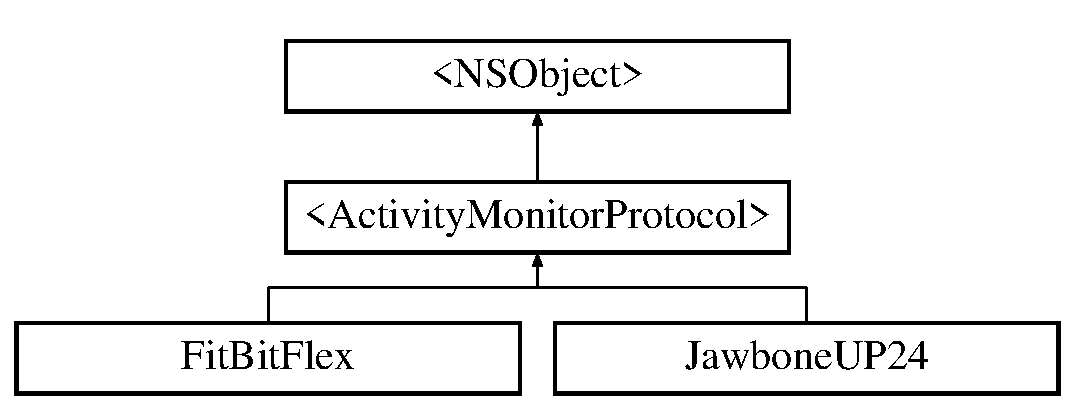
\includegraphics[height=3.000000cm]{protocol_activity_monitor_protocol-p}
\end{center}
\end{figure}
\subsection*{Instance Methods}
\begin{DoxyCompactItemize}
\item 
(N\-S\-Integer) -\/ \hyperlink{protocol_activity_monitor_protocol-p_a3c4e5219c201426d8c1bffa0856a4e3c}{get\-Activity\-Level}
\end{DoxyCompactItemize}


\subsection{Detailed Description}
This protocol is designed to be used on all activity monitor devices. The methods enclosed ensure uniform operation with the application, irrespective of the specific device. It is used for polling so that all modifications are to the specific device and do not have cascading effects to the other devices. 

\subsection{Method Documentation}
\hypertarget{protocol_activity_monitor_protocol-p_a3c4e5219c201426d8c1bffa0856a4e3c}{\index{Activity\-Monitor\-Protocol-\/p@{Activity\-Monitor\-Protocol-\/p}!get\-Activity\-Level@{get\-Activity\-Level}}
\index{get\-Activity\-Level@{get\-Activity\-Level}!ActivityMonitorProtocol-p@{Activity\-Monitor\-Protocol-\/p}}
\subsubsection[{get\-Activity\-Level}]{\setlength{\rightskip}{0pt plus 5cm}-\/ (N\-S\-Integer) get\-Activity\-Level 
\begin{DoxyParamCaption}
{}
\end{DoxyParamCaption}
}}\label{protocol_activity_monitor_protocol-p_a3c4e5219c201426d8c1bffa0856a4e3c}
This methods get an activity level. The result is defined in the \hyperlink{_device_types_8h_source}{Device\-Types.\-h} file.

\begin{DoxyReturn}{Returns}
An integer value that corresponds with the activity level constants in \hyperlink{_device_types_8h_source}{Device\-Types.\-h} 
\end{DoxyReturn}


The documentation for this protocol was generated from the following file\-:\begin{DoxyCompactItemize}
\item 
Activity\-Monitor\-Protocol.\-h\end{DoxyCompactItemize}

\hypertarget{interface_activity_monitor_select_v_c}{\section{Activity\-Monitor\-Select\-V\-C Class Reference}
\label{interface_activity_monitor_select_v_c}\index{Activity\-Monitor\-Select\-V\-C@{Activity\-Monitor\-Select\-V\-C}}
}


{\ttfamily \#import $<$Activity\-Monitor\-Select\-V\-C.\-h$>$}

Inheritance diagram for Activity\-Monitor\-Select\-V\-C\-:\begin{figure}[H]
\begin{center}
\leavevmode
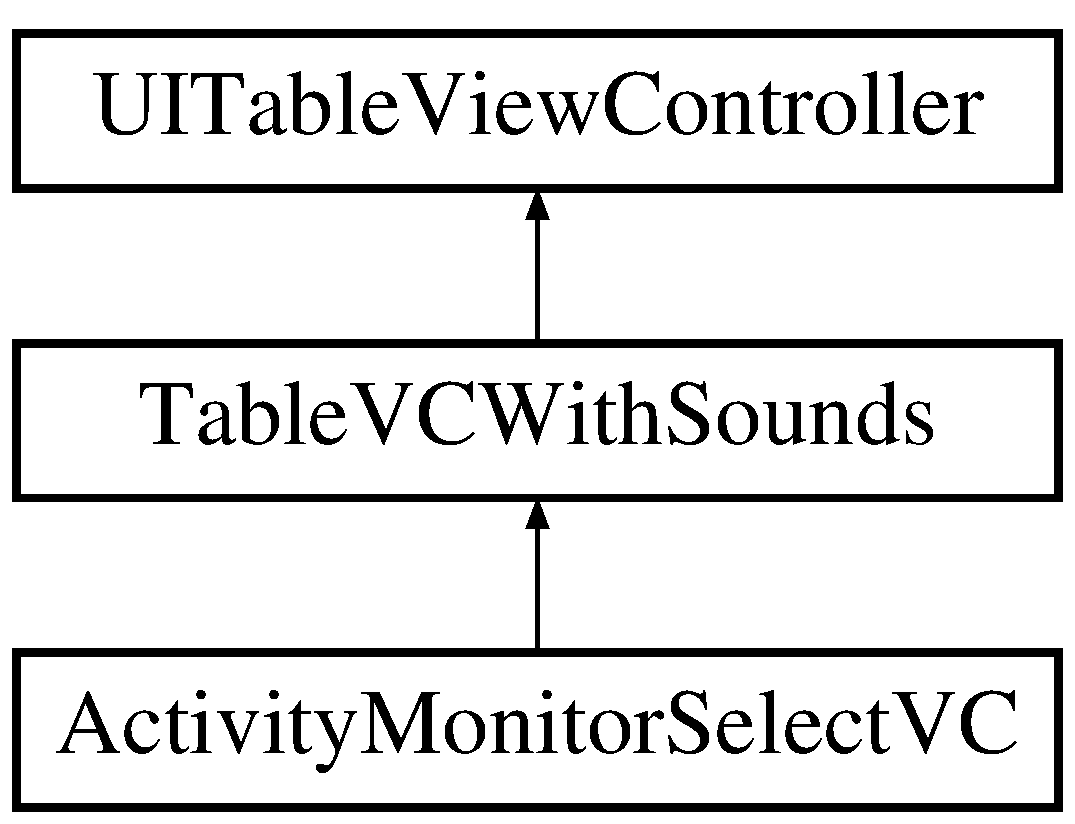
\includegraphics[height=3.000000cm]{interface_activity_monitor_select_v_c}
\end{center}
\end{figure}
\subsection*{Additional Inherited Members}


\subsection{Detailed Description}
This screen allows for selection and discovery of bluetooth devices that conform to the activity monitoring services. 

The documentation for this class was generated from the following file\-:\begin{DoxyCompactItemize}
\item 
/\-Users/douglas/\-Documents/software/\-Senior Project/ios/\-Medical Cyborgs/\-Medical Cyborgs/Activity\-Monitor\-Select\-V\-C.\-h\end{DoxyCompactItemize}

\hypertarget{category_activity_monitor_select_v_c_07_08}{\section{Activity\-Monitor\-Select\-V\-C() Category Reference}
\label{category_activity_monitor_select_v_c_07_08}\index{Activity\-Monitor\-Select\-V\-C()@{Activity\-Monitor\-Select\-V\-C()}}
}


The documentation for this category was generated from the following file\-:\begin{DoxyCompactItemize}
\item 
Activity\-Monitor\-Select\-V\-C.\-m\end{DoxyCompactItemize}

\hypertarget{interface_app_delegate}{\section{App\-Delegate Class Reference}
\label{interface_app_delegate}\index{App\-Delegate@{App\-Delegate}}
}
Inheritance diagram for App\-Delegate\-:\begin{figure}[H]
\begin{center}
\leavevmode
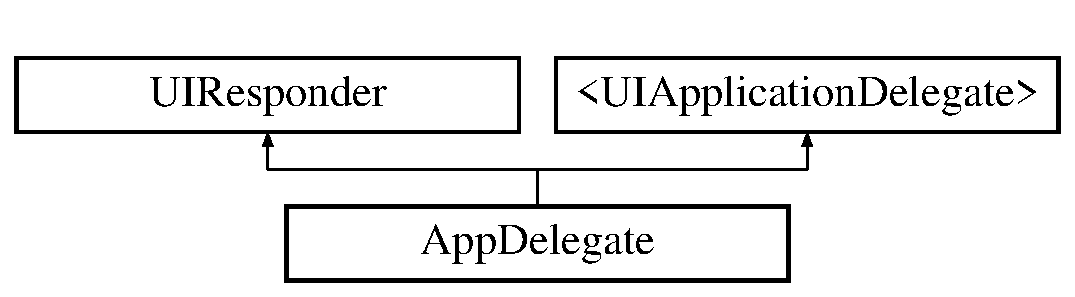
\includegraphics[height=2.000000cm]{interface_app_delegate}
\end{center}
\end{figure}
\subsection*{Properties}
\begin{DoxyCompactItemize}
\item 
\hypertarget{interface_app_delegate_acf48ac24125e688cac1a85445cd7fac2}{U\-I\-Window $\ast$ {\bfseries window}}\label{interface_app_delegate_acf48ac24125e688cac1a85445cd7fac2}

\item 
\hypertarget{interface_app_delegate_a7774bb6fd8b636a6d6b15f91f2809a91}{\hyperlink{interface_background_scheduler}{Background\-Scheduler} $\ast$ {\bfseries process\-Scheduler}}\label{interface_app_delegate_a7774bb6fd8b636a6d6b15f91f2809a91}

\item 
\hypertarget{interface_app_delegate_a22a5a481802e14bae7bd6cbffd141c65}{\hyperlink{interface_home_screen_v_c}{Home\-Screen\-V\-C} $\ast$ {\bfseries home\-Screen}}\label{interface_app_delegate_a22a5a481802e14bae7bd6cbffd141c65}

\end{DoxyCompactItemize}


The documentation for this class was generated from the following file\-:\begin{DoxyCompactItemize}
\item 
/\-Users/douglas/\-Documents/software/\-Senior Project/ios/\-Medical Cyborgs/\-Medical Cyborgs/App\-Delegate.\-h\end{DoxyCompactItemize}

\hypertarget{category_app_delegate_07_08}{\section{App\-Delegate() Category Reference}
\label{category_app_delegate_07_08}\index{App\-Delegate()@{App\-Delegate()}}
}


The documentation for this category was generated from the following file\-:\begin{DoxyCompactItemize}
\item 
App\-Delegate.\-m\end{DoxyCompactItemize}

\hypertarget{interface_background_scheduler}{\section{Background\-Scheduler Class Reference}
\label{interface_background_scheduler}\index{Background\-Scheduler@{Background\-Scheduler}}
}


{\ttfamily \#import $<$Back\-Ground\-Scheduler.\-h$>$}

Inheritance diagram for Background\-Scheduler\-:\begin{figure}[H]
\begin{center}
\leavevmode
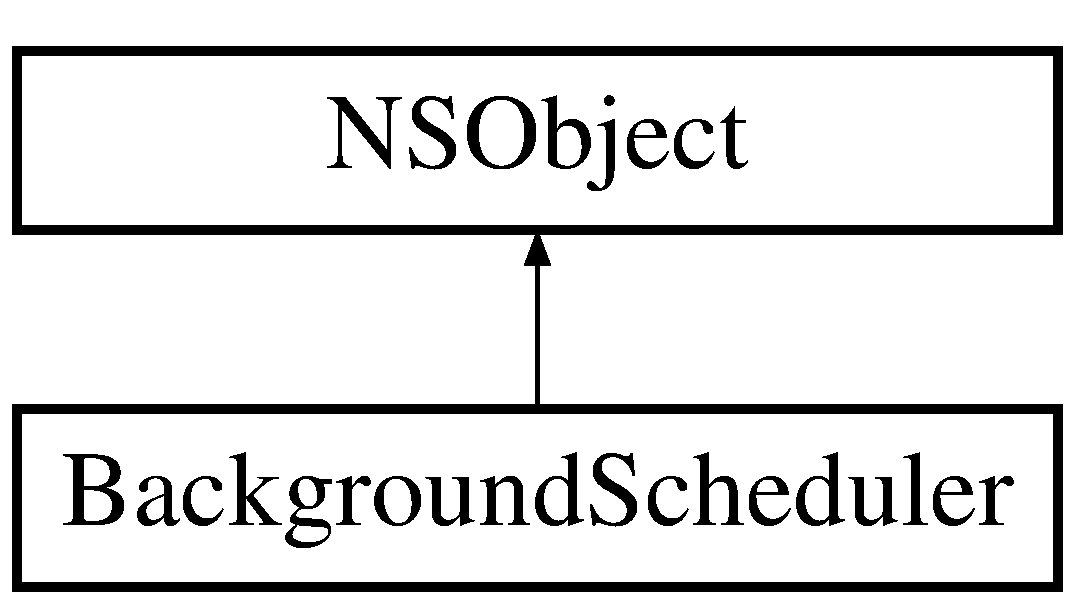
\includegraphics[height=2.000000cm]{interface_background_scheduler}
\end{center}
\end{figure}
\subsection*{Instance Methods}
\begin{DoxyCompactItemize}
\item 
(void) -\/ \hyperlink{interface_background_scheduler_a50173200d1b7dfc44b1d2d2a49ca75be}{start\-Monitoring\-With\-Patient\-I\-D\-:}
\item 
(void) -\/ \hyperlink{interface_background_scheduler_afa9c1aaf67ac8d9f5fd17a43475777eb}{stop\-Monitoring}
\item 
(void) -\/ \hyperlink{interface_background_scheduler_a11390d5d6bb62b2c565ca9205d045b2a}{perform\-Scan}
\item 
(U\-I\-Application $\ast$) -\/ \hyperlink{interface_background_scheduler_a393315828a032dece36a93c53ee203d0}{app}
\end{DoxyCompactItemize}
\subsection*{Properties}
\begin{DoxyCompactItemize}
\item 
\hyperlink{interface_b_t_device_manager}{B\-T\-Device\-Manager} $\ast$ \hyperlink{interface_background_scheduler_aea6a288ffb185db815ddaeaf58c2edcd}{device\-Manager}
\item 
\hyperlink{interface_remote_d_b_connection_manager}{Remote\-D\-B\-Connection\-Manager} $\ast$ \hyperlink{interface_background_scheduler_a6dd785826954ce8d6adc2ad76284c458}{server\-Poller}
\item 
\hyperlink{interface_device_poll_manager}{Device\-Poll\-Manager} $\ast$ \hyperlink{interface_background_scheduler_a9f8103a5d35ba76fd32b5f0d3a2d5517}{device\-Poller}
\item 
\hyperlink{interface_d_b_manager}{D\-B\-Manager} $\ast$ \hyperlink{interface_background_scheduler_a6cacd8a0d6d25475816490b39dcf35d3}{database}
\item 
\hyperlink{interface_personal_info}{Personal\-Info} $\ast$ \hyperlink{interface_background_scheduler_a3f2d5c8d892ff5c8155305ae6bc2da1a}{patient}
\item 
B\-O\-O\-L \hyperlink{interface_background_scheduler_a5209bb2a1aa5fe8eeac8f89977252df7}{allow\-Monitoring}
\item 
N\-S\-Run\-Loop $\ast$ \hyperlink{interface_background_scheduler_a73f120ac0977837ac4a4095ad96d01ec}{run\-Loop}
\item 
N\-S\-Time\-Interval \hyperlink{interface_background_scheduler_ae2e25ad686446576c71a500b66f31e25}{device\-Poll\-Interval}
\item 
N\-S\-Time\-Interval \hyperlink{interface_background_scheduler_a6a4ebd391d86c9779122136b6c4dfc1c}{server\-Poll\-Interval}
\item 
U\-I\-Application $\ast$ \hyperlink{interface_background_scheduler_a8c133b6375de7c3e0cda3ac605ad2029}{app}
\item 
N\-S\-Timer $\ast$ \hyperlink{interface_background_scheduler_a9dee3016296e3a529451c25b426b8923}{device\-Poll\-Timer}
\item 
N\-S\-Timer $\ast$ \hyperlink{interface_background_scheduler_ab78e335cbdbd2c276c299380a982f0e4}{server\-Poll\-Timer}
\end{DoxyCompactItemize}


\subsection{Detailed Description}
This object is responsible for the coordination of the device poller, the database manager, and the process that pushes data to the remote server. 

\subsection{Method Documentation}
\hypertarget{interface_background_scheduler_a393315828a032dece36a93c53ee203d0}{\index{Background\-Scheduler@{Background\-Scheduler}!app@{app}}
\index{app@{app}!BackgroundScheduler@{Background\-Scheduler}}
\subsubsection[{app}]{\setlength{\rightskip}{0pt plus 5cm}-\/ (U\-I\-Application$\ast$) app 
\begin{DoxyParamCaption}
{}
\end{DoxyParamCaption}
}}\label{interface_background_scheduler_a393315828a032dece36a93c53ee203d0}
This method returns the shared instance of the U\-I\-Application. It is placed here to make dependency more obvious. \hypertarget{interface_background_scheduler_a11390d5d6bb62b2c565ca9205d045b2a}{\index{Background\-Scheduler@{Background\-Scheduler}!perform\-Scan@{perform\-Scan}}
\index{perform\-Scan@{perform\-Scan}!BackgroundScheduler@{Background\-Scheduler}}
\subsubsection[{perform\-Scan}]{\setlength{\rightskip}{0pt plus 5cm}-\/ (void) perform\-Scan 
\begin{DoxyParamCaption}
{}
\end{DoxyParamCaption}
}}\label{interface_background_scheduler_a11390d5d6bb62b2c565ca9205d045b2a}
This method does the actual polling of the devices and updating the database. \hypertarget{interface_background_scheduler_a50173200d1b7dfc44b1d2d2a49ca75be}{\index{Background\-Scheduler@{Background\-Scheduler}!start\-Monitoring\-With\-Patient\-I\-D\-:@{start\-Monitoring\-With\-Patient\-I\-D\-:}}
\index{start\-Monitoring\-With\-Patient\-I\-D\-:@{start\-Monitoring\-With\-Patient\-I\-D\-:}!BackgroundScheduler@{Background\-Scheduler}}
\subsubsection[{start\-Monitoring\-With\-Patient\-I\-D\-:}]{\setlength{\rightskip}{0pt plus 5cm}-\/ (void) start\-Monitoring\-With\-Patient\-I\-D\-: 
\begin{DoxyParamCaption}
\item[{(N\-S\-Integer)}]{identifier}
\end{DoxyParamCaption}
}}\label{interface_background_scheduler_a50173200d1b7dfc44b1d2d2a49ca75be}
This methods starts the polling process. It checks the devices for updated information and passes them to the database for updates. It also performs network updates to the server based on what it finds in the local datbase.


\begin{DoxyParams}{Parameters}
{\em identifier} & The patient\-I\-D that will be used for polling. \\
\hline
\end{DoxyParams}
\hypertarget{interface_background_scheduler_afa9c1aaf67ac8d9f5fd17a43475777eb}{\index{Background\-Scheduler@{Background\-Scheduler}!stop\-Monitoring@{stop\-Monitoring}}
\index{stop\-Monitoring@{stop\-Monitoring}!BackgroundScheduler@{Background\-Scheduler}}
\subsubsection[{stop\-Monitoring}]{\setlength{\rightskip}{0pt plus 5cm}-\/ (void) stop\-Monitoring 
\begin{DoxyParamCaption}
{}
\end{DoxyParamCaption}
}}\label{interface_background_scheduler_afa9c1aaf67ac8d9f5fd17a43475777eb}
This method stops the polling process. It kills the timers and does a final update to the remote server using all the data in the database. 

\subsection{Property Documentation}
\hypertarget{interface_background_scheduler_a5209bb2a1aa5fe8eeac8f89977252df7}{\index{Background\-Scheduler@{Background\-Scheduler}!allow\-Monitoring@{allow\-Monitoring}}
\index{allow\-Monitoring@{allow\-Monitoring}!BackgroundScheduler@{Background\-Scheduler}}
\subsubsection[{allow\-Monitoring}]{\setlength{\rightskip}{0pt plus 5cm}-\/ (B\-O\-O\-L) allow\-Monitoring\hspace{0.3cm}{\ttfamily [read]}, {\ttfamily [write]}, {\ttfamily [atomic]}}}\label{interface_background_scheduler_a5209bb2a1aa5fe8eeac8f89977252df7}
This flag is used by the scheduler to determine if the application is ready to monitor. It is not T\-R\-U\-E if the following conditions are not met. Both the activity and the heart rate devices must have been selected and connected. The location manager must be allowed to collection location updates. \hypertarget{interface_background_scheduler_a8c133b6375de7c3e0cda3ac605ad2029}{\index{Background\-Scheduler@{Background\-Scheduler}!app@{app}}
\index{app@{app}!BackgroundScheduler@{Background\-Scheduler}}
\subsubsection[{app}]{\setlength{\rightskip}{0pt plus 5cm}-\/ (U\-I\-Application $\ast$) app\hspace{0.3cm}{\ttfamily [read]}, {\ttfamily [atomic]}, {\ttfamily [assign]}}}\label{interface_background_scheduler_a8c133b6375de7c3e0cda3ac605ad2029}
The shared instance of the U\-I\-Application. It is used for determining the state of the application in order to execute the polling. \hypertarget{interface_background_scheduler_a6cacd8a0d6d25475816490b39dcf35d3}{\index{Background\-Scheduler@{Background\-Scheduler}!database@{database}}
\index{database@{database}!BackgroundScheduler@{Background\-Scheduler}}
\subsubsection[{database}]{\setlength{\rightskip}{0pt plus 5cm}-\/ ({\bf D\-B\-Manager}$\ast$) database\hspace{0.3cm}{\ttfamily [read]}, {\ttfamily [write]}, {\ttfamily [atomic]}}}\label{interface_background_scheduler_a6cacd8a0d6d25475816490b39dcf35d3}
The local database to store data from the devices during polling. \hypertarget{interface_background_scheduler_aea6a288ffb185db815ddaeaf58c2edcd}{\index{Background\-Scheduler@{Background\-Scheduler}!device\-Manager@{device\-Manager}}
\index{device\-Manager@{device\-Manager}!BackgroundScheduler@{Background\-Scheduler}}
\subsubsection[{device\-Manager}]{\setlength{\rightskip}{0pt plus 5cm}-\/ ({\bf B\-T\-Device\-Manager}$\ast$) device\-Manager\hspace{0.3cm}{\ttfamily [read]}, {\ttfamily [write]}, {\ttfamily [atomic]}, {\ttfamily [strong]}}}\label{interface_background_scheduler_aea6a288ffb185db815ddaeaf58c2edcd}
The device manager used for controlling the device connectivity and discovery. \hypertarget{interface_background_scheduler_a9f8103a5d35ba76fd32b5f0d3a2d5517}{\index{Background\-Scheduler@{Background\-Scheduler}!device\-Poller@{device\-Poller}}
\index{device\-Poller@{device\-Poller}!BackgroundScheduler@{Background\-Scheduler}}
\subsubsection[{device\-Poller}]{\setlength{\rightskip}{0pt plus 5cm}-\/ ({\bf Device\-Poll\-Manager}$\ast$) device\-Poller\hspace{0.3cm}{\ttfamily [read]}, {\ttfamily [write]}, {\ttfamily [atomic]}}}\label{interface_background_scheduler_a9f8103a5d35ba76fd32b5f0d3a2d5517}
The object that controlls the polling of the devices and pushes the data to the local database. \hypertarget{interface_background_scheduler_ae2e25ad686446576c71a500b66f31e25}{\index{Background\-Scheduler@{Background\-Scheduler}!device\-Poll\-Interval@{device\-Poll\-Interval}}
\index{device\-Poll\-Interval@{device\-Poll\-Interval}!BackgroundScheduler@{Background\-Scheduler}}
\subsubsection[{device\-Poll\-Interval}]{\setlength{\rightskip}{0pt plus 5cm}-\/ (N\-S\-Time\-Interval) device\-Poll\-Interval\hspace{0.3cm}{\ttfamily [read]}, {\ttfamily [write]}, {\ttfamily [atomic]}}}\label{interface_background_scheduler_ae2e25ad686446576c71a500b66f31e25}
The device polling interval. Used for controlling the time between poll requests from the devices. This is expressed in seconds and the default is 5 seconds. \hypertarget{interface_background_scheduler_a9dee3016296e3a529451c25b426b8923}{\index{Background\-Scheduler@{Background\-Scheduler}!device\-Poll\-Timer@{device\-Poll\-Timer}}
\index{device\-Poll\-Timer@{device\-Poll\-Timer}!BackgroundScheduler@{Background\-Scheduler}}
\subsubsection[{device\-Poll\-Timer}]{\setlength{\rightskip}{0pt plus 5cm}-\/ (N\-S\-Timer$\ast$) device\-Poll\-Timer\hspace{0.3cm}{\ttfamily [read]}, {\ttfamily [write]}, {\ttfamily [atomic]}}}\label{interface_background_scheduler_a9dee3016296e3a529451c25b426b8923}
The timer used for the device poller. The reference is stored so that it can be canceled outside of the method that invokes it. \hypertarget{interface_background_scheduler_a3f2d5c8d892ff5c8155305ae6bc2da1a}{\index{Background\-Scheduler@{Background\-Scheduler}!patient@{patient}}
\index{patient@{patient}!BackgroundScheduler@{Background\-Scheduler}}
\subsubsection[{patient}]{\setlength{\rightskip}{0pt plus 5cm}-\/ ({\bf Personal\-Info}$\ast$) patient\hspace{0.3cm}{\ttfamily [read]}, {\ttfamily [write]}, {\ttfamily [atomic]}}}\label{interface_background_scheduler_a3f2d5c8d892ff5c8155305ae6bc2da1a}
The patient data object. It is used by the database for updates to the table and by the server poller for pushes to the server. \hypertarget{interface_background_scheduler_a73f120ac0977837ac4a4095ad96d01ec}{\index{Background\-Scheduler@{Background\-Scheduler}!run\-Loop@{run\-Loop}}
\index{run\-Loop@{run\-Loop}!BackgroundScheduler@{Background\-Scheduler}}
\subsubsection[{run\-Loop}]{\setlength{\rightskip}{0pt plus 5cm}-\/ (N\-S\-Run\-Loop$\ast$) run\-Loop\hspace{0.3cm}{\ttfamily [read]}, {\ttfamily [write]}, {\ttfamily [atomic]}}}\label{interface_background_scheduler_a73f120ac0977837ac4a4095ad96d01ec}
The run loop for which the polling is to be executed on. \hypertarget{interface_background_scheduler_a6dd785826954ce8d6adc2ad76284c458}{\index{Background\-Scheduler@{Background\-Scheduler}!server\-Poller@{server\-Poller}}
\index{server\-Poller@{server\-Poller}!BackgroundScheduler@{Background\-Scheduler}}
\subsubsection[{server\-Poller}]{\setlength{\rightskip}{0pt plus 5cm}-\/ ({\bf Remote\-D\-B\-Connection\-Manager}$\ast$) server\-Poller\hspace{0.3cm}{\ttfamily [read]}, {\ttfamily [write]}, {\ttfamily [atomic]}}}\label{interface_background_scheduler_a6dd785826954ce8d6adc2ad76284c458}
The manager of the remote server pushes. It controlls connectivity to the server and pushes thdata to it. \hypertarget{interface_background_scheduler_a6a4ebd391d86c9779122136b6c4dfc1c}{\index{Background\-Scheduler@{Background\-Scheduler}!server\-Poll\-Interval@{server\-Poll\-Interval}}
\index{server\-Poll\-Interval@{server\-Poll\-Interval}!BackgroundScheduler@{Background\-Scheduler}}
\subsubsection[{server\-Poll\-Interval}]{\setlength{\rightskip}{0pt plus 5cm}-\/ (N\-S\-Time\-Interval) server\-Poll\-Interval\hspace{0.3cm}{\ttfamily [read]}, {\ttfamily [write]}, {\ttfamily [atomic]}}}\label{interface_background_scheduler_a6a4ebd391d86c9779122136b6c4dfc1c}
The server polling interval. Used for controlling when the server will receive updates from the local database. The default is 1 minute or 60 seconds. It is express in seconds. \hypertarget{interface_background_scheduler_ab78e335cbdbd2c276c299380a982f0e4}{\index{Background\-Scheduler@{Background\-Scheduler}!server\-Poll\-Timer@{server\-Poll\-Timer}}
\index{server\-Poll\-Timer@{server\-Poll\-Timer}!BackgroundScheduler@{Background\-Scheduler}}
\subsubsection[{server\-Poll\-Timer}]{\setlength{\rightskip}{0pt plus 5cm}-\/ (N\-S\-Timer$\ast$) server\-Poll\-Timer\hspace{0.3cm}{\ttfamily [read]}, {\ttfamily [write]}, {\ttfamily [atomic]}}}\label{interface_background_scheduler_ab78e335cbdbd2c276c299380a982f0e4}
The timer used for the server poller. The reference is stored so that it can be canceled outside of the method that invokes it. 

The documentation for this class was generated from the following files\-:\begin{DoxyCompactItemize}
\item 
/\-Users/douglas/\-Documents/software/\-Senior Project/ios/\-Medical Cyborgs/\-Medical Cyborgs/Back\-Ground\-Scheduler.\-h\item 
/\-Users/douglas/\-Documents/software/\-Senior Project/ios/\-Medical Cyborgs/\-Medical Cyborgs/Back\-Ground\-Scheduler.\-m\end{DoxyCompactItemize}

\hypertarget{interface_b_t_device_manager}{\section{B\-T\-Device\-Manager Class Reference}
\label{interface_b_t_device_manager}\index{B\-T\-Device\-Manager@{B\-T\-Device\-Manager}}
}


{\ttfamily \#import $<$B\-T\-Device\-Manager.\-h$>$}

Inheritance diagram for B\-T\-Device\-Manager\-:\begin{figure}[H]
\begin{center}
\leavevmode
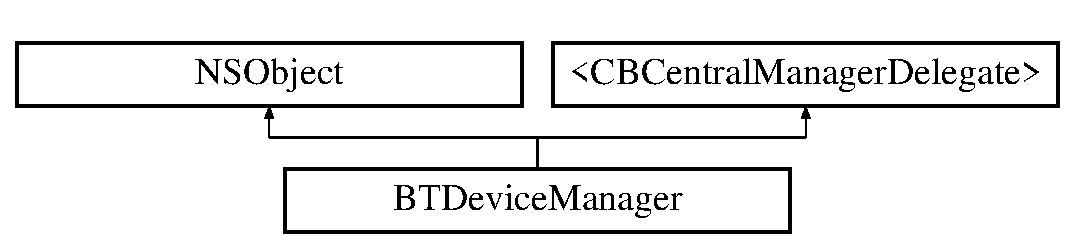
\includegraphics[height=2.000000cm]{interface_b_t_device_manager}
\end{center}
\end{figure}
\subsection*{Instance Methods}
\begin{DoxyCompactItemize}
\item 
(void) -\/ \hyperlink{interface_b_t_device_manager_a8ccfdb80e7396a787703df2e2145783b}{start\-Scan\-For\-Type\-:}
\item 
(N\-S\-Integer) -\/ \hyperlink{interface_b_t_device_manager_af88f5d1516142ed353cdcac2268dadfb}{discovered\-Devices\-For\-Type\-:}
\item 
(void) -\/ \hyperlink{interface_b_t_device_manager_a77d4c5c16c2e82bed7e5f2f65bcd2dfb}{stop\-Scan}
\item 
(void) -\/ \hyperlink{interface_b_t_device_manager_ae310a606d4e735e7813319e366f67aa2}{disconnect\-Selected\-Monitors}
\item 
(void) -\/ \hyperlink{interface_b_t_device_manager_afda16d6654df9d6eddde47c5a3ae38ec}{connect\-Selected\-Monitors}
\item 
(void) -\/ \hyperlink{interface_b_t_device_manager_aee2928325606cb3f338a5ecb8ef35560}{disconnect\-All\-Devices}
\item 
(void) -\/ \hyperlink{interface_b_t_device_manager_af3f435a6fec885eca732034a12239504}{select\-Device\-Type\-:at\-Index\-:}
\item 
(void) -\/ \hyperlink{interface_b_t_device_manager_a916adc15288fd7428a30954a57f0af0a}{deselect\-Device\-Type\-:}
\item 
(id$<$ \hyperlink{protocol_device_common_info_interface-p}{Device\-Common\-Info\-Interface} $>$) -\/ \hyperlink{interface_b_t_device_manager_a84c51142e50c343ffa90c5bf9afee48b}{device\-At\-Index\-:for\-Type\-:}
\item 
(id$<$ \hyperlink{protocol_device_common_info_interface-p}{Device\-Common\-Info\-Interface} $>$) -\/ \hyperlink{interface_b_t_device_manager_af11257d463445c307cd38c9e284c6826}{monitor\-Matching\-C\-B\-Peripheral\-:}
\item 
(id$<$ \hyperlink{protocol_heart_monitor_protocol-p}{Heart\-Monitor\-Protocol}, \\*
\hyperlink{protocol_device_common_info_interface-p}{Device\-Common\-Info\-Interface} $>$) -\/ \hyperlink{interface_b_t_device_manager_a1c4ad74783cb71a008c926f2e5ec3835}{selected\-Heart\-Monitor}
\item 
(void) -\/ \hyperlink{interface_b_t_device_manager_a005786995ec17c9a94e85a882bfd4896}{set\-Selected\-Heart\-Monitor\-:}
\item 
(id$<$ \hyperlink{protocol_activity_monitor_protocol-p}{Activity\-Monitor\-Protocol}, \\*
\hyperlink{protocol_device_common_info_interface-p}{Device\-Common\-Info\-Interface} $>$) -\/ \hyperlink{interface_b_t_device_manager_aaca0fdc9335bbc7465e91ad0f5c4dbb2}{selected\-Activity\-Monitor}
\item 
(void) -\/ \hyperlink{interface_b_t_device_manager_a6d8e2982b9a3ad004563736f89d98cb1}{set\-Selected\-Activity\-Monitor\-:}
\end{DoxyCompactItemize}
\subsection*{Class Methods}
\begin{DoxyCompactItemize}
\item 
(id) + \hyperlink{interface_b_t_device_manager_a38ff364ec62dc4ab4aea65f2aebed98c}{shared\-Manager}
\end{DoxyCompactItemize}
\subsection*{Properties}
\begin{DoxyCompactItemize}
\item 
id$<$ \hyperlink{protocol_heart_monitor_protocol-p}{Heart\-Monitor\-Protocol}, \\*
\hyperlink{protocol_device_common_info_interface-p}{Device\-Common\-Info\-Interface} $>$ \hyperlink{interface_b_t_device_manager_ab303b2617a6391db56c3b61f217f9b6b}{\-\_\-selected\-Heart\-Monitor}
\item 
id$<$ \hyperlink{protocol_activity_monitor_protocol-p}{Activity\-Monitor\-Protocol}, \\*
\hyperlink{protocol_device_common_info_interface-p}{Device\-Common\-Info\-Interface} $>$ \hyperlink{interface_b_t_device_manager_a53a05cc87797350638a2b82c337eb854}{\-\_\-selected\-Activity\-Monitor}
\item 
N\-S\-Array $\ast$ \hyperlink{interface_b_t_device_manager_a76ffd5887aa2d8c8ea20df2384851d41}{heart\-Devices}
\item 
N\-S\-Array $\ast$ \hyperlink{interface_b_t_device_manager_a8f6f577bb25b7dcd8b3857d6497bff4e}{activity\-Devices}
\item 
N\-S\-Integer \hyperlink{interface_b_t_device_manager_a98add70110c91e4266481e312d96afbf}{selected\-Index\-For\-Heart\-Monitor}
\item 
N\-S\-Integer \hyperlink{interface_b_t_device_manager_a8e47d59f0a40f8d96f4fea826be853d1}{selected\-Index\-For\-Activity\-Monitor}
\item 
B\-O\-O\-L \hyperlink{interface_b_t_device_manager_a15cc71749368c5de76624c5c4e4f7b3c}{is\-In\-Discovery\-Mode}
\item 
C\-B\-Central\-Manager $\ast$ \hyperlink{interface_b_t_device_manager_a61d03c41c000f28ce50e88bd9b8f6be9}{manager}
\item 
N\-S\-Integer \hyperlink{interface_b_t_device_manager_a610db66209e9d142e5451ceedc3c6a36}{search\-Type}
\item 
B\-O\-O\-L \hyperlink{interface_b_t_device_manager_a0864f241d9fc14f03e5f8e2b4dd0667a}{is\-Active}
\item 
N\-S\-Timer $\ast$ \hyperlink{interface_b_t_device_manager_aad4f780b6477ad7d37f6e85f3f40f1c0}{wait\-For\-Devices}
\item 
N\-S\-Run\-Loop $\ast$ \hyperlink{interface_b_t_device_manager_a2f3ce5cb472e8f042d4b427518d0ffea}{run\-Loop}
\item 
id \hyperlink{interface_b_t_device_manager_a53dc4023fb9a5873cd8f7a82489d25c0}{delegate}
\item 
N\-S\-Integer \hyperlink{interface_b_t_device_manager_ac70dac2c693cf191a05a606d7cea9763}{discovery\-Count}
\end{DoxyCompactItemize}


\subsection{Detailed Description}
This manager handles the overall connection and discovery of the bluetooth devices. It performs scanning, connectivity and management of the devices for the selection view controllers. This class is a singleton object because multiple instances cause problems with false posivitives for device connection and lost information based on O\-S level caching. W\-A\-R\-N\-I\-N\-G\-: Care must be take in assigning the delegate for this object. It is possible to produce side affects to other objects that are using this manager if care is not taken when updating this instance variable since the delegate can only reference one controlling object. 

\subsection{Method Documentation}
\hypertarget{interface_b_t_device_manager_afda16d6654df9d6eddde47c5a3ae38ec}{\index{B\-T\-Device\-Manager@{B\-T\-Device\-Manager}!connect\-Selected\-Monitors@{connect\-Selected\-Monitors}}
\index{connect\-Selected\-Monitors@{connect\-Selected\-Monitors}!BTDeviceManager@{B\-T\-Device\-Manager}}
\subsubsection[{connect\-Selected\-Monitors}]{\setlength{\rightskip}{0pt plus 5cm}-\/ (void) connect\-Selected\-Monitors 
\begin{DoxyParamCaption}
{}
\end{DoxyParamCaption}
}}\label{interface_b_t_device_manager_afda16d6654df9d6eddde47c5a3ae38ec}
This method connects the monitoring devices that have been selected from the various other views. It is used for the device poller to initiate the polling \hypertarget{interface_b_t_device_manager_a916adc15288fd7428a30954a57f0af0a}{\index{B\-T\-Device\-Manager@{B\-T\-Device\-Manager}!deselect\-Device\-Type\-:@{deselect\-Device\-Type\-:}}
\index{deselect\-Device\-Type\-:@{deselect\-Device\-Type\-:}!BTDeviceManager@{B\-T\-Device\-Manager}}
\subsubsection[{deselect\-Device\-Type\-:}]{\setlength{\rightskip}{0pt plus 5cm}-\/ (void) deselect\-Device\-Type\-: 
\begin{DoxyParamCaption}
\item[{(N\-S\-Integer)}]{type}
\end{DoxyParamCaption}
}}\label{interface_b_t_device_manager_a916adc15288fd7428a30954a57f0af0a}
This method is to be used by the tableviews so that individual devices can be deselected and the appropriate variables updated to reflect it.


\begin{DoxyParams}{Parameters}
{\em type} & The device type to deselect. See \hyperlink{_device_types_8h_source}{Device\-Types.\-h} for details. \\
\hline
\end{DoxyParams}
\hypertarget{interface_b_t_device_manager_a84c51142e50c343ffa90c5bf9afee48b}{\index{B\-T\-Device\-Manager@{B\-T\-Device\-Manager}!device\-At\-Index\-:for\-Type\-:@{device\-At\-Index\-:for\-Type\-:}}
\index{device\-At\-Index\-:for\-Type\-:@{device\-At\-Index\-:for\-Type\-:}!BTDeviceManager@{B\-T\-Device\-Manager}}
\subsubsection[{device\-At\-Index\-:for\-Type\-:}]{\setlength{\rightskip}{0pt plus 5cm}-\/ (id$<$ {\bf Device\-Common\-Info\-Interface} $>$) device\-At\-Index\-: 
\begin{DoxyParamCaption}
\item[{(N\-S\-Integer)}]{index}
\item[{forType:(N\-S\-Integer)}]{type}
\end{DoxyParamCaption}
}}\label{interface_b_t_device_manager_a84c51142e50c343ffa90c5bf9afee48b}
This method is used by the tableview to get the devices that they need to query for their views.


\begin{DoxyParams}{Parameters}
{\em index} & The index within the device types that are the same.\\
\hline
{\em type} & The device type that the search is restricted to performing.\\
\hline
\end{DoxyParams}
\begin{DoxyReturn}{Returns}
The device that is selected. The \hyperlink{protocol_device_common_info_interface-p}{Device\-Common\-Info\-Interface} is the restrictor and all devices must conform to this protocol, otherwise the result is nil. 
\end{DoxyReturn}
\hypertarget{interface_b_t_device_manager_aee2928325606cb3f338a5ecb8ef35560}{\index{B\-T\-Device\-Manager@{B\-T\-Device\-Manager}!disconnect\-All\-Devices@{disconnect\-All\-Devices}}
\index{disconnect\-All\-Devices@{disconnect\-All\-Devices}!BTDeviceManager@{B\-T\-Device\-Manager}}
\subsubsection[{disconnect\-All\-Devices}]{\setlength{\rightskip}{0pt plus 5cm}-\/ (void) disconnect\-All\-Devices 
\begin{DoxyParamCaption}
{}
\end{DoxyParamCaption}
}}\label{interface_b_t_device_manager_aee2928325606cb3f338a5ecb8ef35560}
This method is used to go through disconnecting every device after discovery. It is used when the viewcontrollers are being dismissed and the scanning is stopped. In order to discover all the characteristics needed for operation in other parts of the application, things like battery service, heart rate measurements etc must be discovered and that can only happen when the devices are connected. \hypertarget{interface_b_t_device_manager_ae310a606d4e735e7813319e366f67aa2}{\index{B\-T\-Device\-Manager@{B\-T\-Device\-Manager}!disconnect\-Selected\-Monitors@{disconnect\-Selected\-Monitors}}
\index{disconnect\-Selected\-Monitors@{disconnect\-Selected\-Monitors}!BTDeviceManager@{B\-T\-Device\-Manager}}
\subsubsection[{disconnect\-Selected\-Monitors}]{\setlength{\rightskip}{0pt plus 5cm}-\/ (void) disconnect\-Selected\-Monitors 
\begin{DoxyParamCaption}
{}
\end{DoxyParamCaption}
}}\label{interface_b_t_device_manager_ae310a606d4e735e7813319e366f67aa2}
This method is for disconnecting the devices that are used for monitoring. Both this method and the connect Monitors are meant to keep the battery lasting longer by not keeping connectivity when not in use. \hypertarget{interface_b_t_device_manager_af88f5d1516142ed353cdcac2268dadfb}{\index{B\-T\-Device\-Manager@{B\-T\-Device\-Manager}!discovered\-Devices\-For\-Type\-:@{discovered\-Devices\-For\-Type\-:}}
\index{discovered\-Devices\-For\-Type\-:@{discovered\-Devices\-For\-Type\-:}!BTDeviceManager@{B\-T\-Device\-Manager}}
\subsubsection[{discovered\-Devices\-For\-Type\-:}]{\setlength{\rightskip}{0pt plus 5cm}-\/ (N\-S\-Integer) discovered\-Devices\-For\-Type\-: 
\begin{DoxyParamCaption}
\item[{(N\-S\-Integer)}]{type}
\end{DoxyParamCaption}
}}\label{interface_b_t_device_manager_af88f5d1516142ed353cdcac2268dadfb}
This function gives the current count of the number of devices found in the discovery process based on the type of device it is looking to find. At this time there is H\-E\-A\-R\-T\-\_\-\-M\-O\-N\-I\-T\-O\-R and A\-C\-T\-I\-V\-I\-T\-Y\-\_\-\-M\-O\-N\-I\-T\-O\-R types. See \hyperlink{_device_types_8h_source}{Device\-Types.\-h} for more details.


\begin{DoxyParams}{Parameters}
{\em type} & The integer that designates whether a heart monitor or an activity monitor will be the attempt to discover.\\
\hline
\end{DoxyParams}
\begin{DoxyReturn}{Returns}
The number of devices found. 
\end{DoxyReturn}
\hypertarget{interface_b_t_device_manager_af11257d463445c307cd38c9e284c6826}{\index{B\-T\-Device\-Manager@{B\-T\-Device\-Manager}!monitor\-Matching\-C\-B\-Peripheral\-:@{monitor\-Matching\-C\-B\-Peripheral\-:}}
\index{monitor\-Matching\-C\-B\-Peripheral\-:@{monitor\-Matching\-C\-B\-Peripheral\-:}!BTDeviceManager@{B\-T\-Device\-Manager}}
\subsubsection[{monitor\-Matching\-C\-B\-Peripheral\-:}]{\setlength{\rightskip}{0pt plus 5cm}-\/ (id$<$ {\bf Device\-Common\-Info\-Interface} $>$) monitor\-Matching\-C\-B\-Peripheral\-: 
\begin{DoxyParamCaption}
\item[{(C\-B\-Peripheral$\ast$)}]{device}
\end{DoxyParamCaption}
}}\label{interface_b_t_device_manager_af11257d463445c307cd38c9e284c6826}
This is a method that is to be used privately in this class. It's purpose is to parse the list of devices that this manager knows about and return a device object that matches the C\-B\-Peripheral identifier. Since the identifier is a name it is possible to have two duplicate names. This is a change to C\-B\-Peripheral where the name takes precendence over the U\-U\-I\-D of the device if it is known.


\begin{DoxyParams}{Parameters}
{\em device} & The C\-B\-Peripheral that is to be used for the search criteria.\\
\hline
\end{DoxyParams}
\begin{DoxyReturn}{Returns}
A device object that conforms to the Common\-Device\-Info\-Interface. Additional introspection will be needed if you wish to see if the device conforms to one of the other protocols. 
\end{DoxyReturn}
\hypertarget{interface_b_t_device_manager_af3f435a6fec885eca732034a12239504}{\index{B\-T\-Device\-Manager@{B\-T\-Device\-Manager}!select\-Device\-Type\-:at\-Index\-:@{select\-Device\-Type\-:at\-Index\-:}}
\index{select\-Device\-Type\-:at\-Index\-:@{select\-Device\-Type\-:at\-Index\-:}!BTDeviceManager@{B\-T\-Device\-Manager}}
\subsubsection[{select\-Device\-Type\-:at\-Index\-:}]{\setlength{\rightskip}{0pt plus 5cm}-\/ (void) select\-Device\-Type\-: 
\begin{DoxyParamCaption}
\item[{(N\-S\-Integer)}]{type}
\item[{atIndex:(N\-S\-Integer)}]{index}
\end{DoxyParamCaption}
}}\label{interface_b_t_device_manager_af3f435a6fec885eca732034a12239504}
This method is to be used by the tableviews so that individual devices can be selected and the appropriate variables updated to reflect it.


\begin{DoxyParams}{Parameters}
{\em type} & The device type to select. See \hyperlink{_device_types_8h_source}{Device\-Types.\-h} for details.\\
\hline
{\em index} & The index of the array of devices within a particular type. \\
\hline
\end{DoxyParams}
\hypertarget{interface_b_t_device_manager_aaca0fdc9335bbc7465e91ad0f5c4dbb2}{\index{B\-T\-Device\-Manager@{B\-T\-Device\-Manager}!selected\-Activity\-Monitor@{selected\-Activity\-Monitor}}
\index{selected\-Activity\-Monitor@{selected\-Activity\-Monitor}!BTDeviceManager@{B\-T\-Device\-Manager}}
\subsubsection[{selected\-Activity\-Monitor}]{\setlength{\rightskip}{0pt plus 5cm}-\/ (id$<$ {\bf Activity\-Monitor\-Protocol}, {\bf Device\-Common\-Info\-Interface} $>$) selected\-Activity\-Monitor 
\begin{DoxyParamCaption}
{}
\end{DoxyParamCaption}
}}\label{interface_b_t_device_manager_aaca0fdc9335bbc7465e91ad0f5c4dbb2}
This getter returns the current selected\-Activity\-Monitor. The reference conforms to the \hyperlink{protocol_activity_monitor_protocol-p}{Activity\-Monitor\-Protocol} and the \hyperlink{protocol_device_common_info_interface-p}{Device\-Common\-Info\-Interface} protocol.

\begin{DoxyReturn}{Returns}
the object reference for the activity monitor. A check for nil is necessary because it is possible to deselect the activity monitor. 
\end{DoxyReturn}
\hypertarget{interface_b_t_device_manager_a1c4ad74783cb71a008c926f2e5ec3835}{\index{B\-T\-Device\-Manager@{B\-T\-Device\-Manager}!selected\-Heart\-Monitor@{selected\-Heart\-Monitor}}
\index{selected\-Heart\-Monitor@{selected\-Heart\-Monitor}!BTDeviceManager@{B\-T\-Device\-Manager}}
\subsubsection[{selected\-Heart\-Monitor}]{\setlength{\rightskip}{0pt plus 5cm}-\/ (id$<$ {\bf Heart\-Monitor\-Protocol}, {\bf Device\-Common\-Info\-Interface} $>$) selected\-Heart\-Monitor 
\begin{DoxyParamCaption}
{}
\end{DoxyParamCaption}
}}\label{interface_b_t_device_manager_a1c4ad74783cb71a008c926f2e5ec3835}
This getter returns the current selected\-Heart\-Monitor. The reference conforms to the \hyperlink{protocol_heart_monitor_protocol-p}{Heart\-Monitor\-Protocol} and the \hyperlink{protocol_device_common_info_interface-p}{Device\-Common\-Info\-Interface} protocol.

\begin{DoxyReturn}{Returns}
the object reference for the heart monitor. A check for nil is necessary because it is possible to deselect the heart monitor. 
\end{DoxyReturn}
\hypertarget{interface_b_t_device_manager_a6d8e2982b9a3ad004563736f89d98cb1}{\index{B\-T\-Device\-Manager@{B\-T\-Device\-Manager}!set\-Selected\-Activity\-Monitor\-:@{set\-Selected\-Activity\-Monitor\-:}}
\index{set\-Selected\-Activity\-Monitor\-:@{set\-Selected\-Activity\-Monitor\-:}!BTDeviceManager@{B\-T\-Device\-Manager}}
\subsubsection[{set\-Selected\-Activity\-Monitor\-:}]{\setlength{\rightskip}{0pt plus 5cm}-\/ (void) set\-Selected\-Activity\-Monitor\-: 
\begin{DoxyParamCaption}
\item[{(id$<${\bf Activity\-Monitor\-Protocol}, {\bf Device\-Common\-Info\-Interface}$>$)}]{selected\-Activity\-Monitor}
\end{DoxyParamCaption}
}}\label{interface_b_t_device_manager_a6d8e2982b9a3ad004563736f89d98cb1}
This setter updates the selected\-Activity\-Monitor as long as it conforms to the \hyperlink{protocol_activity_monitor_protocol-p}{Activity\-Monitor\-Protocol} and the \hyperlink{protocol_device_common_info_interface-p}{Device\-Common\-Info\-Interface}. It also notifies that delegate that the value has changed.


\begin{DoxyParams}{Parameters}
{\em selected\-Activity\-Monitor} & The activity monitor that has been selected by the view controller. \\
\hline
\end{DoxyParams}
\hypertarget{interface_b_t_device_manager_a005786995ec17c9a94e85a882bfd4896}{\index{B\-T\-Device\-Manager@{B\-T\-Device\-Manager}!set\-Selected\-Heart\-Monitor\-:@{set\-Selected\-Heart\-Monitor\-:}}
\index{set\-Selected\-Heart\-Monitor\-:@{set\-Selected\-Heart\-Monitor\-:}!BTDeviceManager@{B\-T\-Device\-Manager}}
\subsubsection[{set\-Selected\-Heart\-Monitor\-:}]{\setlength{\rightskip}{0pt plus 5cm}-\/ (void) set\-Selected\-Heart\-Monitor\-: 
\begin{DoxyParamCaption}
\item[{(id$<${\bf Heart\-Monitor\-Protocol}, {\bf Device\-Common\-Info\-Interface}$>$)}]{selected\-Heart\-Monitor}
\end{DoxyParamCaption}
}}\label{interface_b_t_device_manager_a005786995ec17c9a94e85a882bfd4896}
This setter updates the selected\-Heart\-Monitor as long as it conforms to the \hyperlink{protocol_heart_monitor_protocol-p}{Heart\-Monitor\-Protocol} and the \hyperlink{protocol_device_common_info_interface-p}{Device\-Common\-Info\-Interface}. It also notifies that delegate that the value has changed.


\begin{DoxyParams}{Parameters}
{\em selected\-Heart\-Monitor} & The heart mo0nitor that has been selected by the view controller. \\
\hline
\end{DoxyParams}
\hypertarget{interface_b_t_device_manager_a38ff364ec62dc4ab4aea65f2aebed98c}{\index{B\-T\-Device\-Manager@{B\-T\-Device\-Manager}!shared\-Manager@{shared\-Manager}}
\index{shared\-Manager@{shared\-Manager}!BTDeviceManager@{B\-T\-Device\-Manager}}
\subsubsection[{shared\-Manager}]{\setlength{\rightskip}{0pt plus 5cm}+ (id) shared\-Manager 
\begin{DoxyParamCaption}
{}
\end{DoxyParamCaption}
}}\label{interface_b_t_device_manager_a38ff364ec62dc4ab4aea65f2aebed98c}
This is the preferred method of initialization. This object is treated as a singleton because nil objects and other conflicts will result from using more than one instance of a C\-B\-Central object, which is included in this object.

\begin{DoxyReturn}{Returns}
The shared instance of a \hyperlink{interface_b_t_device_manager}{B\-T\-Device\-Manager}. 
\end{DoxyReturn}
\hypertarget{interface_b_t_device_manager_a8ccfdb80e7396a787703df2e2145783b}{\index{B\-T\-Device\-Manager@{B\-T\-Device\-Manager}!start\-Scan\-For\-Type\-:@{start\-Scan\-For\-Type\-:}}
\index{start\-Scan\-For\-Type\-:@{start\-Scan\-For\-Type\-:}!BTDeviceManager@{B\-T\-Device\-Manager}}
\subsubsection[{start\-Scan\-For\-Type\-:}]{\setlength{\rightskip}{0pt plus 5cm}-\/ (void) start\-Scan\-For\-Type\-: 
\begin{DoxyParamCaption}
\item[{(N\-S\-Integer)}]{type}
\end{DoxyParamCaption}
}}\label{interface_b_t_device_manager_a8ccfdb80e7396a787703df2e2145783b}
This method starts the scanning process for a particular type of device. See \hyperlink{_device_types_8h_source}{Device\-Types.\-h} for values relating to the kind of device to scan.


\begin{DoxyParams}{Parameters}
{\em type} & The integer value representing the kind of services to scan and discover. \\
\hline
\end{DoxyParams}
\hypertarget{interface_b_t_device_manager_a77d4c5c16c2e82bed7e5f2f65bcd2dfb}{\index{B\-T\-Device\-Manager@{B\-T\-Device\-Manager}!stop\-Scan@{stop\-Scan}}
\index{stop\-Scan@{stop\-Scan}!BTDeviceManager@{B\-T\-Device\-Manager}}
\subsubsection[{stop\-Scan}]{\setlength{\rightskip}{0pt plus 5cm}-\/ (void) stop\-Scan 
\begin{DoxyParamCaption}
{}
\end{DoxyParamCaption}
}}\label{interface_b_t_device_manager_a77d4c5c16c2e82bed7e5f2f65bcd2dfb}
This function allows remote shutdown of discovery process to conserve the battery. Its purpose is to allow the dismissal of selection viewcontrollers to shut the discovery because the devicemanager class is shared throughout the application. 

\subsection{Property Documentation}
\hypertarget{interface_b_t_device_manager_a53a05cc87797350638a2b82c337eb854}{\index{B\-T\-Device\-Manager@{B\-T\-Device\-Manager}!\-\_\-selected\-Activity\-Monitor@{\-\_\-selected\-Activity\-Monitor}}
\index{\-\_\-selected\-Activity\-Monitor@{\-\_\-selected\-Activity\-Monitor}!BTDeviceManager@{B\-T\-Device\-Manager}}
\subsubsection[{\-\_\-selected\-Activity\-Monitor}]{\setlength{\rightskip}{0pt plus 5cm}-\/ (id$<${\bf Activity\-Monitor\-Protocol}, {\bf Device\-Common\-Info\-Interface}$>$) \-\_\-selected\-Activity\-Monitor\hspace{0.3cm}{\ttfamily [read]}, {\ttfamily [write]}, {\ttfamily [atomic]}}}\label{interface_b_t_device_manager_a53a05cc87797350638a2b82c337eb854}
The activity monitor that is currently selected. The value may be nil when nothing is selected and is part of the design. This variable should only be accessed using selected\-Activity\-Monitor and set\-Selected\-Activity\-Monitor because the delegate is notified of any changes to this value. \hypertarget{interface_b_t_device_manager_ab303b2617a6391db56c3b61f217f9b6b}{\index{B\-T\-Device\-Manager@{B\-T\-Device\-Manager}!\-\_\-selected\-Heart\-Monitor@{\-\_\-selected\-Heart\-Monitor}}
\index{\-\_\-selected\-Heart\-Monitor@{\-\_\-selected\-Heart\-Monitor}!BTDeviceManager@{B\-T\-Device\-Manager}}
\subsubsection[{\-\_\-selected\-Heart\-Monitor}]{\setlength{\rightskip}{0pt plus 5cm}-\/ (id$<${\bf Heart\-Monitor\-Protocol}, {\bf Device\-Common\-Info\-Interface}$>$) \-\_\-selected\-Heart\-Monitor\hspace{0.3cm}{\ttfamily [read]}, {\ttfamily [write]}, {\ttfamily [atomic]}}}\label{interface_b_t_device_manager_ab303b2617a6391db56c3b61f217f9b6b}
The heart monitor that is currently selected. The value may be nil when nothing is selected and is part of the design. This variable should only be accessed using selected\-Heart\-Monitor and set\-Selected\-Heart\-Monitor because the delegate is notified of any changes to this value. \hypertarget{interface_b_t_device_manager_a8f6f577bb25b7dcd8b3857d6497bff4e}{\index{B\-T\-Device\-Manager@{B\-T\-Device\-Manager}!activity\-Devices@{activity\-Devices}}
\index{activity\-Devices@{activity\-Devices}!BTDeviceManager@{B\-T\-Device\-Manager}}
\subsubsection[{activity\-Devices}]{\setlength{\rightskip}{0pt plus 5cm}-\/ (N\-S\-Array$\ast$) activity\-Devices\hspace{0.3cm}{\ttfamily [read]}, {\ttfamily [write]}, {\ttfamily [atomic]}}}\label{interface_b_t_device_manager_a8f6f577bb25b7dcd8b3857d6497bff4e}
The array containing any devices that conform to the \hyperlink{protocol_activity_monitor_protocol-p}{Activity\-Monitor\-Protocol}. It is used by the activity monitor selection view controller for listing possible devices to use. \hypertarget{interface_b_t_device_manager_a53dc4023fb9a5873cd8f7a82489d25c0}{\index{B\-T\-Device\-Manager@{B\-T\-Device\-Manager}!delegate@{delegate}}
\index{delegate@{delegate}!BTDeviceManager@{B\-T\-Device\-Manager}}
\subsubsection[{delegate}]{\setlength{\rightskip}{0pt plus 5cm}-\/ (id) delegate\hspace{0.3cm}{\ttfamily [read]}, {\ttfamily [write]}, {\ttfamily [nonatomic]}, {\ttfamily [weak]}}}\label{interface_b_t_device_manager_a53dc4023fb9a5873cd8f7a82489d25c0}
The delegate is the object that receives a call back whenever the selected heart monitor or activity monitor has changed. \hypertarget{interface_b_t_device_manager_ac70dac2c693cf191a05a606d7cea9763}{\index{B\-T\-Device\-Manager@{B\-T\-Device\-Manager}!discovery\-Count@{discovery\-Count}}
\index{discovery\-Count@{discovery\-Count}!BTDeviceManager@{B\-T\-Device\-Manager}}
\subsubsection[{discovery\-Count}]{\setlength{\rightskip}{0pt plus 5cm}-\/ (N\-S\-Integer) discovery\-Count\hspace{0.3cm}{\ttfamily [read]}, {\ttfamily [write]}, {\ttfamily [atomic]}}}\label{interface_b_t_device_manager_ac70dac2c693cf191a05a606d7cea9763}
The counter that is used for requesting a new discovery of the device. The setting is 5 seconds, and then a rediscovery of the device begins. \hypertarget{interface_b_t_device_manager_a76ffd5887aa2d8c8ea20df2384851d41}{\index{B\-T\-Device\-Manager@{B\-T\-Device\-Manager}!heart\-Devices@{heart\-Devices}}
\index{heart\-Devices@{heart\-Devices}!BTDeviceManager@{B\-T\-Device\-Manager}}
\subsubsection[{heart\-Devices}]{\setlength{\rightskip}{0pt plus 5cm}-\/ (N\-S\-Array$\ast$) heart\-Devices\hspace{0.3cm}{\ttfamily [read]}, {\ttfamily [write]}, {\ttfamily [atomic]}}}\label{interface_b_t_device_manager_a76ffd5887aa2d8c8ea20df2384851d41}
The array containing any devices that conform to the \hyperlink{protocol_heart_monitor_protocol-p}{Heart\-Monitor\-Protocol}. It is used by the heart monitor selection view controller for listing possible devices to use. \hypertarget{interface_b_t_device_manager_a0864f241d9fc14f03e5f8e2b4dd0667a}{\index{B\-T\-Device\-Manager@{B\-T\-Device\-Manager}!is\-Active@{is\-Active}}
\index{is\-Active@{is\-Active}!BTDeviceManager@{B\-T\-Device\-Manager}}
\subsubsection[{is\-Active}]{\setlength{\rightskip}{0pt plus 5cm}-\/ (B\-O\-O\-L) is\-Active\hspace{0.3cm}{\ttfamily [read]}, {\ttfamily [write]}, {\ttfamily [atomic]}}}\label{interface_b_t_device_manager_a0864f241d9fc14f03e5f8e2b4dd0667a}
This flag is to see if bluetooth use is allowed. The manager will not be able to perform any operations if the bluetooth service is off or not allowed by the user. \hypertarget{interface_b_t_device_manager_a15cc71749368c5de76624c5c4e4f7b3c}{\index{B\-T\-Device\-Manager@{B\-T\-Device\-Manager}!is\-In\-Discovery\-Mode@{is\-In\-Discovery\-Mode}}
\index{is\-In\-Discovery\-Mode@{is\-In\-Discovery\-Mode}!BTDeviceManager@{B\-T\-Device\-Manager}}
\subsubsection[{is\-In\-Discovery\-Mode}]{\setlength{\rightskip}{0pt plus 5cm}-\/ (B\-O\-O\-L) is\-In\-Discovery\-Mode\hspace{0.3cm}{\ttfamily [read]}, {\ttfamily [write]}, {\ttfamily [atomic]}}}\label{interface_b_t_device_manager_a15cc71749368c5de76624c5c4e4f7b3c}
This flag indicates that the manager is in discovery mode and that addition scans must be performed to get the characteristics and services of the devices as they are discovered and connected. \hypertarget{interface_b_t_device_manager_a61d03c41c000f28ce50e88bd9b8f6be9}{\index{B\-T\-Device\-Manager@{B\-T\-Device\-Manager}!manager@{manager}}
\index{manager@{manager}!BTDeviceManager@{B\-T\-Device\-Manager}}
\subsubsection[{manager}]{\setlength{\rightskip}{0pt plus 5cm}-\/ (C\-B\-Central\-Manager$\ast$) manager\hspace{0.3cm}{\ttfamily [read]}, {\ttfamily [write]}, {\ttfamily [atomic]}, {\ttfamily [retain]}}}\label{interface_b_t_device_manager_a61d03c41c000f28ce50e88bd9b8f6be9}
The bluetooth connection manager that tracks the C\-B\-Peripherals. \hypertarget{interface_b_t_device_manager_a2f3ce5cb472e8f042d4b427518d0ffea}{\index{B\-T\-Device\-Manager@{B\-T\-Device\-Manager}!run\-Loop@{run\-Loop}}
\index{run\-Loop@{run\-Loop}!BTDeviceManager@{B\-T\-Device\-Manager}}
\subsubsection[{run\-Loop}]{\setlength{\rightskip}{0pt plus 5cm}-\/ (N\-S\-Run\-Loop$\ast$) run\-Loop\hspace{0.3cm}{\ttfamily [read]}, {\ttfamily [write]}, {\ttfamily [atomic]}}}\label{interface_b_t_device_manager_a2f3ce5cb472e8f042d4b427518d0ffea}
The runloop that is used to check for device discovery to see if all characteristics needed have been discovered. The reference is stated so it can be canceld outside the method that calls it. \hypertarget{interface_b_t_device_manager_a610db66209e9d142e5451ceedc3c6a36}{\index{B\-T\-Device\-Manager@{B\-T\-Device\-Manager}!search\-Type@{search\-Type}}
\index{search\-Type@{search\-Type}!BTDeviceManager@{B\-T\-Device\-Manager}}
\subsubsection[{search\-Type}]{\setlength{\rightskip}{0pt plus 5cm}-\/ (N\-S\-Integer) search\-Type\hspace{0.3cm}{\ttfamily [read]}, {\ttfamily [write]}, {\ttfamily [atomic]}}}\label{interface_b_t_device_manager_a610db66209e9d142e5451ceedc3c6a36}
This value indicates what services the manager should scan and connect. For details see \hyperlink{_device_types_8h_source}{Device\-Types.\-h} \hypertarget{interface_b_t_device_manager_a8e47d59f0a40f8d96f4fea826be853d1}{\index{B\-T\-Device\-Manager@{B\-T\-Device\-Manager}!selected\-Index\-For\-Activity\-Monitor@{selected\-Index\-For\-Activity\-Monitor}}
\index{selected\-Index\-For\-Activity\-Monitor@{selected\-Index\-For\-Activity\-Monitor}!BTDeviceManager@{B\-T\-Device\-Manager}}
\subsubsection[{selected\-Index\-For\-Activity\-Monitor}]{\setlength{\rightskip}{0pt plus 5cm}-\/ (N\-S\-Integer) selected\-Index\-For\-Activity\-Monitor\hspace{0.3cm}{\ttfamily [read]}, {\ttfamily [write]}, {\ttfamily [atomic]}}}\label{interface_b_t_device_manager_a8e47d59f0a40f8d96f4fea826be853d1}
The index of the activity monitor device that has been selected. It is used by the activity monitor select view controller to indicate which one is selected. If the value is -\/1, then no device has been selected. \hypertarget{interface_b_t_device_manager_a98add70110c91e4266481e312d96afbf}{\index{B\-T\-Device\-Manager@{B\-T\-Device\-Manager}!selected\-Index\-For\-Heart\-Monitor@{selected\-Index\-For\-Heart\-Monitor}}
\index{selected\-Index\-For\-Heart\-Monitor@{selected\-Index\-For\-Heart\-Monitor}!BTDeviceManager@{B\-T\-Device\-Manager}}
\subsubsection[{selected\-Index\-For\-Heart\-Monitor}]{\setlength{\rightskip}{0pt plus 5cm}-\/ (N\-S\-Integer) selected\-Index\-For\-Heart\-Monitor\hspace{0.3cm}{\ttfamily [read]}, {\ttfamily [write]}, {\ttfamily [atomic]}}}\label{interface_b_t_device_manager_a98add70110c91e4266481e312d96afbf}
The index of the heart monitor device that has been selected. It is used by the heart monitor select view controller to indicate which one is selected. If the value is -\/1, then no device has been selected. \hypertarget{interface_b_t_device_manager_aad4f780b6477ad7d37f6e85f3f40f1c0}{\index{B\-T\-Device\-Manager@{B\-T\-Device\-Manager}!wait\-For\-Devices@{wait\-For\-Devices}}
\index{wait\-For\-Devices@{wait\-For\-Devices}!BTDeviceManager@{B\-T\-Device\-Manager}}
\subsubsection[{wait\-For\-Devices}]{\setlength{\rightskip}{0pt plus 5cm}-\/ (N\-S\-Timer$\ast$) wait\-For\-Devices\hspace{0.3cm}{\ttfamily [read]}, {\ttfamily [write]}, {\ttfamily [atomic]}}}\label{interface_b_t_device_manager_aad4f780b6477ad7d37f6e85f3f40f1c0}
The timer that is used when the request to stop scanning has been done, but the device that is selected does not have full discovery done. 

The documentation for this class was generated from the following files\-:\begin{DoxyCompactItemize}
\item 
/\-Users/douglas/\-Documents/software/\-Senior Project/ios/\-Medical Cyborgs/\-Medical Cyborgs/B\-T\-Device\-Manager.\-h\item 
/\-Users/douglas/\-Documents/software/\-Senior Project/ios/\-Medical Cyborgs/\-Medical Cyborgs/B\-T\-Device\-Manager.\-m\end{DoxyCompactItemize}

\hypertarget{protocol_b_t_device_manager_delegate-p}{\section{$<$B\-T\-Device\-Manager\-Delegate$>$ Protocol Reference}
\label{protocol_b_t_device_manager_delegate-p}\index{$<$\-B\-T\-Device\-Manager\-Delegate$>$@{$<$\-B\-T\-Device\-Manager\-Delegate$>$}}
}


{\ttfamily \#import $<$B\-T\-Device\-Manager\-Delegate.\-h$>$}

Inheritance diagram for $<$B\-T\-Device\-Manager\-Delegate$>$\-:\begin{figure}[H]
\begin{center}
\leavevmode
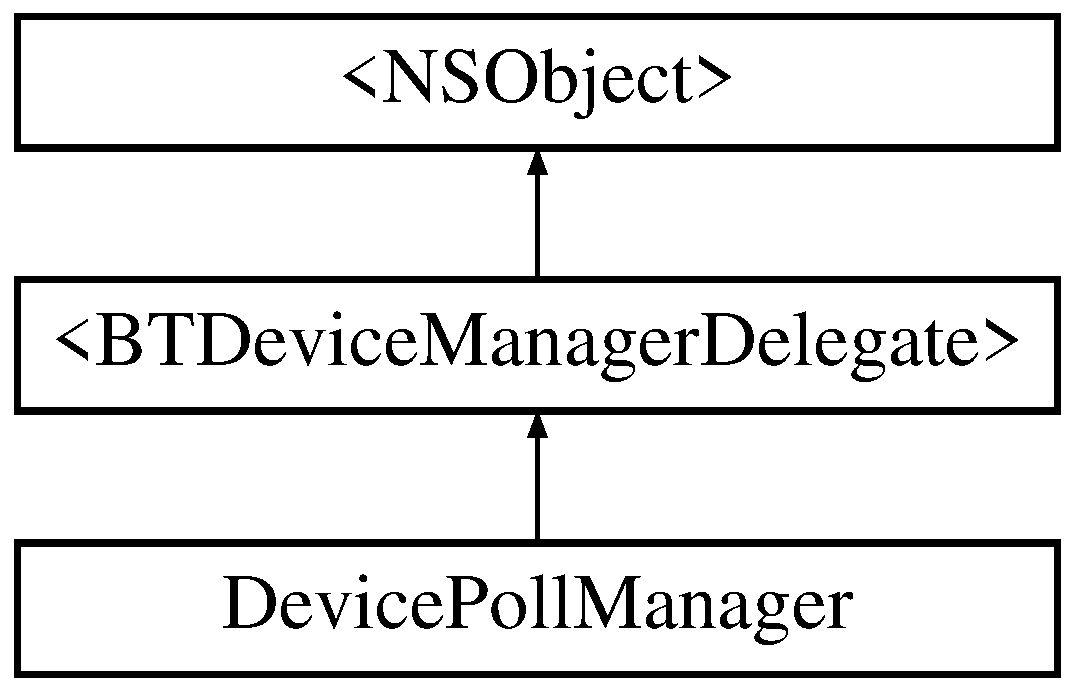
\includegraphics[height=3.000000cm]{protocol_b_t_device_manager_delegate-p}
\end{center}
\end{figure}
\subsection*{Instance Methods}
\begin{DoxyCompactItemize}
\item 
(void) -\/ \hyperlink{protocol_b_t_device_manager_delegate-p_afc2437f8a5b807ef0c173afb08af7fef}{device\-Manager\-Did\-Update\-Monitors}
\end{DoxyCompactItemize}


\subsection{Detailed Description}
The protocol is used for delegate of the \hyperlink{interface_b_t_device_manager}{B\-T\-Device\-Manager} for callback to notifiy the delegate that changes have been made to selected monitors. 

\subsection{Method Documentation}
\hypertarget{protocol_b_t_device_manager_delegate-p_afc2437f8a5b807ef0c173afb08af7fef}{\index{B\-T\-Device\-Manager\-Delegate-\/p@{B\-T\-Device\-Manager\-Delegate-\/p}!device\-Manager\-Did\-Update\-Monitors@{device\-Manager\-Did\-Update\-Monitors}}
\index{device\-Manager\-Did\-Update\-Monitors@{device\-Manager\-Did\-Update\-Monitors}!BTDeviceManagerDelegate-p@{B\-T\-Device\-Manager\-Delegate-\/p}}
\subsubsection[{device\-Manager\-Did\-Update\-Monitors}]{\setlength{\rightskip}{0pt plus 5cm}-\/ (void) device\-Manager\-Did\-Update\-Monitors 
\begin{DoxyParamCaption}
{}
\end{DoxyParamCaption}
\hspace{0.3cm}{\ttfamily [required]}}}\label{protocol_b_t_device_manager_delegate-p_afc2437f8a5b807ef0c173afb08af7fef}
This method is called by the \hyperlink{interface_b_t_device_manager}{B\-T\-Device\-Manager} after the selected\-Heart\-Monitor or the select\-Activity\-Monitor references have changed. 

The documentation for this protocol was generated from the following file\-:\begin{DoxyCompactItemize}
\item 
/\-Users/douglas/\-Documents/software/\-Senior Project/ios/\-Medical Cyborgs/\-Medical Cyborgs/B\-T\-Device\-Manager\-Delegate.\-h\end{DoxyCompactItemize}

\hypertarget{interface_d_b_manager}{\section{D\-B\-Manager Class Reference}
\label{interface_d_b_manager}\index{D\-B\-Manager@{D\-B\-Manager}}
}


{\ttfamily \#import $<$D\-B\-Manager.\-h$>$}

Inheritance diagram for D\-B\-Manager\-:\begin{figure}[H]
\begin{center}
\leavevmode
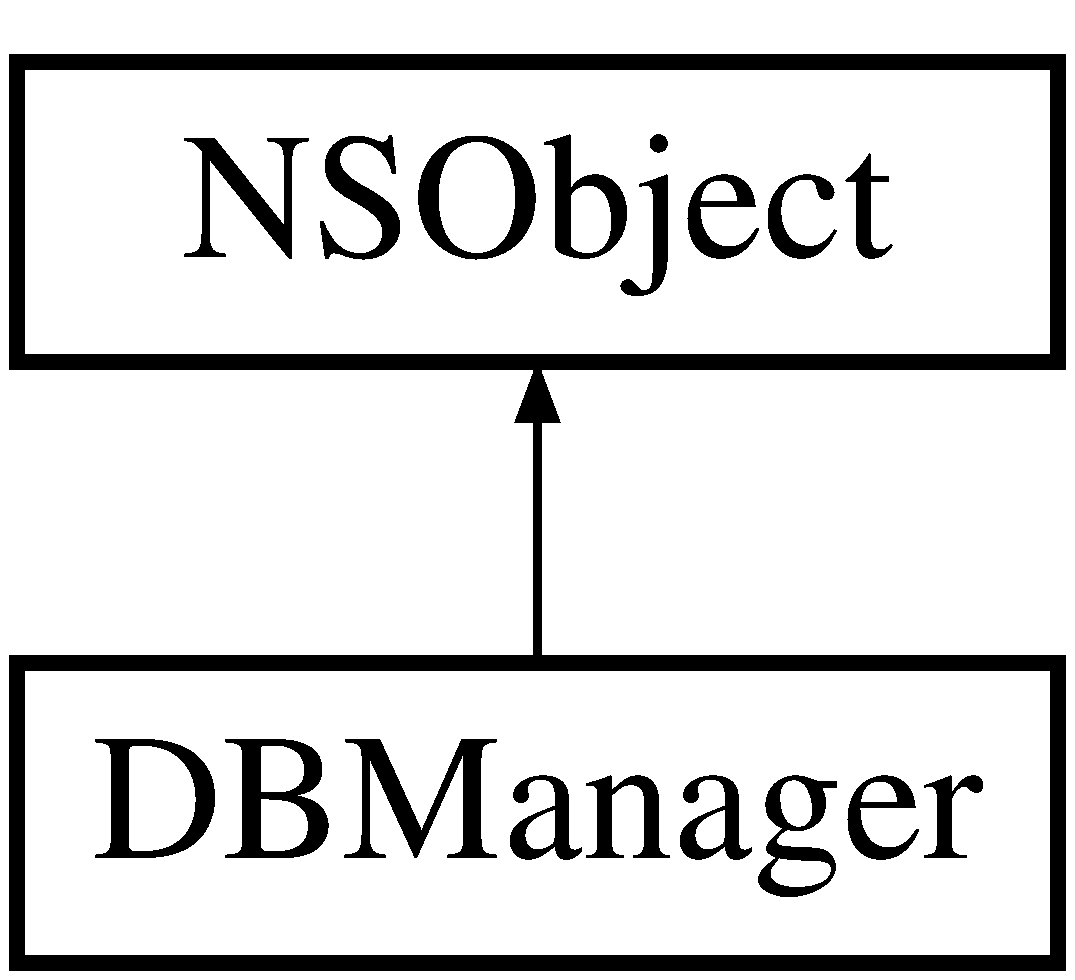
\includegraphics[height=2.000000cm]{interface_d_b_manager}
\end{center}
\end{figure}
\subsection*{Instance Methods}
\begin{DoxyCompactItemize}
\item 
(instancetype) -\/ \hyperlink{interface_d_b_manager_a0b390c8eab2577c30b2012e14ae821fe}{init}
\item 
(instancetype) -\/ \hyperlink{interface_d_b_manager_a24ba5578b7bcfff67ad5fcffb6c05f7b}{init\-Withpatient\-I\-D\-:}
\item 
(void) -\/ \hyperlink{interface_d_b_manager_a2e49fe020ebf348c2768a4c4a3dcff00}{copy\-Database\-Into\-Documents\-Directory}
\item 
(\hyperlink{interface_local_d_b_result}{Local\-D\-B\-Result} $\ast$) -\/ \hyperlink{interface_d_b_manager_ad6723b4f6b2191eddbcc4bb9bd361fcb}{retrieve\-Row}
\item 
(B\-O\-O\-L) -\/ \hyperlink{interface_d_b_manager_a3c424eba24e9894922714f6154a6dc44}{is\-Database\-Empty}
\item 
(void) -\/ \hyperlink{interface_d_b_manager_a0c354ea19fc86923ba33e5dc32798ca8}{insert\-Data\-Into\-D\-B}
\item 
(void) -\/ \hyperlink{interface_d_b_manager_a28d37edd37bc78b35579d276b8abfd9b}{delete\-Row\-At\-Time\-Stamp\-:}
\item 
(B\-O\-O\-L) -\/ \hyperlink{interface_d_b_manager_ab93660b0ab1caac6cd83b9edc349ddee}{open\-Local\-D\-B\-With\-S\-Q\-L\-Query\-Is\-Successful\-:}
\item 
(void) -\/ \hyperlink{interface_d_b_manager_a768157b5a58c4e400ee1326fe804d2b8}{close\-Local\-D\-B\-Connection}
\item 
(void) -\/ \hyperlink{interface_d_b_manager_aa804a3f4200ce732321d814cf86dbd2b}{purge\-Database}
\end{DoxyCompactItemize}
\subsection*{Class Methods}
\begin{DoxyCompactItemize}
\item 
(N\-S\-String $\ast$) + \hyperlink{interface_d_b_manager_a7c8d65202b11dbd5c926bc6a01c4259d}{time\-Stamp\-As\-String\-:}
\end{DoxyCompactItemize}
\subsection*{Properties}
\begin{DoxyCompactItemize}
\item 
\hypertarget{interface_d_b_manager_a2da5077535faad528421bada70121866}{N\-S\-String $\ast$ {\bfseries documents\-Directory}}\label{interface_d_b_manager_a2da5077535faad528421bada70121866}

\item 
\hypertarget{interface_d_b_manager_a725c101d5daf6506b59e0f7e06993982}{N\-S\-String $\ast$ {\bfseries database\-Filename}}\label{interface_d_b_manager_a725c101d5daf6506b59e0f7e06993982}

\item 
\hypertarget{interface_d_b_manager_a7206acae059164df418a2dbfaa7fbb13}{N\-S\-Integer {\bfseries patient\-I\-D}}\label{interface_d_b_manager_a7206acae059164df418a2dbfaa7fbb13}

\item 
\hypertarget{interface_d_b_manager_a921cb5034e1b4f79c6db59a1ce3fd579}{B\-O\-O\-L {\bfseries more\-Rows\-To\-Retrieve}}\label{interface_d_b_manager_a921cb5034e1b4f79c6db59a1ce3fd579}

\item 
\hypertarget{interface_d_b_manager_aa3315763d817eb3c10dac39ee530e2a8}{sqlite3 $\ast$ {\bfseries database}}\label{interface_d_b_manager_aa3315763d817eb3c10dac39ee530e2a8}

\item 
\hypertarget{interface_d_b_manager_a7299e28bee3f75281496adcebb46010b}{N\-S\-Integer {\bfseries row\-Count}}\label{interface_d_b_manager_a7299e28bee3f75281496adcebb46010b}

\item 
\hypertarget{interface_d_b_manager_a15a4e85cdc292d83ee3d8b28e43c43bc}{N\-S\-String $\ast$ {\bfseries database\-Path}}\label{interface_d_b_manager_a15a4e85cdc292d83ee3d8b28e43c43bc}

\item 
\hypertarget{interface_d_b_manager_ae714f21433f7593c722b727d2ae9c66a}{sqlite3\-\_\-stmt $\ast$ {\bfseries sql\-Statement}}\label{interface_d_b_manager_ae714f21433f7593c722b727d2ae9c66a}

\item 
\hypertarget{interface_d_b_manager_ac89481f8c2c45def2b8edb2ba749df68}{N\-S\-Integer {\bfseries hrmeasurement}}\label{interface_d_b_manager_ac89481f8c2c45def2b8edb2ba749df68}

\item 
\hypertarget{interface_d_b_manager_a12dcee066d2cecde8507a6529df92521}{float {\bfseries latitude}}\label{interface_d_b_manager_a12dcee066d2cecde8507a6529df92521}

\item 
\hypertarget{interface_d_b_manager_aa881cd8f0940350240e3ae9a326e5563}{float {\bfseries longitude}}\label{interface_d_b_manager_aa881cd8f0940350240e3ae9a326e5563}

\item 
\hypertarget{interface_d_b_manager_aff07ccf2439a2df78a5375303d5272a7}{int {\bfseries activity\-Level}}\label{interface_d_b_manager_aff07ccf2439a2df78a5375303d5272a7}

\item 
\hypertarget{interface_d_b_manager_a0d952846514339beeb1ff00a89fd650e}{N\-S\-Integer {\bfseries age}}\label{interface_d_b_manager_a0d952846514339beeb1ff00a89fd650e}

\item 
\hypertarget{interface_d_b_manager_a62443c98d9fade6ab9906836bf146b72}{N\-S\-Date $\ast$ {\bfseries timestamp}}\label{interface_d_b_manager_a62443c98d9fade6ab9906836bf146b72}

\end{DoxyCompactItemize}


\subsection{Detailed Description}
This class handles the local S\-Q\-L\-I\-T\-E3 database. All functions needed to use this database are enclosed in the class. 

\subsection{Method Documentation}
\hypertarget{interface_d_b_manager_a768157b5a58c4e400ee1326fe804d2b8}{\index{D\-B\-Manager@{D\-B\-Manager}!close\-Local\-D\-B\-Connection@{close\-Local\-D\-B\-Connection}}
\index{close\-Local\-D\-B\-Connection@{close\-Local\-D\-B\-Connection}!DBManager@{D\-B\-Manager}}
\subsubsection[{close\-Local\-D\-B\-Connection}]{\setlength{\rightskip}{0pt plus 5cm}-\/ (void) close\-Local\-D\-B\-Connection 
\begin{DoxyParamCaption}
{}
\end{DoxyParamCaption}
}}\label{interface_d_b_manager_a768157b5a58c4e400ee1326fe804d2b8}
This method is meant to be a private method. It is meant to finalize the database and close the database. All results from the query will be lost as memory is freed during finalization. \hypertarget{interface_d_b_manager_a2e49fe020ebf348c2768a4c4a3dcff00}{\index{D\-B\-Manager@{D\-B\-Manager}!copy\-Database\-Into\-Documents\-Directory@{copy\-Database\-Into\-Documents\-Directory}}
\index{copy\-Database\-Into\-Documents\-Directory@{copy\-Database\-Into\-Documents\-Directory}!DBManager@{D\-B\-Manager}}
\subsubsection[{copy\-Database\-Into\-Documents\-Directory}]{\setlength{\rightskip}{0pt plus 5cm}-\/ (void) copy\-Database\-Into\-Documents\-Directory 
\begin{DoxyParamCaption}
{}
\end{DoxyParamCaption}
}}\label{interface_d_b_manager_a2e49fe020ebf348c2768a4c4a3dcff00}
This method is used for first time use of the application. It copies the master database template to the applications Documents directory for use with the application. W\-A\-R\-N\-I\-N\-G\-: do not use the origin for use as the database. \hypertarget{interface_d_b_manager_a28d37edd37bc78b35579d276b8abfd9b}{\index{D\-B\-Manager@{D\-B\-Manager}!delete\-Row\-At\-Time\-Stamp\-:@{delete\-Row\-At\-Time\-Stamp\-:}}
\index{delete\-Row\-At\-Time\-Stamp\-:@{delete\-Row\-At\-Time\-Stamp\-:}!DBManager@{D\-B\-Manager}}
\subsubsection[{delete\-Row\-At\-Time\-Stamp\-:}]{\setlength{\rightskip}{0pt plus 5cm}-\/ (void) delete\-Row\-At\-Time\-Stamp\-: 
\begin{DoxyParamCaption}
\item[{(N\-S\-String$\ast$)}]{old\-Time\-Stamp}
\end{DoxyParamCaption}
}}\label{interface_d_b_manager_a28d37edd37bc78b35579d276b8abfd9b}
This method is used in conjunction with the remote database updates. It is called to remove the row from the local database after a successful insert to the remote database. It is assumed that the patient\-I\-D was already added as it is part of the primary key for the table in this database.


\begin{DoxyParams}{Parameters}
{\em old\-Time\-Stamp} & This is part of the primary key for the table and must be supplied, otherwise no record deletion happens. \\
\hline
\end{DoxyParams}
\hypertarget{interface_d_b_manager_a0b390c8eab2577c30b2012e14ae821fe}{\index{D\-B\-Manager@{D\-B\-Manager}!init@{init}}
\index{init@{init}!DBManager@{D\-B\-Manager}}
\subsubsection[{init}]{\setlength{\rightskip}{0pt plus 5cm}-\/ (instancetype) init 
\begin{DoxyParamCaption}
{}
\end{DoxyParamCaption}
}}\label{interface_d_b_manager_a0b390c8eab2577c30b2012e14ae821fe}
This method initializes the database. It is noted, that the default patient\-I\-D is N\-O\-\_\-\-I\-D\-\_\-\-S\-E\-T. W\-A\-R\-N\-I\-N\-G\-: adding data to the database with no patient\-I\-D set will result erroneous results to this database and the remote database, should any updates occur. It is advised to the use the -\/(instancetype) init\-Withpatient\-I\-D\-: (N\-S\-Integer) current\-Patient method instead.

\begin{DoxyReturn}{Returns}
An instance of the database manager with no patient\-I\-D set. 
\end{DoxyReturn}
\hypertarget{interface_d_b_manager_a24ba5578b7bcfff67ad5fcffb6c05f7b}{\index{D\-B\-Manager@{D\-B\-Manager}!init\-Withpatient\-I\-D\-:@{init\-Withpatient\-I\-D\-:}}
\index{init\-Withpatient\-I\-D\-:@{init\-Withpatient\-I\-D\-:}!DBManager@{D\-B\-Manager}}
\subsubsection[{init\-Withpatient\-I\-D\-:}]{\setlength{\rightskip}{0pt plus 5cm}-\/ (instancetype) init\-Withpatient\-I\-D\-: 
\begin{DoxyParamCaption}
\item[{(N\-S\-Integer)}]{current\-Patient}
\end{DoxyParamCaption}
}}\label{interface_d_b_manager_a24ba5578b7bcfff67ad5fcffb6c05f7b}
This method initializes the database and sets up the patient\-I\-D which will be used for almost every query to the database. the patient\-I\-D is part of the primary key for the table. The assumption is that the database is empty when patient\-I\-D is changed, otherwise queries will fail.


\begin{DoxyParams}{Parameters}
{\em current\-Patient} & The patient\-I\-D that is to be used for the database.\\
\hline
\end{DoxyParams}
\begin{DoxyReturn}{Returns}
An instance of the database manager with the patient\-I\-D set. 
\end{DoxyReturn}
\hypertarget{interface_d_b_manager_a0c354ea19fc86923ba33e5dc32798ca8}{\index{D\-B\-Manager@{D\-B\-Manager}!insert\-Data\-Into\-D\-B@{insert\-Data\-Into\-D\-B}}
\index{insert\-Data\-Into\-D\-B@{insert\-Data\-Into\-D\-B}!DBManager@{D\-B\-Manager}}
\subsubsection[{insert\-Data\-Into\-D\-B}]{\setlength{\rightskip}{0pt plus 5cm}-\/ (void) insert\-Data\-Into\-D\-B 
\begin{DoxyParamCaption}
{}
\end{DoxyParamCaption}
}}\label{interface_d_b_manager_a0c354ea19fc86923ba33e5dc32798ca8}
This method updates the database by adding the current values for the database manager. In order to have new data to the database the timestamp, latitude, longitude, and heart rate variables must be updated first. Otherwise, the existing variables will be used and will result in an error if the timestamp is the same. Since the timestamp is part of the primary key for the database it must be unique in conjunction with the patient\-I\-D. This decision was made in an effort to keep database transactions and subsequent S\-Q\-L statements contained to this class for easier troubleshooting. \hypertarget{interface_d_b_manager_a3c424eba24e9894922714f6154a6dc44}{\index{D\-B\-Manager@{D\-B\-Manager}!is\-Database\-Empty@{is\-Database\-Empty}}
\index{is\-Database\-Empty@{is\-Database\-Empty}!DBManager@{D\-B\-Manager}}
\subsubsection[{is\-Database\-Empty}]{\setlength{\rightskip}{0pt plus 5cm}-\/ (B\-O\-O\-L) is\-Database\-Empty 
\begin{DoxyParamCaption}
{}
\end{DoxyParamCaption}
}}\label{interface_d_b_manager_a3c424eba24e9894922714f6154a6dc44}
This method performs a count of the table and return true if there are no more rows in the table to retrieve. It is used primarily for the network poll portion to determine that the local database has been flushed and there is no more data to transfer to the remote server.

\begin{DoxyReturn}{Returns}
Y\-E\-S if the database is empty. 
\end{DoxyReturn}
\hypertarget{interface_d_b_manager_ab93660b0ab1caac6cd83b9edc349ddee}{\index{D\-B\-Manager@{D\-B\-Manager}!open\-Local\-D\-B\-With\-S\-Q\-L\-Query\-Is\-Successful\-:@{open\-Local\-D\-B\-With\-S\-Q\-L\-Query\-Is\-Successful\-:}}
\index{open\-Local\-D\-B\-With\-S\-Q\-L\-Query\-Is\-Successful\-:@{open\-Local\-D\-B\-With\-S\-Q\-L\-Query\-Is\-Successful\-:}!DBManager@{D\-B\-Manager}}
\subsubsection[{open\-Local\-D\-B\-With\-S\-Q\-L\-Query\-Is\-Successful\-:}]{\setlength{\rightskip}{0pt plus 5cm}-\/ (B\-O\-O\-L) open\-Local\-D\-B\-With\-S\-Q\-L\-Query\-Is\-Successful\-: 
\begin{DoxyParamCaption}
\item[{(N\-S\-String$\ast$)}]{query}
\end{DoxyParamCaption}
}}\label{interface_d_b_manager_ab93660b0ab1caac6cd83b9edc349ddee}
This method is used to open the database connection and prepare the database with the the S\-Q\-L statement provided. It is meant to be private to this class only. N\-O\-T\-E\-: since this database is S\-Q\-L\-I\-T\-E not all A\-C\-I\-D compliant functions are used. Furthermore some contraints, such as date have different syntaxes associated with them. Please see \href{https://www.sqlite.org/docs.html}{\tt https\-://www.\-sqlite.\-org/docs.\-html} for more details relating to S\-Q\-L\-I\-T\-E.


\begin{DoxyParams}{Parameters}
{\em query} & is the S\-Q\-L statement to use on the database.\\
\hline
\end{DoxyParams}
\begin{DoxyReturn}{Returns}
Yes if the query is valid and the database is open. 
\end{DoxyReturn}
\hypertarget{interface_d_b_manager_aa804a3f4200ce732321d814cf86dbd2b}{\index{D\-B\-Manager@{D\-B\-Manager}!purge\-Database@{purge\-Database}}
\index{purge\-Database@{purge\-Database}!DBManager@{D\-B\-Manager}}
\subsubsection[{purge\-Database}]{\setlength{\rightskip}{0pt plus 5cm}-\/ (void) purge\-Database 
\begin{DoxyParamCaption}
{}
\end{DoxyParamCaption}
}}\label{interface_d_b_manager_aa804a3f4200ce732321d814cf86dbd2b}
This method is used to clean out the database before use. It makes the assumption that the previous instance of this application did not crash and that all data was updated to the remote server. It is used as a safety mechanism so that faulty patient\-I\-D information is not used to update remote tables. \hypertarget{interface_d_b_manager_ad6723b4f6b2191eddbcc4bb9bd361fcb}{\index{D\-B\-Manager@{D\-B\-Manager}!retrieve\-Row@{retrieve\-Row}}
\index{retrieve\-Row@{retrieve\-Row}!DBManager@{D\-B\-Manager}}
\subsubsection[{retrieve\-Row}]{\setlength{\rightskip}{0pt plus 5cm}-\/ ({\bf Local\-D\-B\-Result} $\ast$) retrieve\-Row 
\begin{DoxyParamCaption}
{}
\end{DoxyParamCaption}
}}\label{interface_d_b_manager_ad6723b4f6b2191eddbcc4bb9bd361fcb}
This method returns the first row in a query for the items in the local database. It is used in conjuction with the network poller to push local data to the remote database. The data is comma separated with the following order of information\-:

heart\-\_\-rate (integer), latitude (float), longitude (float), timestamp (See -\/(N\-S\-String$\ast$) time\-Stamp\-As\-String for output).

\begin{DoxyReturn}{Returns}
The string representation of the row returned. 
\end{DoxyReturn}
\hypertarget{interface_d_b_manager_a7c8d65202b11dbd5c926bc6a01c4259d}{\index{D\-B\-Manager@{D\-B\-Manager}!time\-Stamp\-As\-String\-:@{time\-Stamp\-As\-String\-:}}
\index{time\-Stamp\-As\-String\-:@{time\-Stamp\-As\-String\-:}!DBManager@{D\-B\-Manager}}
\subsubsection[{time\-Stamp\-As\-String\-:}]{\setlength{\rightskip}{0pt plus 5cm}+ (N\-S\-String $\ast$) time\-Stamp\-As\-String\-: 
\begin{DoxyParamCaption}
\item[{(N\-S\-Date$\ast$)}]{selected\-Time}
\end{DoxyParamCaption}
}}\label{interface_d_b_manager_a7c8d65202b11dbd5c926bc6a01c4259d}
This method takes the N\-S\-Date object stored in this class and converts it to a format that is useable to databases. The assumptions are that the date has been updated. This method is called only from this class.

\begin{DoxyReturn}{Returns}
The result string is a parsed date. An example is '1970-\/05-\/10 18\-:45\-:10'. That is May 10 1970 at 6\-:45 pm and 10 seconds. 
\end{DoxyReturn}


The documentation for this class was generated from the following files\-:\begin{DoxyCompactItemize}
\item 
D\-B\-Manager.\-h\item 
D\-B\-Manager.\-m\end{DoxyCompactItemize}

\hypertarget{protocol_device_common_info_interface-p}{\section{$<$Device\-Common\-Info\-Interface$>$ Protocol Reference}
\label{protocol_device_common_info_interface-p}\index{$<$\-Device\-Common\-Info\-Interface$>$@{$<$\-Device\-Common\-Info\-Interface$>$}}
}


{\ttfamily \#import $<$Device\-Common\-Info\-Interface.\-h$>$}

Inheritance diagram for $<$Device\-Common\-Info\-Interface$>$\-:\begin{figure}[H]
\begin{center}
\leavevmode
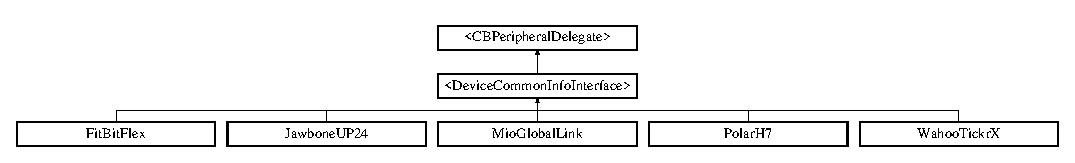
\includegraphics[height=2.176166cm]{protocol_device_common_info_interface-p}
\end{center}
\end{figure}
\subsection*{Instance Methods}
\begin{DoxyCompactItemize}
\item 
(id$<$ \hyperlink{protocol_device_common_info_interface-p}{Device\-Common\-Info\-Interface} $>$) -\/ \hyperlink{protocol_device_common_info_interface-p_ac0680a5ceb7f913c49598eeda2dad07c}{init\-With\-Peripheral\-:}
\item 
(B\-O\-O\-L) -\/ \hyperlink{protocol_device_common_info_interface-p_a5a149dfb93c5c7a364460d8df26537b2}{is\-Connected}
\item 
(int) -\/ \hyperlink{protocol_device_common_info_interface-p_a54b8e239d2d0470be0d906b11b7f3850}{battery\-Level}
\item 
(void) -\/ \hyperlink{protocol_device_common_info_interface-p_a3e95f2da7a5916c8bb6d9b6b76fac3e7}{discover\-Battery\-Level}
\item 
(N\-S\-Integer) -\/ \hyperlink{protocol_device_common_info_interface-p_a2817a747a1ab2cf6f199b1cebe86bd83}{type}
\item 
(void) -\/ \hyperlink{protocol_device_common_info_interface-p_a1fa243ee7ba284b691c365bae4f9b463}{set\-Type\-:}
\item 
(N\-S\-String $\ast$) -\/ \hyperlink{protocol_device_common_info_interface-p_a4ae9cbc86f48df7167b691e91984f266}{name}
\item 
(C\-B\-Peripheral $\ast$) -\/ \hyperlink{protocol_device_common_info_interface-p_a60acee2f42fa42a04ba3585e08d75f8e}{device}
\item 
(void) -\/ \hyperlink{protocol_device_common_info_interface-p_a64200062c5687034c8e2ef6dd83bba0f}{get\-Table\-Information}
\item 
(void) -\/ \hyperlink{protocol_device_common_info_interface-p_a9d3d278049f74d785a57ed2aecf22e22}{should\-Monitor\-:}
\item 
(B\-O\-O\-L) -\/ \hyperlink{protocol_device_common_info_interface-p_a83c3e03ff34cc8b954743a76d77facea}{discovery\-Complete}
\item 
(N\-S\-String $\ast$) -\/ \hyperlink{protocol_device_common_info_interface-p_a4fa63c9f7fe49ddaa32bd40159bc7a8c}{manufacturer}
\end{DoxyCompactItemize}


\subsection{Detailed Description}
This protocol is created to make an A\-P\-I for the devices so that similar operations can be performed. All of the devices are C\-B\-Peripheral devices. They have different U\-U\-I\-Ds for their services and differing characteristics, so their interactions are different. This A\-P\-I is an attempt to hide the complexity for the sake of brevity in the code and to make things more readable elsewhere. Device specific operations are done in the class files associated with the devices. 

\subsection{Method Documentation}
\hypertarget{protocol_device_common_info_interface-p_a54b8e239d2d0470be0d906b11b7f3850}{\index{Device\-Common\-Info\-Interface-\/p@{Device\-Common\-Info\-Interface-\/p}!battery\-Level@{battery\-Level}}
\index{battery\-Level@{battery\-Level}!DeviceCommonInfoInterface-p@{Device\-Common\-Info\-Interface-\/p}}
\subsubsection[{battery\-Level}]{\setlength{\rightskip}{0pt plus 5cm}-\/ (int) battery\-Level 
\begin{DoxyParamCaption}
{}
\end{DoxyParamCaption}
\hspace{0.3cm}{\ttfamily [required]}}}\label{protocol_device_common_info_interface-p_a54b8e239d2d0470be0d906b11b7f3850}
This method retrieves the battery level as expressed as a percent integer. It assumed that a update\-Battery\-Level call was made, otherwise the last known value is returned.

\begin{DoxyReturn}{Returns}
N\-S\-Integer value from 0 to 100 expressing the percent of charge. 0 is default for unread or unreadable battery level characteristic. 
\end{DoxyReturn}
\hypertarget{protocol_device_common_info_interface-p_a60acee2f42fa42a04ba3585e08d75f8e}{\index{Device\-Common\-Info\-Interface-\/p@{Device\-Common\-Info\-Interface-\/p}!device@{device}}
\index{device@{device}!DeviceCommonInfoInterface-p@{Device\-Common\-Info\-Interface-\/p}}
\subsubsection[{device}]{\setlength{\rightskip}{0pt plus 5cm}-\/ (C\-B\-Peripheral$\ast$) device 
\begin{DoxyParamCaption}
{}
\end{DoxyParamCaption}
\hspace{0.3cm}{\ttfamily [required]}}}\label{protocol_device_common_info_interface-p_a60acee2f42fa42a04ba3585e08d75f8e}
This method returns the actual C\-B\-Peripheral device for use with the device manager in order to manage connectivity to the device. This object is immutable and does not have any write characteristics. \hypertarget{protocol_device_common_info_interface-p_a3e95f2da7a5916c8bb6d9b6b76fac3e7}{\index{Device\-Common\-Info\-Interface-\/p@{Device\-Common\-Info\-Interface-\/p}!discover\-Battery\-Level@{discover\-Battery\-Level}}
\index{discover\-Battery\-Level@{discover\-Battery\-Level}!DeviceCommonInfoInterface-p@{Device\-Common\-Info\-Interface-\/p}}
\subsubsection[{discover\-Battery\-Level}]{\setlength{\rightskip}{0pt plus 5cm}-\/ (void) discover\-Battery\-Level 
\begin{DoxyParamCaption}
{}
\end{DoxyParamCaption}
\hspace{0.3cm}{\ttfamily [required]}}}\label{protocol_device_common_info_interface-p_a3e95f2da7a5916c8bb6d9b6b76fac3e7}
This method forces the device to read and broadcast the battery level. \hypertarget{protocol_device_common_info_interface-p_a83c3e03ff34cc8b954743a76d77facea}{\index{Device\-Common\-Info\-Interface-\/p@{Device\-Common\-Info\-Interface-\/p}!discovery\-Complete@{discovery\-Complete}}
\index{discovery\-Complete@{discovery\-Complete}!DeviceCommonInfoInterface-p@{Device\-Common\-Info\-Interface-\/p}}
\subsubsection[{discovery\-Complete}]{\setlength{\rightskip}{0pt plus 5cm}-\/ (B\-O\-O\-L) discovery\-Complete 
\begin{DoxyParamCaption}
{}
\end{DoxyParamCaption}
\hspace{0.3cm}{\ttfamily [required]}}}\label{protocol_device_common_info_interface-p_a83c3e03ff34cc8b954743a76d77facea}
This method is used to prevent premature interruption of discovery scan.

\begin{DoxyReturn}{Returns}
Y\-E\-S if all of the services for this device have been discovered. 
\end{DoxyReturn}
\hypertarget{protocol_device_common_info_interface-p_a64200062c5687034c8e2ef6dd83bba0f}{\index{Device\-Common\-Info\-Interface-\/p@{Device\-Common\-Info\-Interface-\/p}!get\-Table\-Information@{get\-Table\-Information}}
\index{get\-Table\-Information@{get\-Table\-Information}!DeviceCommonInfoInterface-p@{Device\-Common\-Info\-Interface-\/p}}
\subsubsection[{get\-Table\-Information}]{\setlength{\rightskip}{0pt plus 5cm}-\/ (void) get\-Table\-Information 
\begin{DoxyParamCaption}
{}
\end{DoxyParamCaption}
\hspace{0.3cm}{\ttfamily [required]}}}\label{protocol_device_common_info_interface-p_a64200062c5687034c8e2ef6dd83bba0f}
This method forces queries of the device in order to get the applicable data for this device. \hypertarget{protocol_device_common_info_interface-p_ac0680a5ceb7f913c49598eeda2dad07c}{\index{Device\-Common\-Info\-Interface-\/p@{Device\-Common\-Info\-Interface-\/p}!init\-With\-Peripheral\-:@{init\-With\-Peripheral\-:}}
\index{init\-With\-Peripheral\-:@{init\-With\-Peripheral\-:}!DeviceCommonInfoInterface-p@{Device\-Common\-Info\-Interface-\/p}}
\subsubsection[{init\-With\-Peripheral\-:}]{\setlength{\rightskip}{0pt plus 5cm}-\/ (id$<${\bf Device\-Common\-Info\-Interface}$>$) init\-With\-Peripheral\-: 
\begin{DoxyParamCaption}
\item[{(C\-B\-Peripheral $\ast$)}]{peripheral}
\end{DoxyParamCaption}
\hspace{0.3cm}{\ttfamily [required]}}}\label{protocol_device_common_info_interface-p_ac0680a5ceb7f913c49598eeda2dad07c}
This initialization method creates the desired device based on the C\-B\-Peripheral that is discovered. It is common to all types of devices and will bypass use of the standard init method for those classes. This method is used by the \hyperlink{interface_monitor_creation_factory}{Monitor\-Creation\-Factory} as a standard for initializing the device and providing all of the methods in this protocol.


\begin{DoxyParams}{Parameters}
{\em C\-B\-Peripheral} & is the device object that the C\-B\-Central\-Manager discovered. \\
\hline
\end{DoxyParams}
\begin{DoxyReturn}{Returns}
id$<$\-Device\-Common\-Info\-Interface$>$ This object is any class that conforms to the \hyperlink{protocol_device_common_info_interface-p}{Device\-Common\-Info\-Interface} protocol. 
\end{DoxyReturn}
\hypertarget{protocol_device_common_info_interface-p_a5a149dfb93c5c7a364460d8df26537b2}{\index{Device\-Common\-Info\-Interface-\/p@{Device\-Common\-Info\-Interface-\/p}!is\-Connected@{is\-Connected}}
\index{is\-Connected@{is\-Connected}!DeviceCommonInfoInterface-p@{Device\-Common\-Info\-Interface-\/p}}
\subsubsection[{is\-Connected}]{\setlength{\rightskip}{0pt plus 5cm}-\/ (B\-O\-O\-L) is\-Connected 
\begin{DoxyParamCaption}
{}
\end{DoxyParamCaption}
\hspace{0.3cm}{\ttfamily [required]}}}\label{protocol_device_common_info_interface-p_a5a149dfb93c5c7a364460d8df26537b2}
This method does a check to see if the the device is actually connected and returns a value of T\-R\-U\-E if it is currently connected. If the Device is in any other state, the return value is F\-A\-L\-S\-E.

\begin{DoxyReturn}{Returns}
T\-R\-U\-E or F\-A\-L\-S\-E value if the device is connected. 
\end{DoxyReturn}
\hypertarget{protocol_device_common_info_interface-p_a4fa63c9f7fe49ddaa32bd40159bc7a8c}{\index{Device\-Common\-Info\-Interface-\/p@{Device\-Common\-Info\-Interface-\/p}!manufacturer@{manufacturer}}
\index{manufacturer@{manufacturer}!DeviceCommonInfoInterface-p@{Device\-Common\-Info\-Interface-\/p}}
\subsubsection[{manufacturer}]{\setlength{\rightskip}{0pt plus 5cm}-\/ (N\-S\-String$\ast$) manufacturer 
\begin{DoxyParamCaption}
{}
\end{DoxyParamCaption}
\hspace{0.3cm}{\ttfamily [optional]}}}\label{protocol_device_common_info_interface-p_a4fa63c9f7fe49ddaa32bd40159bc7a8c}
This method is used to fill in details in the discovery view table. It is optional.

\begin{DoxyReturn}{Returns}
This N\-S\-String value that the device broadcast for the manufacturer name in the Device Information characteristic. Not all devices have this information. 
\end{DoxyReturn}
\hypertarget{protocol_device_common_info_interface-p_a4ae9cbc86f48df7167b691e91984f266}{\index{Device\-Common\-Info\-Interface-\/p@{Device\-Common\-Info\-Interface-\/p}!name@{name}}
\index{name@{name}!DeviceCommonInfoInterface-p@{Device\-Common\-Info\-Interface-\/p}}
\subsubsection[{name}]{\setlength{\rightskip}{0pt plus 5cm}-\/ (N\-S\-String$\ast$) name 
\begin{DoxyParamCaption}
{}
\end{DoxyParamCaption}
\hspace{0.3cm}{\ttfamily [required]}}}\label{protocol_device_common_info_interface-p_a4ae9cbc86f48df7167b691e91984f266}
Returns the device name of the C\-B\-Peripheral that is in the class of the object. Created for easy reading and consist access.

\begin{DoxyReturn}{Returns}
an N\-S\-String of the device name. 
\end{DoxyReturn}
\hypertarget{protocol_device_common_info_interface-p_a1fa243ee7ba284b691c365bae4f9b463}{\index{Device\-Common\-Info\-Interface-\/p@{Device\-Common\-Info\-Interface-\/p}!set\-Type\-:@{set\-Type\-:}}
\index{set\-Type\-:@{set\-Type\-:}!DeviceCommonInfoInterface-p@{Device\-Common\-Info\-Interface-\/p}}
\subsubsection[{set\-Type\-:}]{\setlength{\rightskip}{0pt plus 5cm}-\/ (void) set\-Type\-: 
\begin{DoxyParamCaption}
\item[{(N\-S\-Integer)}]{type}
\end{DoxyParamCaption}
\hspace{0.3cm}{\ttfamily [required]}}}\label{protocol_device_common_info_interface-p_a1fa243ee7ba284b691c365bae4f9b463}
This sets the device type so that the device can be easily placed in the desired array of the controller.


\begin{DoxyParams}{Parameters}
{\em type} & is the N\-S\-Integer defined from the \hyperlink{_device_types_8h_source}{Device\-Types.\-h} file. This field is used to help determine if a device belongs in the heart monitors array or the activity monitors array. \\
\hline
\end{DoxyParams}
\hypertarget{protocol_device_common_info_interface-p_a9d3d278049f74d785a57ed2aecf22e22}{\index{Device\-Common\-Info\-Interface-\/p@{Device\-Common\-Info\-Interface-\/p}!should\-Monitor\-:@{should\-Monitor\-:}}
\index{should\-Monitor\-:@{should\-Monitor\-:}!DeviceCommonInfoInterface-p@{Device\-Common\-Info\-Interface-\/p}}
\subsubsection[{should\-Monitor\-:}]{\setlength{\rightskip}{0pt plus 5cm}-\/ (void) should\-Monitor\-: 
\begin{DoxyParamCaption}
\item[{(B\-O\-O\-L)}]{monitor}
\end{DoxyParamCaption}
\hspace{0.3cm}{\ttfamily [required]}}}\label{protocol_device_common_info_interface-p_a9d3d278049f74d785a57ed2aecf22e22}
This method is used to toggle monitoring because the devices can have setup and teardown procedures. 
\begin{DoxyParams}{Parameters}
{\em monitor} & The state to decide whether to start monitoring or not. \\
\hline
\end{DoxyParams}
\hypertarget{protocol_device_common_info_interface-p_a2817a747a1ab2cf6f199b1cebe86bd83}{\index{Device\-Common\-Info\-Interface-\/p@{Device\-Common\-Info\-Interface-\/p}!type@{type}}
\index{type@{type}!DeviceCommonInfoInterface-p@{Device\-Common\-Info\-Interface-\/p}}
\subsubsection[{type}]{\setlength{\rightskip}{0pt plus 5cm}-\/ (N\-S\-Integer) type 
\begin{DoxyParamCaption}
{}
\end{DoxyParamCaption}
\hspace{0.3cm}{\ttfamily [required]}}}\label{protocol_device_common_info_interface-p_a2817a747a1ab2cf6f199b1cebe86bd83}
This method returns the device type. It is used for a shallow query of the object so that it can be placed in correct array of the bluetooth manager. See \hyperlink{_device_types_8h_source}{Device\-Types.\-h} for the values.

\begin{DoxyReturn}{Returns}
Returns an N\-S\-Integer that fits within the confines of the \hyperlink{_device_types_8h_source}{Device\-Types.\-h} file. 
\end{DoxyReturn}


The documentation for this protocol was generated from the following file\-:\begin{DoxyCompactItemize}
\item 
Device\-Common\-Info\-Interface.\-h\end{DoxyCompactItemize}

\hypertarget{class_device_constants_and_static_functions}{\section{Device\-Constants\-And\-Static\-Functions Class Reference}
\label{class_device_constants_and_static_functions}\index{Device\-Constants\-And\-Static\-Functions@{Device\-Constants\-And\-Static\-Functions}}
}


The documentation for this class was generated from the following file\-:\begin{DoxyCompactItemize}
\item 
/\-Users/douglas/\-Documents/software/\-Senior Project/ios/\-Medical Cyborgs/\-Medical Cyborgs/Device\-Constants\-And\-Static\-Functions.\-m\end{DoxyCompactItemize}

\hypertarget{interface_device_poll_manager}{\section{Device\-Poll\-Manager Class Reference}
\label{interface_device_poll_manager}\index{Device\-Poll\-Manager@{Device\-Poll\-Manager}}
}


{\ttfamily \#import $<$Device\-Poll\-Manager.\-h$>$}

Inheritance diagram for Device\-Poll\-Manager\-:\begin{figure}[H]
\begin{center}
\leavevmode
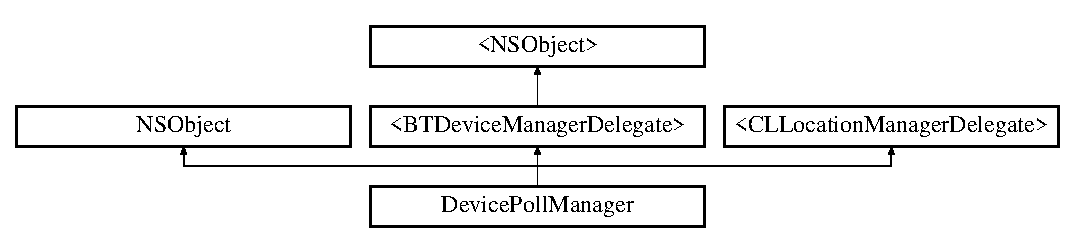
\includegraphics[height=2.814070cm]{interface_device_poll_manager}
\end{center}
\end{figure}
\subsection*{Instance Methods}
\begin{DoxyCompactItemize}
\item 
(U\-I\-Application $\ast$) -\/ \hyperlink{interface_device_poll_manager_a896832635ddcf3d3d1f60cd856f0dd96}{app}
\item 
(id) -\/ \hyperlink{interface_device_poll_manager_ac1637206b4271575f8b2afd39375125b}{init\-With\-Data\-Store\-:and\-Devicemanager\-:}
\item 
(void) -\/ \hyperlink{interface_device_poll_manager_ac0c31de4251c9eac9b21594cc866f165}{poll\-Devices\-For\-Data}
\item 
(void) -\/ \hyperlink{interface_device_poll_manager_a91b7db2f338c98f0d653e8a33d95b736}{did\-Receive\-Notification\-Device\-Connected}
\item 
(void) -\/ \hyperlink{interface_device_poll_manager_a4fe6160b06d23999e8939c88e900b232}{stop\-Monitoring}
\item 
(void) -\/ \hyperlink{interface_device_poll_manager_aa0e15e54081df4d481de96cde113f2b8}{do\-Battery\-Low\-Notification\-For\-:}
\end{DoxyCompactItemize}
\subsection*{Properties}
\begin{DoxyCompactItemize}
\item 
B\-O\-O\-L \hyperlink{interface_device_poll_manager_a265079b7aa0e9cc69818fb49835bd175}{low\-Battery\-Notified}
\item 
C\-L\-Location\-Manager $\ast$ \hyperlink{interface_device_poll_manager_ad710c38392bfc32d3509de470e0cfa8d}{location\-Manager}
\item 
B\-O\-O\-L \hyperlink{interface_device_poll_manager_a0e9aad6cc4f5a99aff27b0a64ae76d19}{location\-Allowed}
\item 
\hyperlink{interface_personal_info}{Personal\-Info} $\ast$ \hyperlink{interface_device_poll_manager_a8739ffcaa2b1e02afc1864e338de148f}{patient\-Info}
\item 
N\-S\-Integer \hyperlink{interface_device_poll_manager_a621e3962372201145248997e2eb87327}{patient\-I\-D}
\item 
\hyperlink{interface_b_t_device_manager}{B\-T\-Device\-Manager} $\ast$ \hyperlink{interface_device_poll_manager_a813e014763804b71e247ca335fe91761}{device\-Manager}
\item 
id$<$ \hyperlink{protocol_device_common_info_interface-p}{Device\-Common\-Info\-Interface}, \\*
\hyperlink{protocol_heart_monitor_protocol-p}{Heart\-Monitor\-Protocol} $>$ \hyperlink{interface_device_poll_manager_a5d06bcab588b72afdf5fce4c102afe91}{heart\-Monitor}
\item 
id$<$ \hyperlink{protocol_device_common_info_interface-p}{Device\-Common\-Info\-Interface}, \\*
\hyperlink{protocol_activity_monitor_protocol-p}{Activity\-Monitor\-Protocol} $>$ \hyperlink{interface_device_poll_manager_a1e33e8f7da83c22dccb6c3b3b7d66069}{activity\-Monitor}
\item 
\hyperlink{interface_d_b_manager}{D\-B\-Manager} $\ast$ \hyperlink{interface_device_poll_manager_a66a02f95a478a42c7e45986317e3c6c1}{database}
\item 
B\-O\-O\-L \hyperlink{interface_device_poll_manager_a8d5b5ff2c336f0dd2cb2b9e088850072}{battery\-Alert\-Given}
\item 
B\-O\-O\-L \hyperlink{interface_device_poll_manager_abe71cba97ae5b0faef77e70b78f2bef2}{able\-To\-Poll}
\item 
B\-O\-O\-L \hyperlink{interface_device_poll_manager_a4735e7c0b634e8693ac8d33a0456d39f}{is\-Heart\-Monitor\-Ready}
\item 
B\-O\-O\-L \hyperlink{interface_device_poll_manager_aeab69bf0530fcf7d3f1b01c785e17bd2}{is\-Activity\-Monitor\-Ready}
\item 
int \hyperlink{interface_device_poll_manager_a302b6434aa606031f78f721c9e40f0cf}{current\-Heart\-Rate}
\end{DoxyCompactItemize}


\subsection{Detailed Description}
This class functions as the polling mechanism for the bluetooth devices. Its goes through each time the main method is called and retrieves the information from the devices and puts the data in the local data store. 

\subsection{Method Documentation}
\hypertarget{interface_device_poll_manager_a896832635ddcf3d3d1f60cd856f0dd96}{\index{Device\-Poll\-Manager@{Device\-Poll\-Manager}!app@{app}}
\index{app@{app}!DevicePollManager@{Device\-Poll\-Manager}}
\subsubsection[{app}]{\setlength{\rightskip}{0pt plus 5cm}-\/ (U\-I\-Application $\ast$) app 
\begin{DoxyParamCaption}
{}
\end{DoxyParamCaption}
}}\label{interface_device_poll_manager_a896832635ddcf3d3d1f60cd856f0dd96}
This method returns the shared instance of the application. \hypertarget{interface_device_poll_manager_a91b7db2f338c98f0d653e8a33d95b736}{\index{Device\-Poll\-Manager@{Device\-Poll\-Manager}!did\-Receive\-Notification\-Device\-Connected@{did\-Receive\-Notification\-Device\-Connected}}
\index{did\-Receive\-Notification\-Device\-Connected@{did\-Receive\-Notification\-Device\-Connected}!DevicePollManager@{Device\-Poll\-Manager}}
\subsubsection[{did\-Receive\-Notification\-Device\-Connected}]{\setlength{\rightskip}{0pt plus 5cm}-\/ (void) did\-Receive\-Notification\-Device\-Connected 
\begin{DoxyParamCaption}
{}
\end{DoxyParamCaption}
}}\label{interface_device_poll_manager_a91b7db2f338c98f0d653e8a33d95b736}
This method is used by the device manager to notify the poller that a device is connected. It is used to help signal the device poller that it can continue because all devices are connected. \hypertarget{interface_device_poll_manager_aa0e15e54081df4d481de96cde113f2b8}{\index{Device\-Poll\-Manager@{Device\-Poll\-Manager}!do\-Battery\-Low\-Notification\-For\-:@{do\-Battery\-Low\-Notification\-For\-:}}
\index{do\-Battery\-Low\-Notification\-For\-:@{do\-Battery\-Low\-Notification\-For\-:}!DevicePollManager@{Device\-Poll\-Manager}}
\subsubsection[{do\-Battery\-Low\-Notification\-For\-:}]{\setlength{\rightskip}{0pt plus 5cm}-\/ (void) do\-Battery\-Low\-Notification\-For\-: 
\begin{DoxyParamCaption}
\item[{(id$<${\bf Device\-Common\-Info\-Interface}$>$)}]{device}
\end{DoxyParamCaption}
}}\label{interface_device_poll_manager_aa0e15e54081df4d481de96cde113f2b8}
This method pushes notifications that the battery is low for one of the devices.


\begin{DoxyParams}{Parameters}
{\em device} & The bluetooth device that is low on battery. \\
\hline
\end{DoxyParams}
\hypertarget{interface_device_poll_manager_ac1637206b4271575f8b2afd39375125b}{\index{Device\-Poll\-Manager@{Device\-Poll\-Manager}!init\-With\-Data\-Store\-:and\-Devicemanager\-:@{init\-With\-Data\-Store\-:and\-Devicemanager\-:}}
\index{init\-With\-Data\-Store\-:and\-Devicemanager\-:@{init\-With\-Data\-Store\-:and\-Devicemanager\-:}!DevicePollManager@{Device\-Poll\-Manager}}
\subsubsection[{init\-With\-Data\-Store\-:and\-Devicemanager\-:}]{\setlength{\rightskip}{0pt plus 5cm}-\/ (id) init\-With\-Data\-Store\-: 
\begin{DoxyParamCaption}
\item[{({\bf D\-B\-Manager}$\ast$)}]{data\-Store}
\item[{andDevicemanager:({\bf B\-T\-Device\-Manager}$\ast$)}]{new\-Device\-Manager}
\end{DoxyParamCaption}
}}\label{interface_device_poll_manager_ac1637206b4271575f8b2afd39375125b}
This is the preferred initialization method. The datastore and the two components are passed so that polling can happen imediately. W\-A\-R\-N\-I\-N\-G\-: This initialization method must be used if any polling is to occur.


\begin{DoxyParams}{Parameters}
{\em data\-Store} & The database manager that will be used for local storage of the data.\\
\hline
{\em new\-Device\-Manager} & The device manager that is to maintain the connectivity of the devices.\\
\hline
\end{DoxyParams}
\begin{DoxyReturn}{Returns}
An instance of the device poller which contains everything that is needed to run. 
\end{DoxyReturn}
\hypertarget{interface_device_poll_manager_ac0c31de4251c9eac9b21594cc866f165}{\index{Device\-Poll\-Manager@{Device\-Poll\-Manager}!poll\-Devices\-For\-Data@{poll\-Devices\-For\-Data}}
\index{poll\-Devices\-For\-Data@{poll\-Devices\-For\-Data}!DevicePollManager@{Device\-Poll\-Manager}}
\subsubsection[{poll\-Devices\-For\-Data}]{\setlength{\rightskip}{0pt plus 5cm}-\/ (void) poll\-Devices\-For\-Data 
\begin{DoxyParamCaption}
{}
\end{DoxyParamCaption}
}}\label{interface_device_poll_manager_ac0c31de4251c9eac9b21594cc866f165}
This method is used to get information from the devices. If the devices have not been added with the init\-With\-Data\-Store\-: heart\-Monitor\-: activity\-Monitor\-: no updates will occur. The appropriate data is pulled from the devices for monitoring. The battery level, if readable is also polled. If the battery is below 20\% a notification will be posted to the N\-S\-Notification\-Center. \hypertarget{interface_device_poll_manager_a4fe6160b06d23999e8939c88e900b232}{\index{Device\-Poll\-Manager@{Device\-Poll\-Manager}!stop\-Monitoring@{stop\-Monitoring}}
\index{stop\-Monitoring@{stop\-Monitoring}!DevicePollManager@{Device\-Poll\-Manager}}
\subsubsection[{stop\-Monitoring}]{\setlength{\rightskip}{0pt plus 5cm}-\/ (void) stop\-Monitoring 
\begin{DoxyParamCaption}
{}
\end{DoxyParamCaption}
}}\label{interface_device_poll_manager_a4fe6160b06d23999e8939c88e900b232}
This method is used to tell the device poller to stop monitoring the selected monitors. 

\subsection{Property Documentation}
\hypertarget{interface_device_poll_manager_abe71cba97ae5b0faef77e70b78f2bef2}{\index{Device\-Poll\-Manager@{Device\-Poll\-Manager}!able\-To\-Poll@{able\-To\-Poll}}
\index{able\-To\-Poll@{able\-To\-Poll}!DevicePollManager@{Device\-Poll\-Manager}}
\subsubsection[{able\-To\-Poll}]{\setlength{\rightskip}{0pt plus 5cm}-\/ (B\-O\-O\-L) able\-To\-Poll\hspace{0.3cm}{\ttfamily [read]}, {\ttfamily [write]}, {\ttfamily [atomic]}}}\label{interface_device_poll_manager_abe71cba97ae5b0faef77e70b78f2bef2}
This flag determines whether polling will continue. This can be F\-A\-L\-S\-E when the following conditions exist. Either of the devices is not connected. The devices has not been fully discovered. \hypertarget{interface_device_poll_manager_a1e33e8f7da83c22dccb6c3b3b7d66069}{\index{Device\-Poll\-Manager@{Device\-Poll\-Manager}!activity\-Monitor@{activity\-Monitor}}
\index{activity\-Monitor@{activity\-Monitor}!DevicePollManager@{Device\-Poll\-Manager}}
\subsubsection[{activity\-Monitor}]{\setlength{\rightskip}{0pt plus 5cm}-\/ (id$<${\bf Device\-Common\-Info\-Interface}, {\bf Activity\-Monitor\-Protocol}$>$) activity\-Monitor\hspace{0.3cm}{\ttfamily [read]}, {\ttfamily [write]}, {\ttfamily [atomic]}}}\label{interface_device_poll_manager_a1e33e8f7da83c22dccb6c3b3b7d66069}
The activity monitor that was selected. The reference is used for code brevity. \hypertarget{interface_device_poll_manager_a8d5b5ff2c336f0dd2cb2b9e088850072}{\index{Device\-Poll\-Manager@{Device\-Poll\-Manager}!battery\-Alert\-Given@{battery\-Alert\-Given}}
\index{battery\-Alert\-Given@{battery\-Alert\-Given}!DevicePollManager@{Device\-Poll\-Manager}}
\subsubsection[{battery\-Alert\-Given}]{\setlength{\rightskip}{0pt plus 5cm}-\/ (B\-O\-O\-L) battery\-Alert\-Given\hspace{0.3cm}{\ttfamily [read]}, {\ttfamily [write]}, {\ttfamily [atomic]}}}\label{interface_device_poll_manager_a8d5b5ff2c336f0dd2cb2b9e088850072}
This flag is set once a low battery indication has happened. The default for the battery alert is 20\% of battery left on one of the devices. \hypertarget{interface_device_poll_manager_a302b6434aa606031f78f721c9e40f0cf}{\index{Device\-Poll\-Manager@{Device\-Poll\-Manager}!current\-Heart\-Rate@{current\-Heart\-Rate}}
\index{current\-Heart\-Rate@{current\-Heart\-Rate}!DevicePollManager@{Device\-Poll\-Manager}}
\subsubsection[{current\-Heart\-Rate}]{\setlength{\rightskip}{0pt plus 5cm}-\/ (int) current\-Heart\-Rate\hspace{0.3cm}{\ttfamily [read]}, {\ttfamily [write]}, {\ttfamily [atomic]}}}\label{interface_device_poll_manager_a302b6434aa606031f78f721c9e40f0cf}
The current heart rate. It will be 0 if no heart rate has been detected, or it will stay at the last value if the heart rate monitor is lost. \hypertarget{interface_device_poll_manager_a66a02f95a478a42c7e45986317e3c6c1}{\index{Device\-Poll\-Manager@{Device\-Poll\-Manager}!database@{database}}
\index{database@{database}!DevicePollManager@{Device\-Poll\-Manager}}
\subsubsection[{database}]{\setlength{\rightskip}{0pt plus 5cm}-\/ ({\bf D\-B\-Manager}$\ast$) database\hspace{0.3cm}{\ttfamily [read]}, {\ttfamily [write]}, {\ttfamily [atomic]}}}\label{interface_device_poll_manager_a66a02f95a478a42c7e45986317e3c6c1}
The local database that will be used for storage of the data retrieved from the devices during polling. \hypertarget{interface_device_poll_manager_a813e014763804b71e247ca335fe91761}{\index{Device\-Poll\-Manager@{Device\-Poll\-Manager}!device\-Manager@{device\-Manager}}
\index{device\-Manager@{device\-Manager}!DevicePollManager@{Device\-Poll\-Manager}}
\subsubsection[{device\-Manager}]{\setlength{\rightskip}{0pt plus 5cm}-\/ ({\bf B\-T\-Device\-Manager}$\ast$) device\-Manager\hspace{0.3cm}{\ttfamily [read]}, {\ttfamily [write]}, {\ttfamily [atomic]}, {\ttfamily [retain]}}}\label{interface_device_poll_manager_a813e014763804b71e247ca335fe91761}
The device manager which controls connectivity to the devices. \hypertarget{interface_device_poll_manager_a5d06bcab588b72afdf5fce4c102afe91}{\index{Device\-Poll\-Manager@{Device\-Poll\-Manager}!heart\-Monitor@{heart\-Monitor}}
\index{heart\-Monitor@{heart\-Monitor}!DevicePollManager@{Device\-Poll\-Manager}}
\subsubsection[{heart\-Monitor}]{\setlength{\rightskip}{0pt plus 5cm}-\/ (id$<${\bf Device\-Common\-Info\-Interface}, {\bf Heart\-Monitor\-Protocol}$>$) heart\-Monitor\hspace{0.3cm}{\ttfamily [read]}, {\ttfamily [write]}, {\ttfamily [atomic]}}}\label{interface_device_poll_manager_a5d06bcab588b72afdf5fce4c102afe91}
The heart monitor that was selected. This reference is used for code brevity. \hypertarget{interface_device_poll_manager_aeab69bf0530fcf7d3f1b01c785e17bd2}{\index{Device\-Poll\-Manager@{Device\-Poll\-Manager}!is\-Activity\-Monitor\-Ready@{is\-Activity\-Monitor\-Ready}}
\index{is\-Activity\-Monitor\-Ready@{is\-Activity\-Monitor\-Ready}!DevicePollManager@{Device\-Poll\-Manager}}
\subsubsection[{is\-Activity\-Monitor\-Ready}]{\setlength{\rightskip}{0pt plus 5cm}-\/ (B\-O\-O\-L) is\-Activity\-Monitor\-Ready\hspace{0.3cm}{\ttfamily [read]}, {\ttfamily [write]}, {\ttfamily [atomic]}}}\label{interface_device_poll_manager_aeab69bf0530fcf7d3f1b01c785e17bd2}
This flag is set when the activity monitor is connected and fully discovered. \hypertarget{interface_device_poll_manager_a4735e7c0b634e8693ac8d33a0456d39f}{\index{Device\-Poll\-Manager@{Device\-Poll\-Manager}!is\-Heart\-Monitor\-Ready@{is\-Heart\-Monitor\-Ready}}
\index{is\-Heart\-Monitor\-Ready@{is\-Heart\-Monitor\-Ready}!DevicePollManager@{Device\-Poll\-Manager}}
\subsubsection[{is\-Heart\-Monitor\-Ready}]{\setlength{\rightskip}{0pt plus 5cm}-\/ (B\-O\-O\-L) is\-Heart\-Monitor\-Ready\hspace{0.3cm}{\ttfamily [read]}, {\ttfamily [write]}, {\ttfamily [atomic]}}}\label{interface_device_poll_manager_a4735e7c0b634e8693ac8d33a0456d39f}
This flag is set when the heart monitor is connected and activity monitor are fully discovered. \hypertarget{interface_device_poll_manager_a0e9aad6cc4f5a99aff27b0a64ae76d19}{\index{Device\-Poll\-Manager@{Device\-Poll\-Manager}!location\-Allowed@{location\-Allowed}}
\index{location\-Allowed@{location\-Allowed}!DevicePollManager@{Device\-Poll\-Manager}}
\subsubsection[{location\-Allowed}]{\setlength{\rightskip}{0pt plus 5cm}-\/ (B\-O\-O\-L) location\-Allowed\hspace{0.3cm}{\ttfamily [read]}, {\ttfamily [write]}, {\ttfamily [atomic]}}}\label{interface_device_poll_manager_a0e9aad6cc4f5a99aff27b0a64ae76d19}
The flag that is used for checking to see if any location checks are allowed by the user. \hypertarget{interface_device_poll_manager_ad710c38392bfc32d3509de470e0cfa8d}{\index{Device\-Poll\-Manager@{Device\-Poll\-Manager}!location\-Manager@{location\-Manager}}
\index{location\-Manager@{location\-Manager}!DevicePollManager@{Device\-Poll\-Manager}}
\subsubsection[{location\-Manager}]{\setlength{\rightskip}{0pt plus 5cm}-\/ (C\-L\-Location\-Manager$\ast$) location\-Manager\hspace{0.3cm}{\ttfamily [read]}, {\ttfamily [write]}, {\ttfamily [atomic]}, {\ttfamily [strong]}}}\label{interface_device_poll_manager_ad710c38392bfc32d3509de470e0cfa8d}
The location manager used for tracking the location of the patient for large updates. \hypertarget{interface_device_poll_manager_a265079b7aa0e9cc69818fb49835bd175}{\index{Device\-Poll\-Manager@{Device\-Poll\-Manager}!low\-Battery\-Notified@{low\-Battery\-Notified}}
\index{low\-Battery\-Notified@{low\-Battery\-Notified}!DevicePollManager@{Device\-Poll\-Manager}}
\subsubsection[{low\-Battery\-Notified}]{\setlength{\rightskip}{0pt plus 5cm}-\/ (B\-O\-O\-L) low\-Battery\-Notified\hspace{0.3cm}{\ttfamily [read]}, {\ttfamily [write]}, {\ttfamily [atomic]}}}\label{interface_device_poll_manager_a265079b7aa0e9cc69818fb49835bd175}
flag to represent that the low battery notification has been done. \hypertarget{interface_device_poll_manager_a621e3962372201145248997e2eb87327}{\index{Device\-Poll\-Manager@{Device\-Poll\-Manager}!patient\-I\-D@{patient\-I\-D}}
\index{patient\-I\-D@{patient\-I\-D}!DevicePollManager@{Device\-Poll\-Manager}}
\subsubsection[{patient\-I\-D}]{\setlength{\rightskip}{0pt plus 5cm}-\/ (N\-S\-Integer) patient\-I\-D\hspace{0.3cm}{\ttfamily [read]}, {\ttfamily [write]}, {\ttfamily [atomic]}}}\label{interface_device_poll_manager_a621e3962372201145248997e2eb87327}
The patient\-I\-D is used for the device poller to insert into the database. This reference is used for code brevity. \hypertarget{interface_device_poll_manager_a8739ffcaa2b1e02afc1864e338de148f}{\index{Device\-Poll\-Manager@{Device\-Poll\-Manager}!patient\-Info@{patient\-Info}}
\index{patient\-Info@{patient\-Info}!DevicePollManager@{Device\-Poll\-Manager}}
\subsubsection[{patient\-Info}]{\setlength{\rightskip}{0pt plus 5cm}-\/ ({\bf Personal\-Info}$\ast$) patient\-Info\hspace{0.3cm}{\ttfamily [read]}, {\ttfamily [write]}, {\ttfamily [atomic]}}}\label{interface_device_poll_manager_a8739ffcaa2b1e02afc1864e338de148f}
The patient information that is locally stored by the application. It is in the N\-S\-User\-Defaults so that application restores will not require any remote connection. 

The documentation for this class was generated from the following files\-:\begin{DoxyCompactItemize}
\item 
/\-Users/douglas/\-Documents/software/\-Senior Project/ios/\-Medical Cyborgs/\-Medical Cyborgs/Device\-Poll\-Manager.\-h\item 
/\-Users/douglas/\-Documents/software/\-Senior Project/ios/\-Medical Cyborgs/\-Medical Cyborgs/Device\-Poll\-Manager.\-m\end{DoxyCompactItemize}

\hypertarget{interface_fit_bit_flex}{\section{Fit\-Bit\-Flex Class Reference}
\label{interface_fit_bit_flex}\index{Fit\-Bit\-Flex@{Fit\-Bit\-Flex}}
}
Inheritance diagram for Fit\-Bit\-Flex\-:\begin{figure}[H]
\begin{center}
\leavevmode
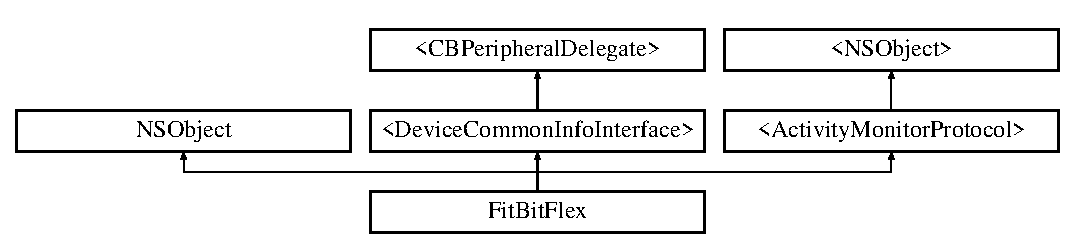
\includegraphics[height=2.901554cm]{interface_fit_bit_flex}
\end{center}
\end{figure}
\subsection*{Properties}
\begin{DoxyCompactItemize}
\item 
\hypertarget{interface_fit_bit_flex_ac539ad853d5729137679c3293cba75f5}{C\-B\-Peripheral $\ast$ {\bfseries device}}\label{interface_fit_bit_flex_ac539ad853d5729137679c3293cba75f5}

\item 
\hypertarget{interface_fit_bit_flex_af23b05b17587b9810d93909f279cca75}{C\-B\-Service $\ast$ {\bfseries battery\-Service}}\label{interface_fit_bit_flex_af23b05b17587b9810d93909f279cca75}

\item 
\hypertarget{interface_fit_bit_flex_a0d5ca990dbff1852b3d8a07faa91234b}{C\-B\-Characteristic $\ast$ {\bfseries battery\-Lvl\-Char}}\label{interface_fit_bit_flex_a0d5ca990dbff1852b3d8a07faa91234b}

\item 
\hypertarget{interface_fit_bit_flex_a6141ecb075c9553d179dc5210d2c4952}{int {\bfseries battery\-Level}}\label{interface_fit_bit_flex_a6141ecb075c9553d179dc5210d2c4952}

\item 
\hypertarget{interface_fit_bit_flex_a77895e42698dfb9e32ea3511dd68aa3e}{N\-S\-Integer {\bfseries type}}\label{interface_fit_bit_flex_a77895e42698dfb9e32ea3511dd68aa3e}

\item 
\hypertarget{interface_fit_bit_flex_a3b4fca544836750998946aab4d4c8a3d}{N\-S\-String $\ast$ {\bfseries device\-Manufacturer}}\label{interface_fit_bit_flex_a3b4fca544836750998946aab4d4c8a3d}

\end{DoxyCompactItemize}
\subsection*{Additional Inherited Members}


The documentation for this class was generated from the following files\-:\begin{DoxyCompactItemize}
\item 
/\-Users/douglas/\-Documents/software/\-Senior Project/ios/\-Medical Cyborgs/\-Medical Cyborgs/Fit\-Bit\-Flex.\-h\item 
/\-Users/douglas/\-Documents/software/\-Senior Project/ios/\-Medical Cyborgs/\-Medical Cyborgs/Fit\-Bit\-Flex.\-m\end{DoxyCompactItemize}

\hypertarget{interface_graph_v_c}{\section{Graph\-V\-C Class Reference}
\label{interface_graph_v_c}\index{Graph\-V\-C@{Graph\-V\-C}}
}


{\ttfamily \#import $<$Graph\-V\-C.\-h$>$}

Inheritance diagram for Graph\-V\-C\-:\begin{figure}[H]
\begin{center}
\leavevmode
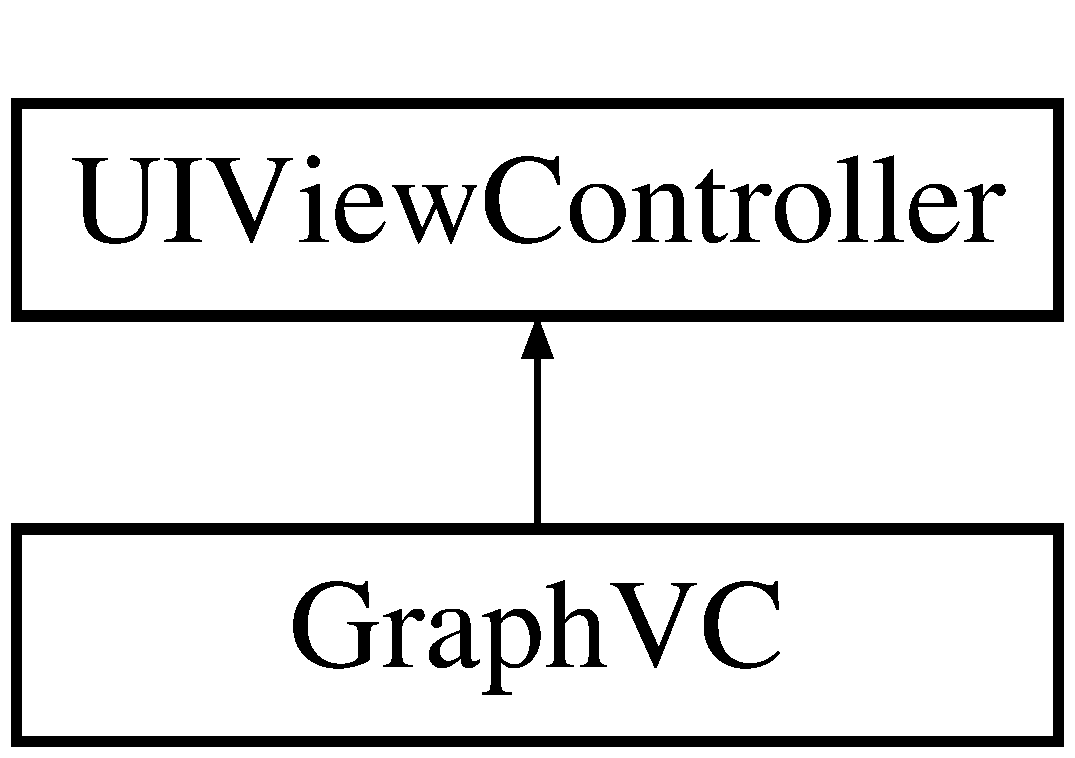
\includegraphics[height=2.000000cm]{interface_graph_v_c}
\end{center}
\end{figure}
\subsection*{Instance Methods}
\begin{DoxyCompactItemize}
\item 
(id) -\/ \hyperlink{interface_graph_v_c_ad0a240dde98905eca43bb92db53e9478}{init\-With\-Device\-Poller\-:}
\item 
(void) -\/ \hyperlink{interface_graph_v_c_a7521f143474f68142628970e9f1d7706}{update\-Display}
\end{DoxyCompactItemize}
\subsection*{Properties}
\begin{DoxyCompactItemize}
\item 
\hypertarget{interface_graph_v_c_a8a00c63cc6cab8b3c1cddaaacc9d12fc}{\hyperlink{interface_device_poll_manager}{Device\-Poll\-Manager} $\ast$ {\bfseries device\-Poller}}\label{interface_graph_v_c_a8a00c63cc6cab8b3c1cddaaacc9d12fc}

\item 
\hypertarget{interface_graph_v_c_ad434b1d838f58441c9d6499936ccd620}{I\-B\-Outlet U\-I\-Label $\ast$ {\bfseries heart\-Rate\-Display}}\label{interface_graph_v_c_ad434b1d838f58441c9d6499936ccd620}

\item 
\hypertarget{interface_graph_v_c_a75fd5eb6ebad27cbce29475d94459329}{I\-B\-Outlet U\-I\-Label $\ast$ {\bfseries activity\-Display}}\label{interface_graph_v_c_a75fd5eb6ebad27cbce29475d94459329}

\item 
\hypertarget{interface_graph_v_c_a5ef6730daa124f69087996078418db0d}{N\-S\-Timer $\ast$ {\bfseries display\-Timer}}\label{interface_graph_v_c_a5ef6730daa124f69087996078418db0d}

\item 
\hypertarget{interface_graph_v_c_aaeee6afe374009cd16e4a6a1d2270efa}{N\-S\-Run\-Loop $\ast$ {\bfseries run\-Loop}}\label{interface_graph_v_c_aaeee6afe374009cd16e4a6a1d2270efa}

\item 
\hypertarget{interface_graph_v_c_ab4c3c7d6990f1e3be550b443e2c7a532}{id$<$ \hyperlink{protocol_heart_monitor_protocol-p}{Heart\-Monitor\-Protocol} $>$ {\bfseries heart\-Monitor}}\label{interface_graph_v_c_ab4c3c7d6990f1e3be550b443e2c7a532}

\item 
\hypertarget{interface_graph_v_c_a0216f83efd648d18c90793fd67206ad8}{id$<$ \hyperlink{protocol_activity_monitor_protocol-p}{Activity\-Monitor\-Protocol} $>$ {\bfseries activity\-Monitor}}\label{interface_graph_v_c_a0216f83efd648d18c90793fd67206ad8}

\end{DoxyCompactItemize}


\subsection{Detailed Description}
This screen displays the output of the monitors in real time. 

\subsection{Method Documentation}
\hypertarget{interface_graph_v_c_ad0a240dde98905eca43bb92db53e9478}{\index{Graph\-V\-C@{Graph\-V\-C}!init\-With\-Device\-Poller\-:@{init\-With\-Device\-Poller\-:}}
\index{init\-With\-Device\-Poller\-:@{init\-With\-Device\-Poller\-:}!GraphVC@{Graph\-V\-C}}
\subsubsection[{init\-With\-Device\-Poller\-:}]{\setlength{\rightskip}{0pt plus 5cm}-\/ (id) init\-With\-Device\-Poller\-: 
\begin{DoxyParamCaption}
\item[{({\bf Device\-Poll\-Manager}$\ast$)}]{device\-Poller}
\end{DoxyParamCaption}
}}\label{interface_graph_v_c_ad0a240dde98905eca43bb92db53e9478}
Creates a device selection view controller. The purpose of the method is to create a standard initialization process for the subclasses of this class. All of the subclasses require a bluetooth device manager and need to be active to start building the view. The \hyperlink{interface_device_poll_manager}{Device\-Poll\-Manager} functions as the datasource for this viewcontroller.


\begin{DoxyParams}{Parameters}
{\em new\-Device\-Poll\-Manager} & the bluetooth device poller that will serve as the data source. \\
\hline
\end{DoxyParams}
\begin{DoxyReturn}{Returns}
Returns a view controller unless no device manager is given, then the result is nil. 
\end{DoxyReturn}
\hypertarget{interface_graph_v_c_a7521f143474f68142628970e9f1d7706}{\index{Graph\-V\-C@{Graph\-V\-C}!update\-Display@{update\-Display}}
\index{update\-Display@{update\-Display}!GraphVC@{Graph\-V\-C}}
\subsubsection[{update\-Display}]{\setlength{\rightskip}{0pt plus 5cm}-\/ (void) update\-Display 
\begin{DoxyParamCaption}
{}
\end{DoxyParamCaption}
}}\label{interface_graph_v_c_a7521f143474f68142628970e9f1d7706}
This method is used to update the activity level and heart rate on a timed interval. 

The documentation for this class was generated from the following files\-:\begin{DoxyCompactItemize}
\item 
/\-Users/douglas/\-Documents/software/\-Senior Project/ios/\-Medical Cyborgs/\-Medical Cyborgs/Graph\-V\-C.\-h\item 
/\-Users/douglas/\-Documents/software/\-Senior Project/ios/\-Medical Cyborgs/\-Medical Cyborgs/Graph\-V\-C.\-m\end{DoxyCompactItemize}

\hypertarget{category_graph_v_c_07_08}{\section{Graph\-V\-C() Category Reference}
\label{category_graph_v_c_07_08}\index{Graph\-V\-C()@{Graph\-V\-C()}}
}


The documentation for this category was generated from the following file\-:\begin{DoxyCompactItemize}
\item 
Graph\-V\-C.\-m\end{DoxyCompactItemize}

\hypertarget{protocol_heart_monitor_protocol-p}{\section{$<$Heart\-Monitor\-Protocol$>$ Protocol Reference}
\label{protocol_heart_monitor_protocol-p}\index{$<$\-Heart\-Monitor\-Protocol$>$@{$<$\-Heart\-Monitor\-Protocol$>$}}
}


{\ttfamily \#import $<$Heart\-Monitor\-Protocol.\-h$>$}

Inheritance diagram for $<$Heart\-Monitor\-Protocol$>$\-:\begin{figure}[H]
\begin{center}
\leavevmode
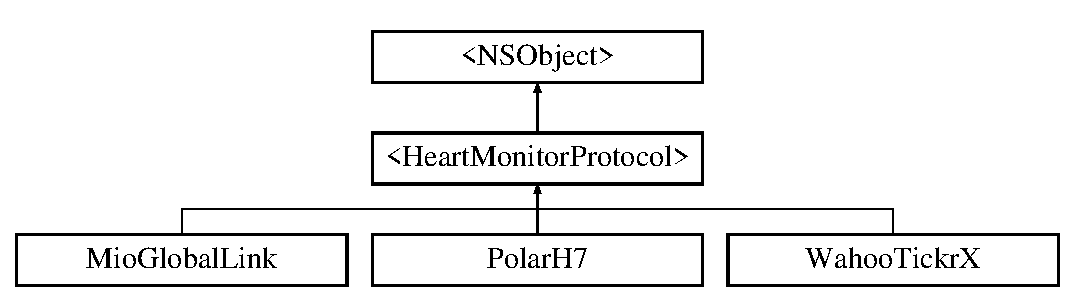
\includegraphics[height=3.000000cm]{protocol_heart_monitor_protocol-p}
\end{center}
\end{figure}
\subsection*{Instance Methods}
\begin{DoxyCompactItemize}
\item 
(N\-S\-Integer) -\/ \hyperlink{protocol_heart_monitor_protocol-p_aa72bff46636870665bae0ab500eb19c1}{get\-Heart\-Rate}
\end{DoxyCompactItemize}


\subsection{Detailed Description}
This protocol is designed to be used on all heart rate monitor devices. The methods enclosed ensure uniform operation with the application, irrespective of the specific device. It is used for polling so that all modifications are to the specific device and do not have cascading effects to the other devices. 

\subsection{Method Documentation}
\hypertarget{protocol_heart_monitor_protocol-p_aa72bff46636870665bae0ab500eb19c1}{\index{Heart\-Monitor\-Protocol-\/p@{Heart\-Monitor\-Protocol-\/p}!get\-Heart\-Rate@{get\-Heart\-Rate}}
\index{get\-Heart\-Rate@{get\-Heart\-Rate}!HeartMonitorProtocol-p@{Heart\-Monitor\-Protocol-\/p}}
\subsubsection[{get\-Heart\-Rate}]{\setlength{\rightskip}{0pt plus 5cm}-\/ (N\-S\-Integer) get\-Heart\-Rate 
\begin{DoxyParamCaption}
{}
\end{DoxyParamCaption}
}}\label{protocol_heart_monitor_protocol-p_aa72bff46636870665bae0ab500eb19c1}
This method gets the current heart rate value from the monitor that utilizes this protocol.

\begin{DoxyReturn}{Returns}
An integer of the currently record heart rate from the heart rate monitor. 
\end{DoxyReturn}


The documentation for this protocol was generated from the following file\-:\begin{DoxyCompactItemize}
\item 
/\-Users/douglas/\-Documents/software/\-Senior Project/ios/\-Medical Cyborgs/\-Medical Cyborgs/Heart\-Monitor\-Protocol.\-h\end{DoxyCompactItemize}

\hypertarget{interface_heart_monitor_select_v_c}{\section{Heart\-Monitor\-Select\-V\-C Class Reference}
\label{interface_heart_monitor_select_v_c}\index{Heart\-Monitor\-Select\-V\-C@{Heart\-Monitor\-Select\-V\-C}}
}


{\ttfamily \#import $<$Heart\-Monitor\-Select\-V\-C.\-h$>$}

Inheritance diagram for Heart\-Monitor\-Select\-V\-C\-:\begin{figure}[H]
\begin{center}
\leavevmode
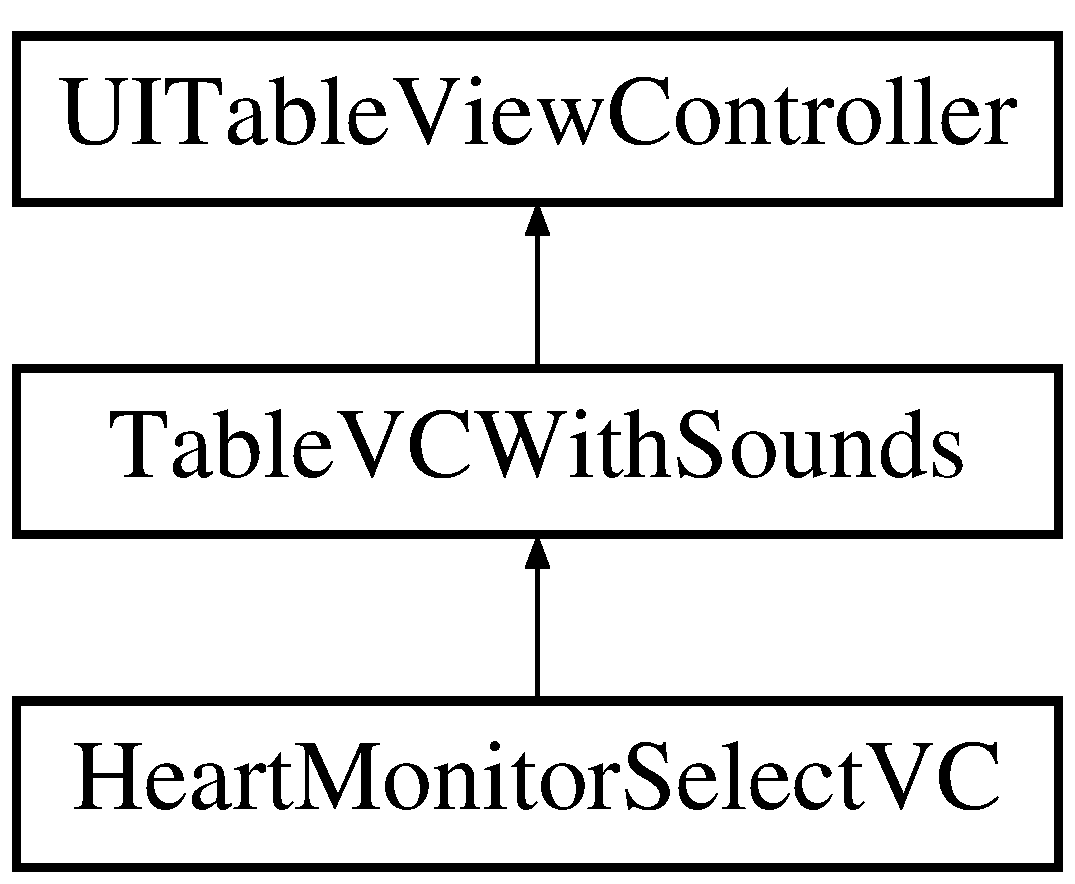
\includegraphics[height=3.000000cm]{interface_heart_monitor_select_v_c}
\end{center}
\end{figure}
\subsection*{Additional Inherited Members}


\subsection{Detailed Description}
This screen does the device selection for devices that have been discovered that perform heart monitoring functions. 

The documentation for this class was generated from the following file\-:\begin{DoxyCompactItemize}
\item 
Heart\-Monitor\-Select\-V\-C.\-h\end{DoxyCompactItemize}

\hypertarget{category_heart_monitor_select_v_c_07_08}{\section{Heart\-Monitor\-Select\-V\-C() Category Reference}
\label{category_heart_monitor_select_v_c_07_08}\index{Heart\-Monitor\-Select\-V\-C()@{Heart\-Monitor\-Select\-V\-C()}}
}


The documentation for this category was generated from the following file\-:\begin{DoxyCompactItemize}
\item 
Heart\-Monitor\-Select\-V\-C.\-m\end{DoxyCompactItemize}

\hypertarget{interface_home_screen_v_c}{\section{Home\-Screen\-V\-C Class Reference}
\label{interface_home_screen_v_c}\index{Home\-Screen\-V\-C@{Home\-Screen\-V\-C}}
}


{\ttfamily \#import $<$Home\-Screen\-V\-C.\-h$>$}

Inheritance diagram for Home\-Screen\-V\-C\-:\begin{figure}[H]
\begin{center}
\leavevmode
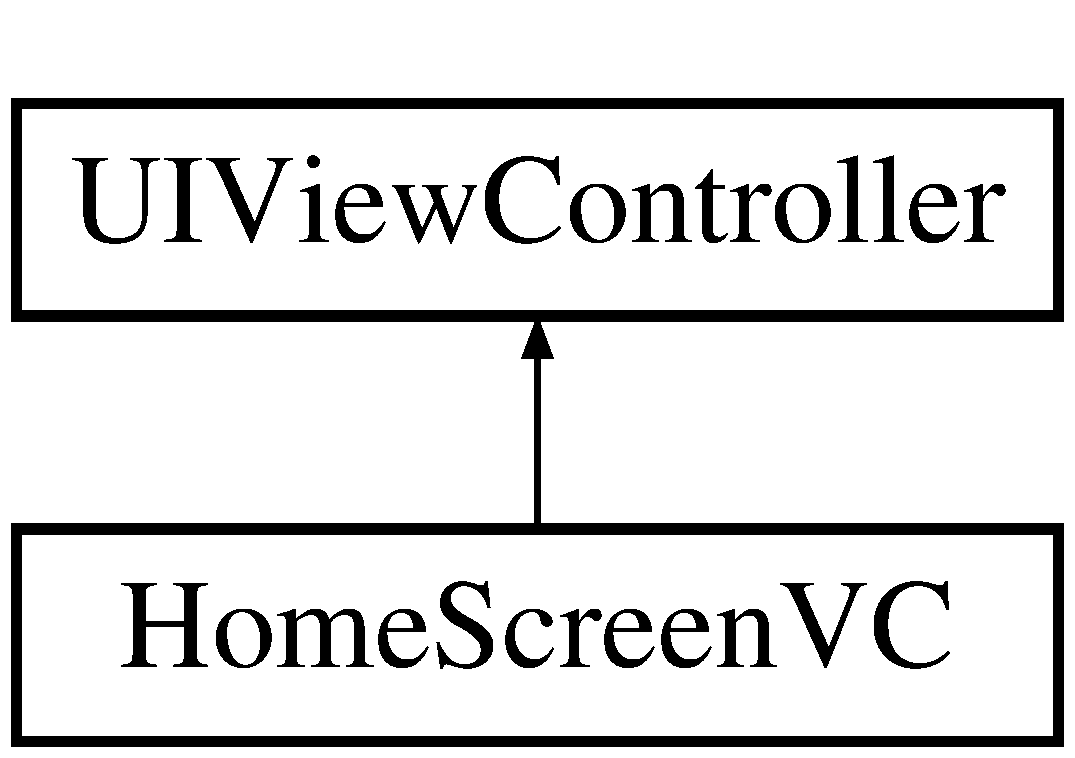
\includegraphics[height=2.000000cm]{interface_home_screen_v_c}
\end{center}
\end{figure}
\subsection*{Instance Methods}
\begin{DoxyCompactItemize}
\item 
\hypertarget{interface_home_screen_v_c_aba4765dac13e0c3829c52a23d6c6b773}{(id) -\/ {\bfseries init\-With\-Background\-Scheduler\-:}}\label{interface_home_screen_v_c_aba4765dac13e0c3829c52a23d6c6b773}

\item 
(I\-B\-Action) -\/ \hyperlink{interface_home_screen_v_c_a8a98314cf71cd518e63b9ce589b35f02}{alter\-Personal\-Settings\-:}
\item 
(I\-B\-Action) -\/ \hyperlink{interface_home_screen_v_c_a3b9db379f6432201f499008c3918fa5f}{select\-Activity\-Monitor\-:}
\item 
(I\-B\-Action) -\/ \hyperlink{interface_home_screen_v_c_a9cf7d44e5fa97a7f70e116ba0b4c6b2c}{select\-Heart\-Monitor\-:}
\item 
(void) -\/ \hyperlink{interface_home_screen_v_c_ac0077075c9e48561794e5e6818232bd9}{set\-Color\-For\-Button\-:is\-Ready\-:}
\item 
(I\-B\-Action) -\/ \hyperlink{interface_home_screen_v_c_a50a2ea69f594741ce8926b4a8f6382f0}{show\-Graph\-:}
\item 
(I\-B\-Action) -\/ \hyperlink{interface_home_screen_v_c_a7cda2112b655ee8a7b622fbfa2ea0d0f}{toggle\-Monitoring\-:}
\item 
(void) -\/ \hyperlink{interface_home_screen_v_c_a83dbe8e2e8729282f47e1ffaf30b07f4}{check\-For\-Updated\-Patient\-I\-D}
\item 
(void) -\/ \hyperlink{interface_home_screen_v_c_a379c482616bb7911c6e9fc71cf9eb2a0}{poll\-Failed\-:}
\end{DoxyCompactItemize}
\subsection*{Properties}
\begin{DoxyCompactItemize}
\item 
\hypertarget{interface_home_screen_v_c_af710ad88b755f5ac91d32478a385af6f}{I\-B\-Outlet U\-I\-Button $\ast$ {\bfseries heart\-Rate\-Button}}\label{interface_home_screen_v_c_af710ad88b755f5ac91d32478a385af6f}

\item 
\hypertarget{interface_home_screen_v_c_aaf7bc9fa4c07923d2df10b9dc6977c02}{I\-B\-Outlet U\-I\-Button $\ast$ {\bfseries activity\-Button}}\label{interface_home_screen_v_c_aaf7bc9fa4c07923d2df10b9dc6977c02}

\item 
\hypertarget{interface_home_screen_v_c_a1e29323a37c594f0e641d1f660605721}{I\-B\-Outlet U\-I\-Button $\ast$ {\bfseries graph\-Button}}\label{interface_home_screen_v_c_a1e29323a37c594f0e641d1f660605721}

\item 
\hypertarget{interface_home_screen_v_c_aad6f8311d7f241d28c255af76fea1c4b}{I\-B\-Outlet U\-I\-Button $\ast$ {\bfseries toggle\-Run\-Button}}\label{interface_home_screen_v_c_aad6f8311d7f241d28c255af76fea1c4b}

\item 
\hypertarget{interface_home_screen_v_c_a8324fe604c4a1dae3d45f9b6fb63d80f}{I\-B\-Outlet U\-I\-Button $\ast$ {\bfseries personal\-Info\-Button}}\label{interface_home_screen_v_c_a8324fe604c4a1dae3d45f9b6fb63d80f}

\item 
\hypertarget{interface_home_screen_v_c_afa80d36d3ba21b19c0aea885cc76f811}{B\-O\-O\-L {\bfseries is\-Monitoring}}\label{interface_home_screen_v_c_afa80d36d3ba21b19c0aea885cc76f811}

\item 
\hypertarget{interface_home_screen_v_c_a89f03faa7fe6fba12a8d17dead120a0c}{\hyperlink{interface_patient_information_v_c}{Patient\-Information\-V\-C} $\ast$ {\bfseries settings}}\label{interface_home_screen_v_c_a89f03faa7fe6fba12a8d17dead120a0c}

\item 
\hypertarget{interface_home_screen_v_c_a2d29b010a455bf37937421fac3bfde81}{\hyperlink{interface_b_t_device_manager}{B\-T\-Device\-Manager} $\ast$ {\bfseries bt\-Devices}}\label{interface_home_screen_v_c_a2d29b010a455bf37937421fac3bfde81}

\item 
\hypertarget{interface_home_screen_v_c_a18a3276c68060f2a0fdd9fbfd32416ab}{\hyperlink{interface_personal_info}{Personal\-Info} $\ast$ {\bfseries patient\-Info}}\label{interface_home_screen_v_c_a18a3276c68060f2a0fdd9fbfd32416ab}

\item 
\hypertarget{interface_home_screen_v_c_a2a965b7384a780e031c9cb85d18aeeb1}{\hyperlink{interface_device_poll_manager}{Device\-Poll\-Manager} $\ast$ {\bfseries device\-Poller}}\label{interface_home_screen_v_c_a2a965b7384a780e031c9cb85d18aeeb1}

\item 
\hypertarget{interface_home_screen_v_c_acf743bf5899a89cff1321f785b9a48e5}{\hyperlink{interface_remote_d_b_connection_manager}{Remote\-D\-B\-Connection\-Manager} $\ast$ {\bfseries server\-Poller}}\label{interface_home_screen_v_c_acf743bf5899a89cff1321f785b9a48e5}

\item 
\hypertarget{interface_home_screen_v_c_a9b110975a1b591e149fc83c768312673}{\hyperlink{interface_background_scheduler}{Background\-Scheduler} $\ast$ {\bfseries scheduler}}\label{interface_home_screen_v_c_a9b110975a1b591e149fc83c768312673}

\end{DoxyCompactItemize}


\subsection{Detailed Description}
This is the first screen you see when the application starts. It provides buttons to navigate through device selection, patient information setup and toggle the monitoring for the application. 

\subsection{Method Documentation}
\hypertarget{interface_home_screen_v_c_a8a98314cf71cd518e63b9ce589b35f02}{\index{Home\-Screen\-V\-C@{Home\-Screen\-V\-C}!alter\-Personal\-Settings\-:@{alter\-Personal\-Settings\-:}}
\index{alter\-Personal\-Settings\-:@{alter\-Personal\-Settings\-:}!HomeScreenVC@{Home\-Screen\-V\-C}}
\subsubsection[{alter\-Personal\-Settings\-:}]{\setlength{\rightskip}{0pt plus 5cm}-\/ (I\-B\-Action) alter\-Personal\-Settings\-: 
\begin{DoxyParamCaption}
\item[{(id)}]{sender}
\end{DoxyParamCaption}
}}\label{interface_home_screen_v_c_a8a98314cf71cd518e63b9ce589b35f02}
This method sets up the U\-I\-View\-Controller to display the personal settings page. It is a standard I\-B\-Action style of method with the signature of (id) sender and a void return value noted as I\-B\-Action for use in the interface builder.


\begin{DoxyParams}{Parameters}
{\em sender} & is not used. \\
\hline
\end{DoxyParams}
\hypertarget{interface_home_screen_v_c_a83dbe8e2e8729282f47e1ffaf30b07f4}{\index{Home\-Screen\-V\-C@{Home\-Screen\-V\-C}!check\-For\-Updated\-Patient\-I\-D@{check\-For\-Updated\-Patient\-I\-D}}
\index{check\-For\-Updated\-Patient\-I\-D@{check\-For\-Updated\-Patient\-I\-D}!HomeScreenVC@{Home\-Screen\-V\-C}}
\subsubsection[{check\-For\-Updated\-Patient\-I\-D}]{\setlength{\rightskip}{0pt plus 5cm}-\/ (void) check\-For\-Updated\-Patient\-I\-D 
\begin{DoxyParamCaption}
{}
\end{DoxyParamCaption}
}}\label{interface_home_screen_v_c_a83dbe8e2e8729282f47e1ffaf30b07f4}
This method checks to see if the patient\-I\-D has been updated. It is used because of the network delay and the delay for the userdefaults on synchronization. \hypertarget{interface_home_screen_v_c_a379c482616bb7911c6e9fc71cf9eb2a0}{\index{Home\-Screen\-V\-C@{Home\-Screen\-V\-C}!poll\-Failed\-:@{poll\-Failed\-:}}
\index{poll\-Failed\-:@{poll\-Failed\-:}!HomeScreenVC@{Home\-Screen\-V\-C}}
\subsubsection[{poll\-Failed\-:}]{\setlength{\rightskip}{0pt plus 5cm}-\/ (void) poll\-Failed\-: 
\begin{DoxyParamCaption}
\item[{(N\-S\-Notification$\ast$)}]{notification}
\end{DoxyParamCaption}
}}\label{interface_home_screen_v_c_a379c482616bb7911c6e9fc71cf9eb2a0}
This method is called when a notification is given by the device poller. It determines how the U\-I is to respond to the event. \hypertarget{interface_home_screen_v_c_a3b9db379f6432201f499008c3918fa5f}{\index{Home\-Screen\-V\-C@{Home\-Screen\-V\-C}!select\-Activity\-Monitor\-:@{select\-Activity\-Monitor\-:}}
\index{select\-Activity\-Monitor\-:@{select\-Activity\-Monitor\-:}!HomeScreenVC@{Home\-Screen\-V\-C}}
\subsubsection[{select\-Activity\-Monitor\-:}]{\setlength{\rightskip}{0pt plus 5cm}-\/ (I\-B\-Action) select\-Activity\-Monitor\-: 
\begin{DoxyParamCaption}
\item[{(id)}]{sender}
\end{DoxyParamCaption}
}}\label{interface_home_screen_v_c_a3b9db379f6432201f499008c3918fa5f}
This method sets up the U\-I\-View\-Controller to display the activity monitor selection page. It is a standard I\-B\-Action style of method with the signature of (id) sender and a void return value noted as I\-B\-Action for use in the interface builder.


\begin{DoxyParams}{Parameters}
{\em sender} & is not used. \\
\hline
\end{DoxyParams}
\hypertarget{interface_home_screen_v_c_a9cf7d44e5fa97a7f70e116ba0b4c6b2c}{\index{Home\-Screen\-V\-C@{Home\-Screen\-V\-C}!select\-Heart\-Monitor\-:@{select\-Heart\-Monitor\-:}}
\index{select\-Heart\-Monitor\-:@{select\-Heart\-Monitor\-:}!HomeScreenVC@{Home\-Screen\-V\-C}}
\subsubsection[{select\-Heart\-Monitor\-:}]{\setlength{\rightskip}{0pt plus 5cm}-\/ (I\-B\-Action) select\-Heart\-Monitor\-: 
\begin{DoxyParamCaption}
\item[{(id)}]{sender}
\end{DoxyParamCaption}
}}\label{interface_home_screen_v_c_a9cf7d44e5fa97a7f70e116ba0b4c6b2c}
This method sets up the U\-I\-View\-Controller to display the heart monitor selection page. It is a standard I\-B\-Action style of method with the signature of (id) sender and a void return value noted as I\-B\-Action for use in the interface builder.


\begin{DoxyParams}{Parameters}
{\em sender} & is not used. \\
\hline
\end{DoxyParams}
\hypertarget{interface_home_screen_v_c_ac0077075c9e48561794e5e6818232bd9}{\index{Home\-Screen\-V\-C@{Home\-Screen\-V\-C}!set\-Color\-For\-Button\-:is\-Ready\-:@{set\-Color\-For\-Button\-:is\-Ready\-:}}
\index{set\-Color\-For\-Button\-:is\-Ready\-:@{set\-Color\-For\-Button\-:is\-Ready\-:}!HomeScreenVC@{Home\-Screen\-V\-C}}
\subsubsection[{set\-Color\-For\-Button\-:is\-Ready\-:}]{\setlength{\rightskip}{0pt plus 5cm}-\/ (void) set\-Color\-For\-Button\-: 
\begin{DoxyParamCaption}
\item[{(U\-I\-Button$\ast$)}]{button}
\item[{isReady:(B\-O\-O\-L)}]{ready}
\end{DoxyParamCaption}
}}\label{interface_home_screen_v_c_ac0077075c9e48561794e5e6818232bd9}
This method changes the color of the button based on whether that function has been configured for use. If the function is not ready the button will get a red hue, otherwise it will get a green hue.


\begin{DoxyParams}{Parameters}
{\em button} & The U\-I\-Button that will be modified for the color change. If none provided no change takes place. \\
\hline
{\em ready} & The ready state. The default is N\-O. \\
\hline
\end{DoxyParams}
\hypertarget{interface_home_screen_v_c_a50a2ea69f594741ce8926b4a8f6382f0}{\index{Home\-Screen\-V\-C@{Home\-Screen\-V\-C}!show\-Graph\-:@{show\-Graph\-:}}
\index{show\-Graph\-:@{show\-Graph\-:}!HomeScreenVC@{Home\-Screen\-V\-C}}
\subsubsection[{show\-Graph\-:}]{\setlength{\rightskip}{0pt plus 5cm}-\/ (I\-B\-Action) show\-Graph\-: 
\begin{DoxyParamCaption}
\item[{(id)}]{sender}
\end{DoxyParamCaption}
}}\label{interface_home_screen_v_c_a50a2ea69f594741ce8926b4a8f6382f0}
This method sets up the U\-I\-View\-Controller to display the graph page. This page will only display if the other devices are connected. Its purpose is to show real time collection of data. It is a standard I\-B\-Action style of method with the signature of (id) sender and a void return value noted as I\-B\-Action for use in the interface builder.


\begin{DoxyParams}{Parameters}
{\em sender} & is not used. \\
\hline
\end{DoxyParams}
\hypertarget{interface_home_screen_v_c_a7cda2112b655ee8a7b622fbfa2ea0d0f}{\index{Home\-Screen\-V\-C@{Home\-Screen\-V\-C}!toggle\-Monitoring\-:@{toggle\-Monitoring\-:}}
\index{toggle\-Monitoring\-:@{toggle\-Monitoring\-:}!HomeScreenVC@{Home\-Screen\-V\-C}}
\subsubsection[{toggle\-Monitoring\-:}]{\setlength{\rightskip}{0pt plus 5cm}-\/ (I\-B\-Action) toggle\-Monitoring\-: 
\begin{DoxyParamCaption}
\item[{(id)}]{sender}
\end{DoxyParamCaption}
}}\label{interface_home_screen_v_c_a7cda2112b655ee8a7b622fbfa2ea0d0f}
This method starts and stops the actual monitoring process. It does the setup and tear down of the backgroun thread that pulls information from the devices at certain intervals and uploads to the remote database at other intervals. It is a standard I\-B\-Action style of method with the signature of (id) sender and a void return value noted as I\-B\-Action for use in the interface builder.


\begin{DoxyParams}{Parameters}
{\em sender} & is not used. \\
\hline
\end{DoxyParams}


The documentation for this class was generated from the following files\-:\begin{DoxyCompactItemize}
\item 
Home\-Screen\-V\-C.\-h\item 
Home\-Screen\-V\-C.\-m\end{DoxyCompactItemize}

\hypertarget{category_home_screen_v_c_07_08}{\section{Home\-Screen\-V\-C() Category Reference}
\label{category_home_screen_v_c_07_08}\index{Home\-Screen\-V\-C()@{Home\-Screen\-V\-C()}}
}


The documentation for this category was generated from the following file\-:\begin{DoxyCompactItemize}
\item 
Home\-Screen\-V\-C.\-m\end{DoxyCompactItemize}

\hypertarget{interface_jawbone_u_p24}{\section{Jawbone\-U\-P24 Class Reference}
\label{interface_jawbone_u_p24}\index{Jawbone\-U\-P24@{Jawbone\-U\-P24}}
}
Inheritance diagram for Jawbone\-U\-P24\-:\begin{figure}[H]
\begin{center}
\leavevmode
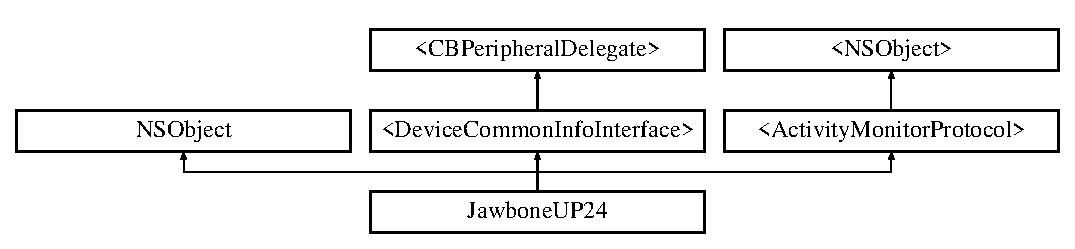
\includegraphics[height=2.901554cm]{interface_jawbone_u_p24}
\end{center}
\end{figure}
\subsection*{Properties}
\begin{DoxyCompactItemize}
\item 
N\-S\-Integer \hyperlink{interface_jawbone_u_p24_abd2f3cf19e5f5feeef6be3cf2193acce}{type}
\item 
C\-B\-Service $\ast$ \hyperlink{interface_jawbone_u_p24_a60f0270de3139d5219544969cce08293}{battery\-Service}
\item 
C\-B\-Characteristic $\ast$ \hyperlink{interface_jawbone_u_p24_ac0feafa5d2a26db099b3328df1cc85e1}{battery\-Lvl\-Char}
\item 
int \hyperlink{interface_jawbone_u_p24_a7c1af9ec44bfb9a3fafcf6d3ba1a3dc9}{battery\-Level}
\item 
C\-B\-Peripheral $\ast$ \hyperlink{interface_jawbone_u_p24_a9ed19c4b26f90dfbf9523ba2b7dbf6e0}{device}
\item 
N\-S\-String $\ast$ \hyperlink{interface_jawbone_u_p24_af3f464123aa078ff318eecfba7bbcaf4}{device\-Manufacturer}
\end{DoxyCompactItemize}
\subsection*{Additional Inherited Members}


\subsection{Property Documentation}
\hypertarget{interface_jawbone_u_p24_a7c1af9ec44bfb9a3fafcf6d3ba1a3dc9}{\index{Jawbone\-U\-P24@{Jawbone\-U\-P24}!battery\-Level@{battery\-Level}}
\index{battery\-Level@{battery\-Level}!JawboneUP24@{Jawbone\-U\-P24}}
\subsubsection[{battery\-Level}]{\setlength{\rightskip}{0pt plus 5cm}-\/ (int) battery\-Level\hspace{0.3cm}{\ttfamily [read]}, {\ttfamily [write]}, {\ttfamily [atomic]}}}\label{interface_jawbone_u_p24_a7c1af9ec44bfb9a3fafcf6d3ba1a3dc9}
The last known integer value of the battery percentage. The default is 0 if the battery level is not read. \hypertarget{interface_jawbone_u_p24_ac0feafa5d2a26db099b3328df1cc85e1}{\index{Jawbone\-U\-P24@{Jawbone\-U\-P24}!battery\-Lvl\-Char@{battery\-Lvl\-Char}}
\index{battery\-Lvl\-Char@{battery\-Lvl\-Char}!JawboneUP24@{Jawbone\-U\-P24}}
\subsubsection[{battery\-Lvl\-Char}]{\setlength{\rightskip}{0pt plus 5cm}-\/ (C\-B\-Characteristic$\ast$) battery\-Lvl\-Char\hspace{0.3cm}{\ttfamily [read]}, {\ttfamily [write]}, {\ttfamily [atomic]}, {\ttfamily [retain]}}}\label{interface_jawbone_u_p24_ac0feafa5d2a26db099b3328df1cc85e1}
The C\-B\-Characteristic reference for use in reading the battery level of the device. \hypertarget{interface_jawbone_u_p24_a60f0270de3139d5219544969cce08293}{\index{Jawbone\-U\-P24@{Jawbone\-U\-P24}!battery\-Service@{battery\-Service}}
\index{battery\-Service@{battery\-Service}!JawboneUP24@{Jawbone\-U\-P24}}
\subsubsection[{battery\-Service}]{\setlength{\rightskip}{0pt plus 5cm}-\/ (C\-B\-Service$\ast$) battery\-Service\hspace{0.3cm}{\ttfamily [read]}, {\ttfamily [write]}, {\ttfamily [atomic]}, {\ttfamily [retain]}}}\label{interface_jawbone_u_p24_a60f0270de3139d5219544969cce08293}
The C\-B\-Service reference for use in detecting the battery level of the device. \hypertarget{interface_jawbone_u_p24_a9ed19c4b26f90dfbf9523ba2b7dbf6e0}{\index{Jawbone\-U\-P24@{Jawbone\-U\-P24}!device@{device}}
\index{device@{device}!JawboneUP24@{Jawbone\-U\-P24}}
\subsubsection[{device}]{\setlength{\rightskip}{0pt plus 5cm}-\/ (C\-B\-Peripheral$\ast$) device\hspace{0.3cm}{\ttfamily [read]}, {\ttfamily [write]}, {\ttfamily [atomic]}, {\ttfamily [retain]}}}\label{interface_jawbone_u_p24_a9ed19c4b26f90dfbf9523ba2b7dbf6e0}
The C\-B\-Peripheral device that was discovered and used with this class. \hypertarget{interface_jawbone_u_p24_af3f464123aa078ff318eecfba7bbcaf4}{\index{Jawbone\-U\-P24@{Jawbone\-U\-P24}!device\-Manufacturer@{device\-Manufacturer}}
\index{device\-Manufacturer@{device\-Manufacturer}!JawboneUP24@{Jawbone\-U\-P24}}
\subsubsection[{device\-Manufacturer}]{\setlength{\rightskip}{0pt plus 5cm}-\/ (N\-S\-String$\ast$) device\-Manufacturer\hspace{0.3cm}{\ttfamily [read]}, {\ttfamily [write]}, {\ttfamily [atomic]}, {\ttfamily [retain]}}}\label{interface_jawbone_u_p24_af3f464123aa078ff318eecfba7bbcaf4}
The N\-S\-String value of the manufacturer as read from the device. \hypertarget{interface_jawbone_u_p24_abd2f3cf19e5f5feeef6be3cf2193acce}{\index{Jawbone\-U\-P24@{Jawbone\-U\-P24}!type@{type}}
\index{type@{type}!JawboneUP24@{Jawbone\-U\-P24}}
\subsubsection[{type}]{\setlength{\rightskip}{0pt plus 5cm}-\/ (N\-S\-Integer) type\hspace{0.3cm}{\ttfamily [read]}, {\ttfamily [write]}, {\ttfamily [atomic]}}}\label{interface_jawbone_u_p24_abd2f3cf19e5f5feeef6be3cf2193acce}
The device type as an enum of Device\-Type. See \hyperlink{_device_types_8h_source}{Device\-Types.\-h} for details. 

The documentation for this class was generated from the following files\-:\begin{DoxyCompactItemize}
\item 
/\-Users/douglas/\-Documents/software/\-Senior Project/ios/\-Medical Cyborgs/\-Medical Cyborgs/Jawbone\-U\-P24.\-h\item 
/\-Users/douglas/\-Documents/software/\-Senior Project/ios/\-Medical Cyborgs/\-Medical Cyborgs/Jawbone\-U\-P24.\-m\end{DoxyCompactItemize}

\hypertarget{interface_local_d_b_result}{\section{Local\-D\-B\-Result Class Reference}
\label{interface_local_d_b_result}\index{Local\-D\-B\-Result@{Local\-D\-B\-Result}}
}


{\ttfamily \#import $<$Local\-D\-B\-Result.\-h$>$}

Inheritance diagram for Local\-D\-B\-Result\-:\begin{figure}[H]
\begin{center}
\leavevmode
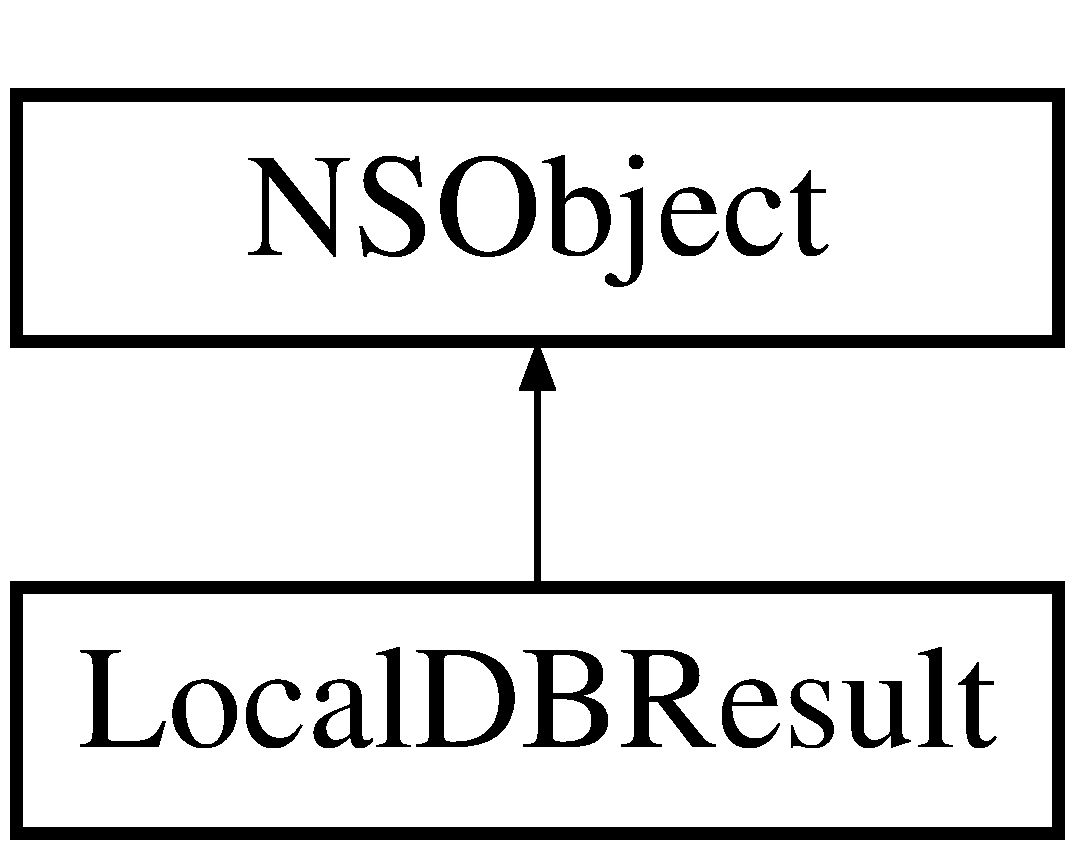
\includegraphics[height=2.000000cm]{interface_local_d_b_result}
\end{center}
\end{figure}
\subsection*{Properties}
\begin{DoxyCompactItemize}
\item 
N\-S\-Integer \hyperlink{interface_local_d_b_result_a5cdd651e87ce4b0e2ed296fd1a54f271}{patient\-I\-D}
\item 
N\-S\-Integer \hyperlink{interface_local_d_b_result_a59bb8d9536b92e3bbd6c244d13771ccc}{heart\-Rate}
\item 
float \hyperlink{interface_local_d_b_result_a55f83e49659fb4d15db30117f90dcea7}{latitude}
\item 
float \hyperlink{interface_local_d_b_result_ae50e0676b6cac4cad3e565c5caa117b2}{longitude}
\item 
N\-S\-String $\ast$ \hyperlink{interface_local_d_b_result_a7538fcbcfd150e5353d3d4e531bef2bc}{time\-Stamp}
\item 
N\-S\-Integer \hyperlink{interface_local_d_b_result_a10d275e102bd14b0a071b5572fbf62d3}{activity\-Level}
\end{DoxyCompactItemize}


\subsection{Detailed Description}
This is a simple data class that is used to pass around from the database to classes that are using it. It was created to simplify string manipulation. 

\subsection{Property Documentation}
\hypertarget{interface_local_d_b_result_a10d275e102bd14b0a071b5572fbf62d3}{\index{Local\-D\-B\-Result@{Local\-D\-B\-Result}!activity\-Level@{activity\-Level}}
\index{activity\-Level@{activity\-Level}!LocalDBResult@{Local\-D\-B\-Result}}
\subsubsection[{activity\-Level}]{\setlength{\rightskip}{0pt plus 5cm}-\/ (N\-S\-Integer) activity\-Level\hspace{0.3cm}{\ttfamily [read]}, {\ttfamily [write]}, {\ttfamily [atomic]}}}\label{interface_local_d_b_result_a10d275e102bd14b0a071b5572fbf62d3}
An integer value of the activity level based on patient age and heart rate. See \hyperlink{class_device_constants_and_static_functions}{Device\-Constants\-And\-Static\-Functions} for a description. \hypertarget{interface_local_d_b_result_a59bb8d9536b92e3bbd6c244d13771ccc}{\index{Local\-D\-B\-Result@{Local\-D\-B\-Result}!heart\-Rate@{heart\-Rate}}
\index{heart\-Rate@{heart\-Rate}!LocalDBResult@{Local\-D\-B\-Result}}
\subsubsection[{heart\-Rate}]{\setlength{\rightskip}{0pt plus 5cm}-\/ (N\-S\-Integer) heart\-Rate\hspace{0.3cm}{\ttfamily [read]}, {\ttfamily [write]}, {\ttfamily [atomic]}}}\label{interface_local_d_b_result_a59bb8d9536b92e3bbd6c244d13771ccc}
The heart rate of the patient as it was recorded by the database. \hypertarget{interface_local_d_b_result_a55f83e49659fb4d15db30117f90dcea7}{\index{Local\-D\-B\-Result@{Local\-D\-B\-Result}!latitude@{latitude}}
\index{latitude@{latitude}!LocalDBResult@{Local\-D\-B\-Result}}
\subsubsection[{latitude}]{\setlength{\rightskip}{0pt plus 5cm}-\/ (float) latitude\hspace{0.3cm}{\ttfamily [read]}, {\ttfamily [write]}, {\ttfamily [atomic]}}}\label{interface_local_d_b_result_a55f83e49659fb4d15db30117f90dcea7}
The latitude of the patient that was recorded. This value will not change much unless big changes happen. \hypertarget{interface_local_d_b_result_ae50e0676b6cac4cad3e565c5caa117b2}{\index{Local\-D\-B\-Result@{Local\-D\-B\-Result}!longitude@{longitude}}
\index{longitude@{longitude}!LocalDBResult@{Local\-D\-B\-Result}}
\subsubsection[{longitude}]{\setlength{\rightskip}{0pt plus 5cm}-\/ (float) longitude\hspace{0.3cm}{\ttfamily [read]}, {\ttfamily [write]}, {\ttfamily [atomic]}}}\label{interface_local_d_b_result_ae50e0676b6cac4cad3e565c5caa117b2}
The longitude of the patient that was recorded. This value will not change much unless big changes happen. \hypertarget{interface_local_d_b_result_a5cdd651e87ce4b0e2ed296fd1a54f271}{\index{Local\-D\-B\-Result@{Local\-D\-B\-Result}!patient\-I\-D@{patient\-I\-D}}
\index{patient\-I\-D@{patient\-I\-D}!LocalDBResult@{Local\-D\-B\-Result}}
\subsubsection[{patient\-I\-D}]{\setlength{\rightskip}{0pt plus 5cm}-\/ (N\-S\-Integer) patient\-I\-D\hspace{0.3cm}{\ttfamily [read]}, {\ttfamily [write]}, {\ttfamily [atomic]}}}\label{interface_local_d_b_result_a5cdd651e87ce4b0e2ed296fd1a54f271}
The patient\-I\-D that is used by the database. \hypertarget{interface_local_d_b_result_a7538fcbcfd150e5353d3d4e531bef2bc}{\index{Local\-D\-B\-Result@{Local\-D\-B\-Result}!time\-Stamp@{time\-Stamp}}
\index{time\-Stamp@{time\-Stamp}!LocalDBResult@{Local\-D\-B\-Result}}
\subsubsection[{time\-Stamp}]{\setlength{\rightskip}{0pt plus 5cm}-\/ (N\-S\-String$\ast$) time\-Stamp\hspace{0.3cm}{\ttfamily [read]}, {\ttfamily [write]}, {\ttfamily [atomic]}}}\label{interface_local_d_b_result_a7538fcbcfd150e5353d3d4e531bef2bc}
The timestamp this data was recorded in the database. It has date and time. It follows the format of 'yyyy-\/mm-\/dd hh\-:mm\-:ss'. The hours are expressed in military time from 0-\/23. 

The documentation for this class was generated from the following file\-:\begin{DoxyCompactItemize}
\item 
/\-Users/douglas/\-Documents/software/\-Senior Project/ios/\-Medical Cyborgs/\-Medical Cyborgs/Local\-D\-B\-Result.\-h\end{DoxyCompactItemize}

\hypertarget{interface_mio_global_link}{\section{Mio\-Global\-Link Class Reference}
\label{interface_mio_global_link}\index{Mio\-Global\-Link@{Mio\-Global\-Link}}
}
Inheritance diagram for Mio\-Global\-Link\-:\begin{figure}[H]
\begin{center}
\leavevmode
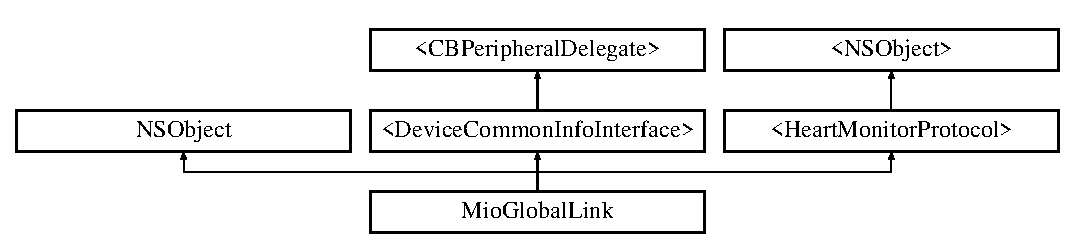
\includegraphics[height=2.901554cm]{interface_mio_global_link}
\end{center}
\end{figure}
\subsection*{Properties}
\begin{DoxyCompactItemize}
\item 
\hypertarget{interface_mio_global_link_a82edb3dd6e24af3fb2ed9061e2c2b21f}{N\-S\-Integer {\bfseries type}}\label{interface_mio_global_link_a82edb3dd6e24af3fb2ed9061e2c2b21f}

\item 
\hypertarget{interface_mio_global_link_a6615e890d11dfb95046f5f229f789f8e}{C\-B\-Service $\ast$ {\bfseries battery\-Service}}\label{interface_mio_global_link_a6615e890d11dfb95046f5f229f789f8e}

\item 
\hypertarget{interface_mio_global_link_a77ed04d9593004c08ec49e1620cd79a0}{C\-B\-Characteristic $\ast$ {\bfseries battery\-Lvl\-Char}}\label{interface_mio_global_link_a77ed04d9593004c08ec49e1620cd79a0}

\item 
\hypertarget{interface_mio_global_link_af59bfad40ad67f8cc419f3242f04500b}{C\-B\-Service $\ast$ {\bfseries heart\-Rate\-Service}}\label{interface_mio_global_link_af59bfad40ad67f8cc419f3242f04500b}

\item 
\hypertarget{interface_mio_global_link_a6d0625aca6d7b1638753cb5e321e9632}{C\-B\-Characteristic $\ast$ {\bfseries heart\-Rate\-Char}}\label{interface_mio_global_link_a6d0625aca6d7b1638753cb5e321e9632}

\item 
\hypertarget{interface_mio_global_link_a7f0add9d273f0d51eb4b3c73f3eb167d}{int {\bfseries battery\-Level}}\label{interface_mio_global_link_a7f0add9d273f0d51eb4b3c73f3eb167d}

\item 
\hypertarget{interface_mio_global_link_a8d4650fecd6a5f86366446e862be7f21}{C\-B\-Peripheral $\ast$ {\bfseries device}}\label{interface_mio_global_link_a8d4650fecd6a5f86366446e862be7f21}

\item 
\hypertarget{interface_mio_global_link_a5d67ddaf6d5941b85f93196a95630b9d}{N\-S\-String $\ast$ {\bfseries device\-Manufacturer}}\label{interface_mio_global_link_a5d67ddaf6d5941b85f93196a95630b9d}

\item 
\hypertarget{interface_mio_global_link_acb64fafbafbb75c3e6f2c382841f9f06}{N\-S\-Integer {\bfseries current\-Heart\-Rate}}\label{interface_mio_global_link_acb64fafbafbb75c3e6f2c382841f9f06}

\end{DoxyCompactItemize}
\subsection*{Additional Inherited Members}


The documentation for this class was generated from the following files\-:\begin{DoxyCompactItemize}
\item 
Mio\-Global\-Link.\-h\item 
Mio\-Global\-Link.\-m\end{DoxyCompactItemize}

\hypertarget{interface_monitor_creation_factory}{\section{Monitor\-Creation\-Factory Class Reference}
\label{interface_monitor_creation_factory}\index{Monitor\-Creation\-Factory@{Monitor\-Creation\-Factory}}
}


{\ttfamily \#import $<$Monitor\-Creation\-Factory.\-h$>$}

Inheritance diagram for Monitor\-Creation\-Factory\-:\begin{figure}[H]
\begin{center}
\leavevmode
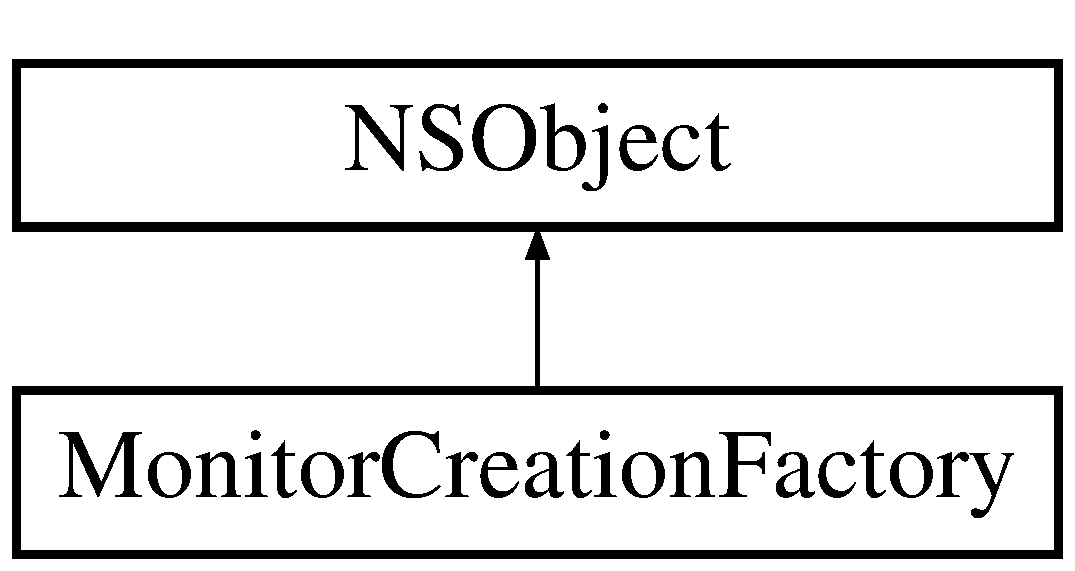
\includegraphics[height=2.000000cm]{interface_monitor_creation_factory}
\end{center}
\end{figure}
\subsection*{Class Methods}
\begin{DoxyCompactItemize}
\item 
(id$<$ \hyperlink{protocol_device_common_info_interface-p}{Device\-Common\-Info\-Interface} $>$) + \hyperlink{interface_monitor_creation_factory_abe947f8b7d9f30a4438112bbdea8dda1}{create\-From\-Peripheral\-:}
\end{DoxyCompactItemize}


\subsection{Detailed Description}
This class is a factory. The purpose is to use polymorphic behavior in the creation of the device classes without the calling class having to know the details. The setup details are in the create\-From\-Peripheral method.

N\-O\-T\-E\-: In order to add more devices to this application the following must be done.


\begin{DoxyEnumerate}
\item A class for that device must be created.
\item The class must at a minimum follow and implement the methods in the \hyperlink{protocol_device_common_info_interface-p}{Device\-Common\-Info\-Interface} protocol.
\item If the device does heart monitoring it must use the methods in the \hyperlink{protocol_heart_monitor_protocol-p}{Heart\-Monitor\-Protocol}.
\item If the device does activity monitoring it must use the methods in the \hyperlink{protocol_activity_monitor_protocol-p}{Activity\-Monitor\-Protocol}.
\item The +(id$<$\-Device\-Common\-Info\-Interface$>$) create\-From\-Peripheral\-: (C\-B\-Peripheral$\ast$) peripheral must be updated
\end{DoxyEnumerate}

This class is a device object factory to centralize creation and reduce dependency complexities as much as possible. 

\subsection{Method Documentation}
\hypertarget{interface_monitor_creation_factory_abe947f8b7d9f30a4438112bbdea8dda1}{\index{Monitor\-Creation\-Factory@{Monitor\-Creation\-Factory}!create\-From\-Peripheral\-:@{create\-From\-Peripheral\-:}}
\index{create\-From\-Peripheral\-:@{create\-From\-Peripheral\-:}!MonitorCreationFactory@{Monitor\-Creation\-Factory}}
\subsubsection[{create\-From\-Peripheral\-:}]{\setlength{\rightskip}{0pt plus 5cm}+ (id$<$ {\bf Device\-Common\-Info\-Interface} $>$) create\-From\-Peripheral\-: 
\begin{DoxyParamCaption}
\item[{(C\-B\-Peripheral$\ast$)}]{peripheral}
\end{DoxyParamCaption}
}}\label{interface_monitor_creation_factory_abe947f8b7d9f30a4438112bbdea8dda1}
Creates a device object based on the peripheral supplied. There are a few assumptions. The first assumption is that there is a class for the type of device to be created. The second assumption is that this method properly identifies the type of device that fits the class and finally that the class is in the import section above this comment. This method does N\-O\-T always produce an object and so a check to see if the return is nil is needed. This is to prevent the false positives sometimes created from the scanning process.


\begin{DoxyParams}{Parameters}
{\em peripheral} & is the device bluetooth device peripheral object that is passed from the device manager. \\
\hline
\end{DoxyParams}
\begin{DoxyReturn}{Returns}
The return is an object of the class that fits in the \hyperlink{protocol_device_common_info_interface-p}{Device\-Common\-Info\-Interface} protocol. All devices must follow the protocol for proper utilization and to prevent runtime crashes. The return value must be checked for nil cases. 
\end{DoxyReturn}


The documentation for this class was generated from the following files\-:\begin{DoxyCompactItemize}
\item 
/\-Users/douglas/\-Documents/software/\-Senior Project/ios/\-Medical Cyborgs/\-Medical Cyborgs/Monitor\-Creation\-Factory.\-h\item 
/\-Users/douglas/\-Documents/software/\-Senior Project/ios/\-Medical Cyborgs/\-Medical Cyborgs/Monitor\-Creation\-Factory.\-m\end{DoxyCompactItemize}

\hypertarget{interface_patient_information_v_c}{\section{Patient\-Information\-V\-C Class Reference}
\label{interface_patient_information_v_c}\index{Patient\-Information\-V\-C@{Patient\-Information\-V\-C}}
}
Inheritance diagram for Patient\-Information\-V\-C\-:\begin{figure}[H]
\begin{center}
\leavevmode
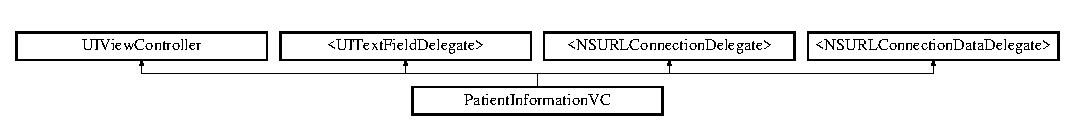
\includegraphics[height=1.308411cm]{interface_patient_information_v_c}
\end{center}
\end{figure}
\subsection*{Instance Methods}
\begin{DoxyCompactItemize}
\item 
(id) -\/ \hyperlink{interface_patient_information_v_c_ab98d9f44b4ee1c4b3051c017ebdac5c5}{init\-With\-Personal\-Information\-:}
\item 
(void) -\/ \hyperlink{interface_patient_information_v_c_ab6fee07f4777f557711e819c9a4cf3a4}{update\-D\-O\-B}
\end{DoxyCompactItemize}
\subsection*{Properties}
\begin{DoxyCompactItemize}
\item 
I\-B\-Outlet U\-I\-Text\-Field $\ast$ \hyperlink{interface_patient_information_v_c_a1836a8d8dc5e1a376109fb8b391c4038}{first\-Name\-Entry}
\item 
I\-B\-Outlet U\-I\-Text\-Field $\ast$ \hyperlink{interface_patient_information_v_c_a6523689959d35fa22fe3e01838ada93c}{last\-Name\-Entry}
\item 
I\-B\-Outlet U\-I\-Date\-Picker $\ast$ \hyperlink{interface_patient_information_v_c_a939dda6df517b4b5a4624928c77fe5b8}{dob\-Selector}
\item 
\hyperlink{interface_personal_info}{Personal\-Info} $\ast$ \hyperlink{interface_patient_information_v_c_afef82a462fd797cc833f72f3b33d9b3c}{patient\-Data}
\item 
N\-S\-Mutable\-Data $\ast$ \hyperlink{interface_patient_information_v_c_a17cd9e90386e04e545017658bf34582e}{\-\_\-server\-Response\-Data}
\end{DoxyCompactItemize}


\subsection{Method Documentation}
\hypertarget{interface_patient_information_v_c_ab98d9f44b4ee1c4b3051c017ebdac5c5}{\index{Patient\-Information\-V\-C@{Patient\-Information\-V\-C}!init\-With\-Personal\-Information\-:@{init\-With\-Personal\-Information\-:}}
\index{init\-With\-Personal\-Information\-:@{init\-With\-Personal\-Information\-:}!PatientInformationVC@{Patient\-Information\-V\-C}}
\subsubsection[{init\-With\-Personal\-Information\-:}]{\setlength{\rightskip}{0pt plus 5cm}-\/ (id) init\-With\-Personal\-Information\-: 
\begin{DoxyParamCaption}
\item[{({\bf Personal\-Info}$\ast$)}]{existing\-Patient\-Data}
\end{DoxyParamCaption}
}}\label{interface_patient_information_v_c_ab98d9f44b4ee1c4b3051c017ebdac5c5}
This method creates a viewcontroller that has the personal information object. The object queries the device store user default settings and maintains the records. This information is needed for building the initial view with patient information.


\begin{DoxyParams}{Parameters}
{\em existing\-Patient\-Data} & is the object that contains the patient name, D\-O\-B, and I\-D necessary for the V\-C to function. \\
\hline
\end{DoxyParams}
\begin{DoxyReturn}{Returns}
A viewcontroller that will display the current patient information and allow editing. 
\end{DoxyReturn}
\hypertarget{interface_patient_information_v_c_ab6fee07f4777f557711e819c9a4cf3a4}{\index{Patient\-Information\-V\-C@{Patient\-Information\-V\-C}!update\-D\-O\-B@{update\-D\-O\-B}}
\index{update\-D\-O\-B@{update\-D\-O\-B}!PatientInformationVC@{Patient\-Information\-V\-C}}
\subsubsection[{update\-D\-O\-B}]{\setlength{\rightskip}{0pt plus 5cm}-\/ (void) update\-D\-O\-B 
\begin{DoxyParamCaption}
{}
\end{DoxyParamCaption}
}}\label{interface_patient_information_v_c_ab6fee07f4777f557711e819c9a4cf3a4}
This method updates the patient information to reflect the date that is selected from the U\-I\-Date\-Picker object. 

\subsection{Property Documentation}
\hypertarget{interface_patient_information_v_c_a17cd9e90386e04e545017658bf34582e}{\index{Patient\-Information\-V\-C@{Patient\-Information\-V\-C}!\-\_\-server\-Response\-Data@{\-\_\-server\-Response\-Data}}
\index{\-\_\-server\-Response\-Data@{\-\_\-server\-Response\-Data}!PatientInformationVC@{Patient\-Information\-V\-C}}
\subsubsection[{\-\_\-server\-Response\-Data}]{\setlength{\rightskip}{0pt plus 5cm}-\/ (N\-S\-Mutable\-Data$\ast$) \-\_\-server\-Response\-Data\hspace{0.3cm}{\ttfamily [read]}, {\ttfamily [write]}, {\ttfamily [atomic]}, {\ttfamily [retain]}}}\label{interface_patient_information_v_c_a17cd9e90386e04e545017658bf34582e}
The data queue used for the network response to build the value of the returned patient I\-D as determined by the remote database. \hypertarget{interface_patient_information_v_c_a939dda6df517b4b5a4624928c77fe5b8}{\index{Patient\-Information\-V\-C@{Patient\-Information\-V\-C}!dob\-Selector@{dob\-Selector}}
\index{dob\-Selector@{dob\-Selector}!PatientInformationVC@{Patient\-Information\-V\-C}}
\subsubsection[{dob\-Selector}]{\setlength{\rightskip}{0pt plus 5cm}-\/ (I\-B\-Outlet U\-I\-Date\-Picker$\ast$) dob\-Selector\hspace{0.3cm}{\ttfamily [read]}, {\ttfamily [write]}, {\ttfamily [nonatomic]}, {\ttfamily [retain]}}}\label{interface_patient_information_v_c_a939dda6df517b4b5a4624928c77fe5b8}
The date picker for selecting the patients date of birth. \hypertarget{interface_patient_information_v_c_a1836a8d8dc5e1a376109fb8b391c4038}{\index{Patient\-Information\-V\-C@{Patient\-Information\-V\-C}!first\-Name\-Entry@{first\-Name\-Entry}}
\index{first\-Name\-Entry@{first\-Name\-Entry}!PatientInformationVC@{Patient\-Information\-V\-C}}
\subsubsection[{first\-Name\-Entry}]{\setlength{\rightskip}{0pt plus 5cm}-\/ (I\-B\-Outlet U\-I\-Text\-Field$\ast$) first\-Name\-Entry\hspace{0.3cm}{\ttfamily [read]}, {\ttfamily [write]}, {\ttfamily [nonatomic]}, {\ttfamily [retain]}}}\label{interface_patient_information_v_c_a1836a8d8dc5e1a376109fb8b391c4038}
The textfield for editing the first name of the patient. \hypertarget{interface_patient_information_v_c_a6523689959d35fa22fe3e01838ada93c}{\index{Patient\-Information\-V\-C@{Patient\-Information\-V\-C}!last\-Name\-Entry@{last\-Name\-Entry}}
\index{last\-Name\-Entry@{last\-Name\-Entry}!PatientInformationVC@{Patient\-Information\-V\-C}}
\subsubsection[{last\-Name\-Entry}]{\setlength{\rightskip}{0pt plus 5cm}-\/ (I\-B\-Outlet U\-I\-Text\-Field$\ast$) last\-Name\-Entry\hspace{0.3cm}{\ttfamily [read]}, {\ttfamily [write]}, {\ttfamily [nonatomic]}, {\ttfamily [retain]}}}\label{interface_patient_information_v_c_a6523689959d35fa22fe3e01838ada93c}
The textfield for editing the last name of the patient. \hypertarget{interface_patient_information_v_c_afef82a462fd797cc833f72f3b33d9b3c}{\index{Patient\-Information\-V\-C@{Patient\-Information\-V\-C}!patient\-Data@{patient\-Data}}
\index{patient\-Data@{patient\-Data}!PatientInformationVC@{Patient\-Information\-V\-C}}
\subsubsection[{patient\-Data}]{\setlength{\rightskip}{0pt plus 5cm}-\/ ({\bf Personal\-Info}$\ast$) patient\-Data\hspace{0.3cm}{\ttfamily [read]}, {\ttfamily [write]}, {\ttfamily [atomic]}, {\ttfamily [retain]}}}\label{interface_patient_information_v_c_afef82a462fd797cc833f72f3b33d9b3c}
The data object that stores the patient information needed by this application. 

The documentation for this class was generated from the following files\-:\begin{DoxyCompactItemize}
\item 
/\-Users/douglas/\-Documents/software/\-Senior Project/ios/\-Medical Cyborgs/\-Medical Cyborgs/Patient\-Information\-V\-C.\-h\item 
/\-Users/douglas/\-Documents/software/\-Senior Project/ios/\-Medical Cyborgs/\-Medical Cyborgs/Patient\-Information\-V\-C.\-m\end{DoxyCompactItemize}

\hypertarget{category_patient_information_v_c_07_08}{\section{Patient\-Information\-V\-C() Category Reference}
\label{category_patient_information_v_c_07_08}\index{Patient\-Information\-V\-C()@{Patient\-Information\-V\-C()}}
}


\subsection{Detailed Description}
T\-O\-D\-O\-: Test for network latency Do some kind of alert window to notify user to check network settings. 

The documentation for this category was generated from the following file\-:\begin{DoxyCompactItemize}
\item 
Patient\-Information\-V\-C.\-m\end{DoxyCompactItemize}

\hypertarget{interface_personal_info}{\section{Personal\-Info Class Reference}
\label{interface_personal_info}\index{Personal\-Info@{Personal\-Info}}
}
Inheritance diagram for Personal\-Info\-:\begin{figure}[H]
\begin{center}
\leavevmode
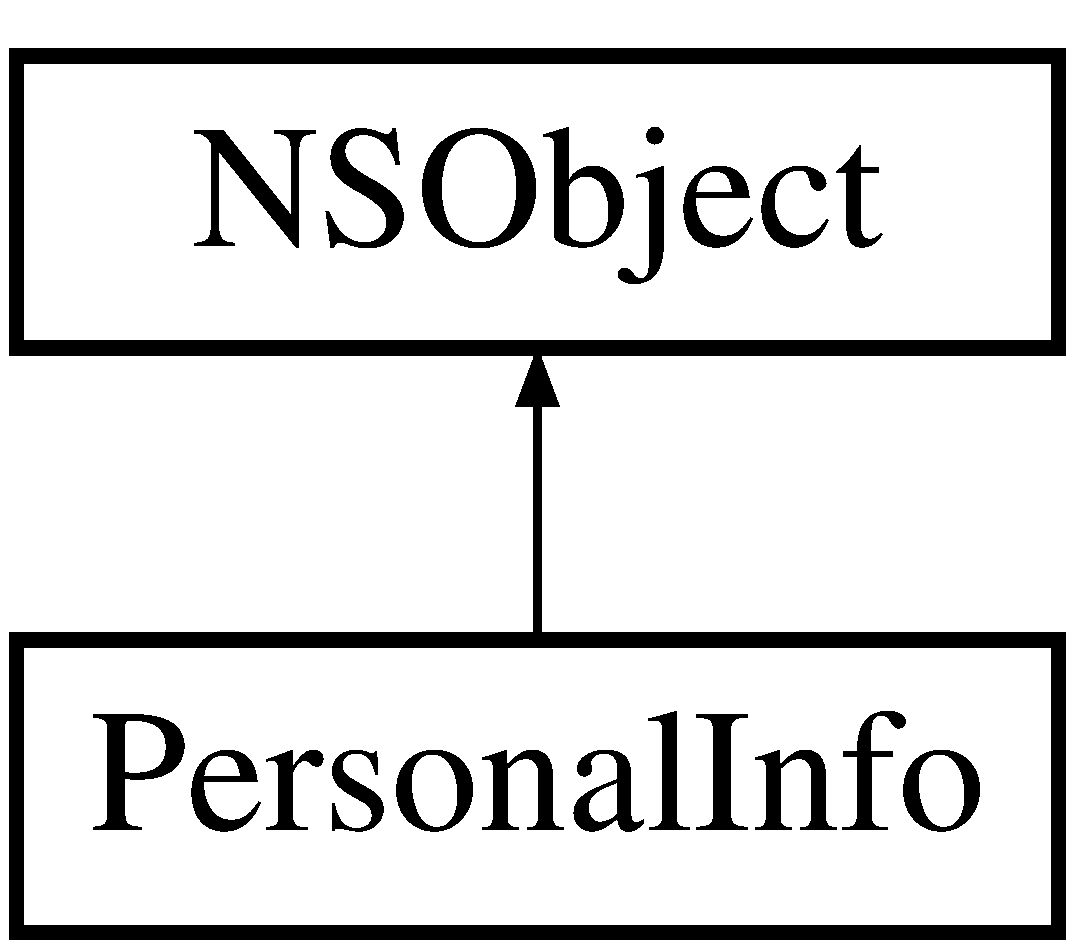
\includegraphics[height=2.000000cm]{interface_personal_info}
\end{center}
\end{figure}
\subsection*{Instance Methods}
\begin{DoxyCompactItemize}
\item 
(void) -\/ \hyperlink{interface_personal_info_a837ce1e3fe6b67a415629e395ce9367e}{load\-Information}
\item 
(void) -\/ \hyperlink{interface_personal_info_a74efb2fadb7b9358f743830b49755567}{save\-Information}
\item 
(void) -\/ \hyperlink{interface_personal_info_ae2b7828f42d1577ed2200b05ceafff26}{dealloc}
\item 
(N\-S\-Integer) -\/ \hyperlink{interface_personal_info_a21553b6f3de4bdbd30eded3d18c44b0b}{calculate\-Age\-Using\-Date\-:}
\end{DoxyCompactItemize}
\subsection*{Properties}
\begin{DoxyCompactItemize}
\item 
\hypertarget{interface_personal_info_a121bb1d64f2b72f302dc4ed1d67be9c5}{N\-S\-String $\ast$ {\bfseries first\-Name}}\label{interface_personal_info_a121bb1d64f2b72f302dc4ed1d67be9c5}

\item 
\hypertarget{interface_personal_info_ac22bfdc40d4d2e7364cd9b2e3b690faf}{N\-S\-String $\ast$ {\bfseries last\-Name}}\label{interface_personal_info_ac22bfdc40d4d2e7364cd9b2e3b690faf}

\item 
\hypertarget{interface_personal_info_a4ba682cdc1f6166765925040634eb5e6}{N\-S\-Date $\ast$ {\bfseries dob}}\label{interface_personal_info_a4ba682cdc1f6166765925040634eb5e6}

\item 
\hypertarget{interface_personal_info_a04b3f994e4c8710fa56c64116973e6a7}{N\-S\-Integer {\bfseries patient\-I\-D}}\label{interface_personal_info_a04b3f994e4c8710fa56c64116973e6a7}

\item 
\hypertarget{interface_personal_info_a2d8d93ba28e6ba9f25b703354004bebf}{N\-S\-User\-Defaults $\ast$ {\bfseries defaults}}\label{interface_personal_info_a2d8d93ba28e6ba9f25b703354004bebf}

\item 
\hypertarget{interface_personal_info_a14b1147d252ca7d5701b5531e6073f2c}{N\-S\-Dictionary $\ast$ {\bfseries personal\-Data}}\label{interface_personal_info_a14b1147d252ca7d5701b5531e6073f2c}

\item 
\hypertarget{interface_personal_info_a765c84fac14d1ed3720d06eaee948df0}{N\-S\-Integer {\bfseries age}}\label{interface_personal_info_a765c84fac14d1ed3720d06eaee948df0}

\end{DoxyCompactItemize}


\subsection{Method Documentation}
\hypertarget{interface_personal_info_a21553b6f3de4bdbd30eded3d18c44b0b}{\index{Personal\-Info@{Personal\-Info}!calculate\-Age\-Using\-Date\-:@{calculate\-Age\-Using\-Date\-:}}
\index{calculate\-Age\-Using\-Date\-:@{calculate\-Age\-Using\-Date\-:}!PersonalInfo@{Personal\-Info}}
\subsubsection[{calculate\-Age\-Using\-Date\-:}]{\setlength{\rightskip}{0pt plus 5cm}-\/ (N\-S\-Integer) calculate\-Age\-Using\-Date\-: 
\begin{DoxyParamCaption}
\item[{(N\-S\-Date$\ast$)}]{current\-D\-O\-B}
\end{DoxyParamCaption}
}}\label{interface_personal_info_a21553b6f3de4bdbd30eded3d18c44b0b}
This method calculates the ages using Date\-Components.


\begin{DoxyParams}{Parameters}
{\em current\-D\-O\-B} & Todays date. It is left to allow changes based on what is passed and not just restricted to todays date.\\
\hline
\end{DoxyParams}
\begin{DoxyReturn}{Returns}
An integer value express based on years. 
\end{DoxyReturn}
\hypertarget{interface_personal_info_ae2b7828f42d1577ed2200b05ceafff26}{\index{Personal\-Info@{Personal\-Info}!dealloc@{dealloc}}
\index{dealloc@{dealloc}!PersonalInfo@{Personal\-Info}}
\subsubsection[{dealloc}]{\setlength{\rightskip}{0pt plus 5cm}-\/ (void) dealloc 
\begin{DoxyParamCaption}
{}
\end{DoxyParamCaption}
}}\label{interface_personal_info_ae2b7828f42d1577ed2200b05ceafff26}
This method is called as part of A\-R\-C. It has been added because the data is saved to the user defaults location before the memory is released so that changes are not lost. \hypertarget{interface_personal_info_a837ce1e3fe6b67a415629e395ce9367e}{\index{Personal\-Info@{Personal\-Info}!load\-Information@{load\-Information}}
\index{load\-Information@{load\-Information}!PersonalInfo@{Personal\-Info}}
\subsubsection[{load\-Information}]{\setlength{\rightskip}{0pt plus 5cm}-\/ (void) load\-Information 
\begin{DoxyParamCaption}
{}
\end{DoxyParamCaption}
}}\label{interface_personal_info_a837ce1e3fe6b67a415629e395ce9367e}
Loads all the information from the application user defaults and stores them in local variables for quicker and easier access. \hypertarget{interface_personal_info_a74efb2fadb7b9358f743830b49755567}{\index{Personal\-Info@{Personal\-Info}!save\-Information@{save\-Information}}
\index{save\-Information@{save\-Information}!PersonalInfo@{Personal\-Info}}
\subsubsection[{save\-Information}]{\setlength{\rightskip}{0pt plus 5cm}-\/ (void) save\-Information 
\begin{DoxyParamCaption}
{}
\end{DoxyParamCaption}
}}\label{interface_personal_info_a74efb2fadb7b9358f743830b49755567}
Save all the local variables into the user defaults for the application. 

The documentation for this class was generated from the following files\-:\begin{DoxyCompactItemize}
\item 
/\-Users/douglas/\-Documents/software/\-Senior Project/ios/\-Medical Cyborgs/\-Medical Cyborgs/Personal\-Info.\-h\item 
/\-Users/douglas/\-Documents/software/\-Senior Project/ios/\-Medical Cyborgs/\-Medical Cyborgs/Personal\-Info.\-m\end{DoxyCompactItemize}

\hypertarget{interface_polar_h7}{\section{Polar\-H7 Class Reference}
\label{interface_polar_h7}\index{Polar\-H7@{Polar\-H7}}
}


{\ttfamily \#import $<$Polar\-H7.\-h$>$}

Inheritance diagram for Polar\-H7\-:\begin{figure}[H]
\begin{center}
\leavevmode
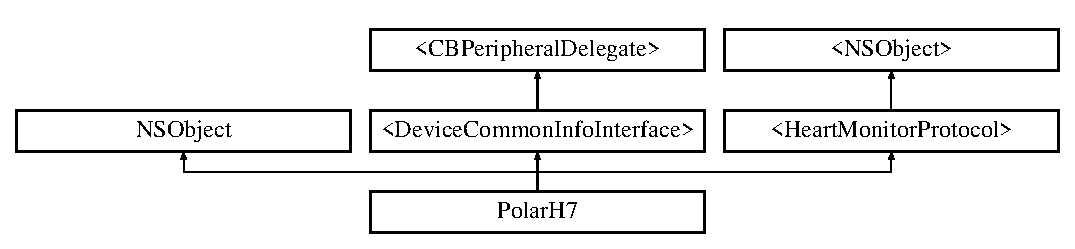
\includegraphics[height=2.901554cm]{interface_polar_h7}
\end{center}
\end{figure}
\subsection*{Properties}
\begin{DoxyCompactItemize}
\item 
\hypertarget{interface_polar_h7_a3819e12cc9802bca0611683cdeaf5775}{N\-S\-Integer {\bfseries type}}\label{interface_polar_h7_a3819e12cc9802bca0611683cdeaf5775}

\item 
\hypertarget{interface_polar_h7_a53721638b179d9373c6a3e17f6ffb3c9}{C\-B\-Service $\ast$ {\bfseries battery\-Service}}\label{interface_polar_h7_a53721638b179d9373c6a3e17f6ffb3c9}

\item 
\hypertarget{interface_polar_h7_a477f7039b2dd7cdcd96519b19cb72581}{C\-B\-Characteristic $\ast$ {\bfseries battery\-Lvl\-Char}}\label{interface_polar_h7_a477f7039b2dd7cdcd96519b19cb72581}

\item 
\hypertarget{interface_polar_h7_a18e69a928d7c29c7db4c6ca05b840064}{C\-B\-Service $\ast$ {\bfseries heart\-Rate\-Service}}\label{interface_polar_h7_a18e69a928d7c29c7db4c6ca05b840064}

\item 
\hypertarget{interface_polar_h7_a64ceb31db248ce9151f0ee1d97d97e6c}{C\-B\-Characteristic $\ast$ {\bfseries heart\-Rate\-Char}}\label{interface_polar_h7_a64ceb31db248ce9151f0ee1d97d97e6c}

\item 
\hypertarget{interface_polar_h7_a333bcccf6282727ccd5e159a66fb6376}{int {\bfseries battery\-Level}}\label{interface_polar_h7_a333bcccf6282727ccd5e159a66fb6376}

\item 
\hypertarget{interface_polar_h7_a8ac64bcce44c2cff369e6edf4e58329d}{C\-B\-Peripheral $\ast$ {\bfseries device}}\label{interface_polar_h7_a8ac64bcce44c2cff369e6edf4e58329d}

\item 
\hypertarget{interface_polar_h7_ad654b125b8f042a6c2407ad4840ac401}{N\-S\-String $\ast$ {\bfseries device\-Manufacturer}}\label{interface_polar_h7_ad654b125b8f042a6c2407ad4840ac401}

\item 
\hypertarget{interface_polar_h7_a1d4ad05750f8373bdf15aad8f9e2cb6d}{N\-S\-Integer {\bfseries current\-Heart\-Rate}}\label{interface_polar_h7_a1d4ad05750f8373bdf15aad8f9e2cb6d}

\end{DoxyCompactItemize}
\subsection*{Additional Inherited Members}


\subsection{Detailed Description}
This class is for the Polar H7 wristband device. Device specific U\-U\-I\-Ds for services and characteristics are here along with the execution path to obtain the desired data for the application. Service and Characteristic U\-U\-I\-Ds are defined in this header instead of gobally in an effort to reduce mental noise when reading the code. The \hyperlink{class_c_b_peripheral_delegate-p}{C\-B\-Peripheral\-Delegate} is implemented so that the class can perform all the operations needed to maintain connection status and retrieval of the data. 

The documentation for this class was generated from the following files\-:\begin{DoxyCompactItemize}
\item 
/\-Users/douglas/\-Documents/software/\-Senior Project/ios/\-Medical Cyborgs/\-Medical Cyborgs/Polar\-H7.\-h\item 
/\-Users/douglas/\-Documents/software/\-Senior Project/ios/\-Medical Cyborgs/\-Medical Cyborgs/Polar\-H7.\-m\end{DoxyCompactItemize}

\hypertarget{interface_remote_d_b_connection_manager}{\section{Remote\-D\-B\-Connection\-Manager Class Reference}
\label{interface_remote_d_b_connection_manager}\index{Remote\-D\-B\-Connection\-Manager@{Remote\-D\-B\-Connection\-Manager}}
}
Inheritance diagram for Remote\-D\-B\-Connection\-Manager\-:\begin{figure}[H]
\begin{center}
\leavevmode
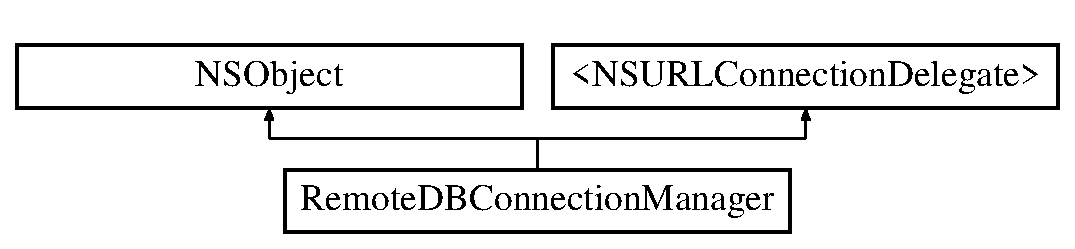
\includegraphics[height=2.000000cm]{interface_remote_d_b_connection_manager}
\end{center}
\end{figure}
\subsection*{Instance Methods}
\begin{DoxyCompactItemize}
\item 
(id) -\/ \hyperlink{interface_remote_d_b_connection_manager_a744cbe8cedf02655ce5a2311957059cb}{init\-With\-Database\-:}
\item 
(void) -\/ \hyperlink{interface_remote_d_b_connection_manager_a517a86ad693e383d664972123808b9fc}{push\-Data\-To\-Remote\-Server}
\item 
(void) -\/ \hyperlink{interface_remote_d_b_connection_manager_aa7263ee167de6993f3c68d74f34d3b9e}{send\-Row\-To\-Server}
\item 
(void) -\/ \hyperlink{interface_remote_d_b_connection_manager_a87140c7af270366183486e2f02dc6f5d}{remove\-Current\-Row\-In\-Local\-D\-B}
\item 
(N\-S\-String $\ast$) -\/ \hyperlink{interface_remote_d_b_connection_manager_a56943f27947c97c9c0d88bf3f89a73f6}{U\-R\-L\-Encoded\-String\-:}
\end{DoxyCompactItemize}
\subsection*{Properties}
\begin{DoxyCompactItemize}
\item 
\hypertarget{interface_remote_d_b_connection_manager_aea31c73a0a3e36095f04688a9b51b594}{\hyperlink{interface_d_b_manager}{D\-B\-Manager} $\ast$ {\bfseries database}}\label{interface_remote_d_b_connection_manager_aea31c73a0a3e36095f04688a9b51b594}

\item 
\hypertarget{interface_remote_d_b_connection_manager_a984d4293c7de824df8ab8b7a8510c15e}{N\-S\-Integer {\bfseries patient\-I\-D}}\label{interface_remote_d_b_connection_manager_a984d4293c7de824df8ab8b7a8510c15e}

\item 
\hypertarget{interface_remote_d_b_connection_manager_a1cf642f7f159dedf3f805ae62f86f0ee}{\hyperlink{interface_local_d_b_result}{Local\-D\-B\-Result} $\ast$ {\bfseries current\-Row}}\label{interface_remote_d_b_connection_manager_a1cf642f7f159dedf3f805ae62f86f0ee}

\item 
\hypertarget{interface_remote_d_b_connection_manager_a6956166be867026a4ed5c9552c2fbc85}{N\-S\-Mutable\-Data $\ast$ {\bfseries \-\_\-server\-Response\-Data}}\label{interface_remote_d_b_connection_manager_a6956166be867026a4ed5c9552c2fbc85}

\item 
\hypertarget{interface_remote_d_b_connection_manager_aea06d1743882f6b59247e590cdd0513f}{N\-S\-Integer {\bfseries failed\-Attempts}}\label{interface_remote_d_b_connection_manager_aea06d1743882f6b59247e590cdd0513f}

\item 
\hypertarget{interface_remote_d_b_connection_manager_ad3cb931f4c5147c3595679f241a0bf48}{B\-O\-O\-L {\bfseries remote\-Unreachable}}\label{interface_remote_d_b_connection_manager_ad3cb931f4c5147c3595679f241a0bf48}

\end{DoxyCompactItemize}


\subsection{Method Documentation}
\hypertarget{interface_remote_d_b_connection_manager_a744cbe8cedf02655ce5a2311957059cb}{\index{Remote\-D\-B\-Connection\-Manager@{Remote\-D\-B\-Connection\-Manager}!init\-With\-Database\-:@{init\-With\-Database\-:}}
\index{init\-With\-Database\-:@{init\-With\-Database\-:}!RemoteDBConnectionManager@{Remote\-D\-B\-Connection\-Manager}}
\subsubsection[{init\-With\-Database\-:}]{\setlength{\rightskip}{0pt plus 5cm}-\/ (id) init\-With\-Database\-: 
\begin{DoxyParamCaption}
\item[{({\bf D\-B\-Manager}$\ast$)}]{datastore}
\end{DoxyParamCaption}
}}\label{interface_remote_d_b_connection_manager_a744cbe8cedf02655ce5a2311957059cb}
This method creates an instance using the database manager that is passed to it. This is the preferred method. If no database is given it will attempt to to open the database and assign it.


\begin{DoxyParams}{Parameters}
{\em datastore} & The database manager that is to be the source of data to send to the server.\\
\hline
\end{DoxyParams}
\begin{DoxyReturn}{Returns}
An instance of the remote server manager. 
\end{DoxyReturn}
\hypertarget{interface_remote_d_b_connection_manager_a517a86ad693e383d664972123808b9fc}{\index{Remote\-D\-B\-Connection\-Manager@{Remote\-D\-B\-Connection\-Manager}!push\-Data\-To\-Remote\-Server@{push\-Data\-To\-Remote\-Server}}
\index{push\-Data\-To\-Remote\-Server@{push\-Data\-To\-Remote\-Server}!RemoteDBConnectionManager@{Remote\-D\-B\-Connection\-Manager}}
\subsubsection[{push\-Data\-To\-Remote\-Server}]{\setlength{\rightskip}{0pt plus 5cm}-\/ (void) push\-Data\-To\-Remote\-Server 
\begin{DoxyParamCaption}
{}
\end{DoxyParamCaption}
}}\label{interface_remote_d_b_connection_manager_a517a86ad693e383d664972123808b9fc}
This method is the wrapper method for the class. It checks to see if the remote is still reachable and that there is something to send to the server. If the server has been unreachable it ends. If the server is reachable and the database is empty it ends, otherwise it continues going through the database and pushing. \hypertarget{interface_remote_d_b_connection_manager_a87140c7af270366183486e2f02dc6f5d}{\index{Remote\-D\-B\-Connection\-Manager@{Remote\-D\-B\-Connection\-Manager}!remove\-Current\-Row\-In\-Local\-D\-B@{remove\-Current\-Row\-In\-Local\-D\-B}}
\index{remove\-Current\-Row\-In\-Local\-D\-B@{remove\-Current\-Row\-In\-Local\-D\-B}!RemoteDBConnectionManager@{Remote\-D\-B\-Connection\-Manager}}
\subsubsection[{remove\-Current\-Row\-In\-Local\-D\-B}]{\setlength{\rightskip}{0pt plus 5cm}-\/ (void) remove\-Current\-Row\-In\-Local\-D\-B 
\begin{DoxyParamCaption}
{}
\end{DoxyParamCaption}
}}\label{interface_remote_d_b_connection_manager_a87140c7af270366183486e2f02dc6f5d}
This method removes the current row from the database. It is called after a successful push to the remote server. For our purposes, the local database essentially functions as a queue with an additional save state. In case of application crash or phone crash, etc the data is not lost and seemed easier to implement than a persistent data store. \hypertarget{interface_remote_d_b_connection_manager_aa7263ee167de6993f3c68d74f34d3b9e}{\index{Remote\-D\-B\-Connection\-Manager@{Remote\-D\-B\-Connection\-Manager}!send\-Row\-To\-Server@{send\-Row\-To\-Server}}
\index{send\-Row\-To\-Server@{send\-Row\-To\-Server}!RemoteDBConnectionManager@{Remote\-D\-B\-Connection\-Manager}}
\subsubsection[{send\-Row\-To\-Server}]{\setlength{\rightskip}{0pt plus 5cm}-\/ (void) send\-Row\-To\-Server 
\begin{DoxyParamCaption}
{}
\end{DoxyParamCaption}
}}\label{interface_remote_d_b_connection_manager_aa7263ee167de6993f3c68d74f34d3b9e}
This method is the workhorse of the class. It retrieves the first first row from the database. Then it creates a U\-R\-L based on the data it retrieved. Then it makes a U\-R\-L request to the server. After that the N\-S\-U\-R\-L\-Connection delete methods handle the calls and continue the loop. \hypertarget{interface_remote_d_b_connection_manager_a56943f27947c97c9c0d88bf3f89a73f6}{\index{Remote\-D\-B\-Connection\-Manager@{Remote\-D\-B\-Connection\-Manager}!U\-R\-L\-Encoded\-String\-:@{U\-R\-L\-Encoded\-String\-:}}
\index{U\-R\-L\-Encoded\-String\-:@{U\-R\-L\-Encoded\-String\-:}!RemoteDBConnectionManager@{Remote\-D\-B\-Connection\-Manager}}
\subsubsection[{U\-R\-L\-Encoded\-String\-:}]{\setlength{\rightskip}{0pt plus 5cm}-\/ (N\-S\-String $\ast$) U\-R\-L\-Encoded\-String\-: 
\begin{DoxyParamCaption}
\item[{(N\-S\-String$\ast$)}]{utf\-String}
\end{DoxyParamCaption}
}}\label{interface_remote_d_b_connection_manager_a56943f27947c97c9c0d88bf3f89a73f6}
This is probably a bad hack. This method is used to encode the string into a U\-R\-L suitable for the server. It does not escape the ? = \& \-\_\- -\/ / symbols. It has been put into place because the default apple method for url encoding a string with encoding does not encode \-:'s. Unfortunately the datetime response from the local database includes colons. Using the search and replace method appears to has some undefined behavior and places extra escape sequences where none are wanted or needed.


\begin{DoxyParams}{Parameters}
{\em utf\-String} & The incoming string that will be utf8 encoded and then converted to a U\-R\-L.\\
\hline
\end{DoxyParams}
\begin{DoxyReturn}{Returns}
A N\-S\-String that is a new U\-R\-L with \% encoding. 
\end{DoxyReturn}


The documentation for this class was generated from the following files\-:\begin{DoxyCompactItemize}
\item 
Remote\-D\-B\-Connection\-Manager.\-h\item 
Remote\-D\-B\-Connection\-Manager.\-m\end{DoxyCompactItemize}

\hypertarget{interface_table_v_c_with_sounds}{\section{Table\-V\-C\-With\-Sounds Class Reference}
\label{interface_table_v_c_with_sounds}\index{Table\-V\-C\-With\-Sounds@{Table\-V\-C\-With\-Sounds}}
}


{\ttfamily \#import $<$Table\-V\-C\-With\-Sounds.\-h$>$}

Inheritance diagram for Table\-V\-C\-With\-Sounds\-:\begin{figure}[H]
\begin{center}
\leavevmode
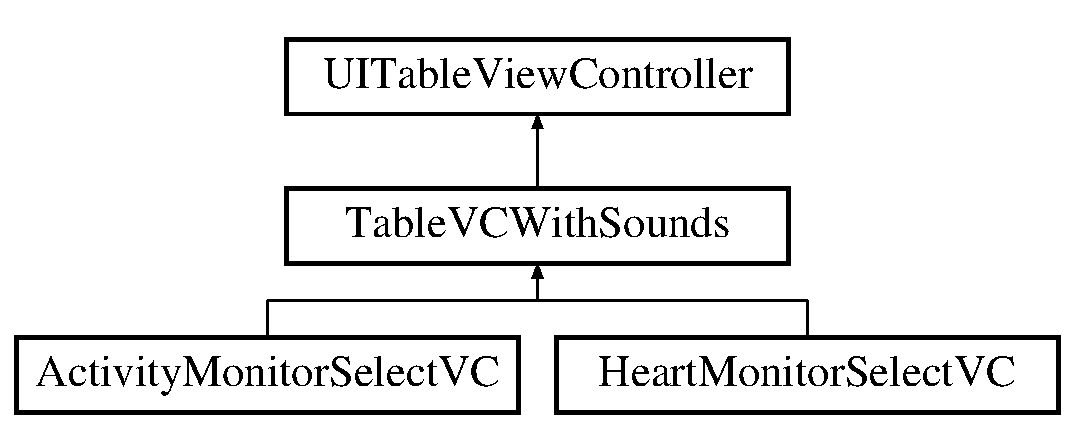
\includegraphics[height=3.000000cm]{interface_table_v_c_with_sounds}
\end{center}
\end{figure}
\subsection*{Instance Methods}
\begin{DoxyCompactItemize}
\item 
(void) -\/ \hyperlink{interface_table_v_c_with_sounds_ad6f4138cb1ce20398ff2b004a1d72143}{play\-View\-Change\-Sound}
\item 
(void) -\/ \hyperlink{interface_table_v_c_with_sounds_abca3853865cb3bc0baf5a12b6f6e3a47}{play\-Click\-Sound}
\item 
(void) -\/ \hyperlink{interface_table_v_c_with_sounds_ab472120173deceba269ec2acd946bbf7}{play\-Sound\-With\-File\-:}
\item 
(id) -\/ \hyperlink{interface_table_v_c_with_sounds_adc0912c1502c5b3e18871081eb87e732}{init\-With\-Device\-Manager\-:}
\item 
(void) -\/ \hyperlink{interface_table_v_c_with_sounds_a95ae2a39d8d064c192e3d608dbc8f275}{update\-Table\-:}
\end{DoxyCompactItemize}
\subsection*{Properties}
\begin{DoxyCompactItemize}
\item 
\hypertarget{interface_table_v_c_with_sounds_a1d5a3b65dc2d25613e6b3ee5e3eeec22}{A\-V\-Audio\-Player $\ast$ {\bfseries sound\-Player}}\label{interface_table_v_c_with_sounds_a1d5a3b65dc2d25613e6b3ee5e3eeec22}

\item 
\hypertarget{interface_table_v_c_with_sounds_a54320e7404010ce9fcdc14ec1f065091}{\hyperlink{interface_b_t_device_manager}{B\-T\-Device\-Manager} $\ast$ {\bfseries device\-Manager}}\label{interface_table_v_c_with_sounds_a54320e7404010ce9fcdc14ec1f065091}

\end{DoxyCompactItemize}


\subsection{Detailed Description}
This base class is a viewcontroller with sound implementation. It allows clicking sounds when a device is selected. 

\subsection{Method Documentation}
\hypertarget{interface_table_v_c_with_sounds_adc0912c1502c5b3e18871081eb87e732}{\index{Table\-V\-C\-With\-Sounds@{Table\-V\-C\-With\-Sounds}!init\-With\-Device\-Manager\-:@{init\-With\-Device\-Manager\-:}}
\index{init\-With\-Device\-Manager\-:@{init\-With\-Device\-Manager\-:}!TableVCWithSounds@{Table\-V\-C\-With\-Sounds}}
\subsubsection[{init\-With\-Device\-Manager\-:}]{\setlength{\rightskip}{0pt plus 5cm}-\/ (id) init\-With\-Device\-Manager\-: 
\begin{DoxyParamCaption}
\item[{({\bf B\-T\-Device\-Manager}$\ast$)}]{new\-Device\-Manager}
\end{DoxyParamCaption}
}}\label{interface_table_v_c_with_sounds_adc0912c1502c5b3e18871081eb87e732}
Creates a device selection view controller. The purpose of the method is to create a standard initialization process for the subclasses of this class. All of the subclasses require a bluetooth device manager and need to be active to start building the view. The \hyperlink{interface_b_t_device_manager}{B\-T\-Device\-Manager} functions as the datasource for this tableviewcontroller and all the subclasses.


\begin{DoxyParams}{Parameters}
{\em new\-Device\-Manager} & the bluetooth device manager that will serve as the data source. \\
\hline
\end{DoxyParams}
\begin{DoxyReturn}{Returns}
Returns a view controller unless no device manager is given, then the result is nil. 
\end{DoxyReturn}
\hypertarget{interface_table_v_c_with_sounds_abca3853865cb3bc0baf5a12b6f6e3a47}{\index{Table\-V\-C\-With\-Sounds@{Table\-V\-C\-With\-Sounds}!play\-Click\-Sound@{play\-Click\-Sound}}
\index{play\-Click\-Sound@{play\-Click\-Sound}!TableVCWithSounds@{Table\-V\-C\-With\-Sounds}}
\subsubsection[{play\-Click\-Sound}]{\setlength{\rightskip}{0pt plus 5cm}-\/ (void) play\-Click\-Sound 
\begin{DoxyParamCaption}
{}
\end{DoxyParamCaption}
}}\label{interface_table_v_c_with_sounds_abca3853865cb3bc0baf5a12b6f6e3a47}
This method is used to sound the audio cue that the monitoring button has been selected. \hypertarget{interface_table_v_c_with_sounds_ab472120173deceba269ec2acd946bbf7}{\index{Table\-V\-C\-With\-Sounds@{Table\-V\-C\-With\-Sounds}!play\-Sound\-With\-File\-:@{play\-Sound\-With\-File\-:}}
\index{play\-Sound\-With\-File\-:@{play\-Sound\-With\-File\-:}!TableVCWithSounds@{Table\-V\-C\-With\-Sounds}}
\subsubsection[{play\-Sound\-With\-File\-:}]{\setlength{\rightskip}{0pt plus 5cm}-\/ (void) play\-Sound\-With\-File\-: 
\begin{DoxyParamCaption}
\item[{(N\-S\-U\-R\-L$\ast$)}]{sound\-File}
\end{DoxyParamCaption}
}}\label{interface_table_v_c_with_sounds_ab472120173deceba269ec2acd946bbf7}
This method is the base method that the others use for playing the audio file. It does the setup of the audio player and uses the file passed to it for playback. 
\begin{DoxyParams}{Parameters}
{\em sound\-File} & The N\-S\-U\-R\-L of the file to be played. \\
\hline
\end{DoxyParams}
\hypertarget{interface_table_v_c_with_sounds_ad6f4138cb1ce20398ff2b004a1d72143}{\index{Table\-V\-C\-With\-Sounds@{Table\-V\-C\-With\-Sounds}!play\-View\-Change\-Sound@{play\-View\-Change\-Sound}}
\index{play\-View\-Change\-Sound@{play\-View\-Change\-Sound}!TableVCWithSounds@{Table\-V\-C\-With\-Sounds}}
\subsubsection[{play\-View\-Change\-Sound}]{\setlength{\rightskip}{0pt plus 5cm}-\/ (void) play\-View\-Change\-Sound 
\begin{DoxyParamCaption}
{}
\end{DoxyParamCaption}
}}\label{interface_table_v_c_with_sounds_ad6f4138cb1ce20398ff2b004a1d72143}
This method is used for audio cue that a view is about to be displayed. \hypertarget{interface_table_v_c_with_sounds_a95ae2a39d8d064c192e3d608dbc8f275}{\index{Table\-V\-C\-With\-Sounds@{Table\-V\-C\-With\-Sounds}!update\-Table\-:@{update\-Table\-:}}
\index{update\-Table\-:@{update\-Table\-:}!TableVCWithSounds@{Table\-V\-C\-With\-Sounds}}
\subsubsection[{update\-Table\-:}]{\setlength{\rightskip}{0pt plus 5cm}-\/ (void) update\-Table\-: 
\begin{DoxyParamCaption}
\item[{(N\-S\-Notification$\ast$)}]{notification}
\end{DoxyParamCaption}
}}\label{interface_table_v_c_with_sounds_a95ae2a39d8d064c192e3d608dbc8f275}
This function is the default method that is called when the device manager discovers a device. Its intent is to allow the tableview to update since the count of devices has changed and information is available. A table reload is used because the number of items to be discovered is very small and the overhead is small. Otherwise it is recommended to just reload the section and choose the type of animation.


\begin{DoxyParams}{Parameters}
{\em notification} & A N\-S\-Notification object, not used at this time. \\
\hline
\end{DoxyParams}


The documentation for this class was generated from the following files\-:\begin{DoxyCompactItemize}
\item 
/\-Users/douglas/\-Documents/software/\-Senior Project/ios/\-Medical Cyborgs/\-Medical Cyborgs/Table\-V\-C\-With\-Sounds.\-h\item 
/\-Users/douglas/\-Documents/software/\-Senior Project/ios/\-Medical Cyborgs/\-Medical Cyborgs/Table\-V\-C\-With\-Sounds.\-m\end{DoxyCompactItemize}

\hypertarget{category_table_v_c_with_sounds_07_08}{\section{Table\-V\-C\-With\-Sounds() Category Reference}
\label{category_table_v_c_with_sounds_07_08}\index{Table\-V\-C\-With\-Sounds()@{Table\-V\-C\-With\-Sounds()}}
}


The documentation for this category was generated from the following file\-:\begin{DoxyCompactItemize}
\item 
Table\-V\-C\-With\-Sounds.\-m\end{DoxyCompactItemize}

\hypertarget{interface_wahoo_tickr_x}{\section{Wahoo\-Tickr\-X Class Reference}
\label{interface_wahoo_tickr_x}\index{Wahoo\-Tickr\-X@{Wahoo\-Tickr\-X}}
}


{\ttfamily \#import $<$Wahoo\-Tickr\-X.\-h$>$}

Inheritance diagram for Wahoo\-Tickr\-X\-:\begin{figure}[H]
\begin{center}
\leavevmode
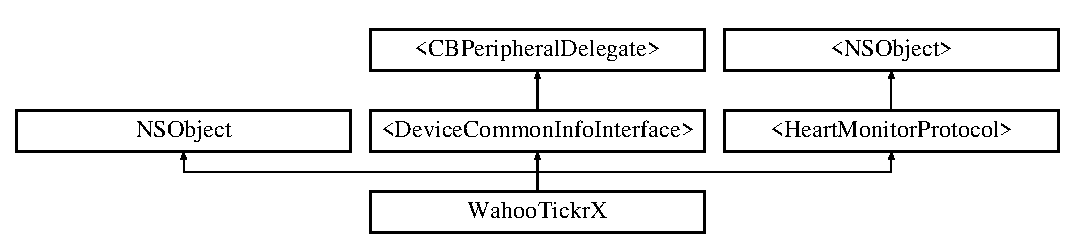
\includegraphics[height=2.901554cm]{interface_wahoo_tickr_x}
\end{center}
\end{figure}
\subsection*{Properties}
\begin{DoxyCompactItemize}
\item 
\hypertarget{interface_wahoo_tickr_x_a96e73fccf071a4f3406e51a833a4756a}{N\-S\-Integer {\bfseries type}}\label{interface_wahoo_tickr_x_a96e73fccf071a4f3406e51a833a4756a}

\item 
\hypertarget{interface_wahoo_tickr_x_a36e3426d855a4cb1ea5495afb7d5818c}{N\-S\-Integer {\bfseries battery\-Level}}\label{interface_wahoo_tickr_x_a36e3426d855a4cb1ea5495afb7d5818c}

\item 
\hypertarget{interface_wahoo_tickr_x_a1150e7cbd797825676de42644f16bb93}{C\-B\-Peripheral $\ast$ {\bfseries device}}\label{interface_wahoo_tickr_x_a1150e7cbd797825676de42644f16bb93}

\item 
\hypertarget{interface_wahoo_tickr_x_a4dc92d682d3e9734886c0356bdb86bbf}{C\-B\-Service $\ast$ {\bfseries battery\-Service}}\label{interface_wahoo_tickr_x_a4dc92d682d3e9734886c0356bdb86bbf}

\item 
\hypertarget{interface_wahoo_tickr_x_a664a0a704cfea55c60ddf4dbcad3bf35}{C\-B\-Characteristic $\ast$ {\bfseries battery\-Lvl\-Char}}\label{interface_wahoo_tickr_x_a664a0a704cfea55c60ddf4dbcad3bf35}

\item 
\hypertarget{interface_wahoo_tickr_x_a83d9f36650e71b239075074c551a0185}{N\-S\-Integer {\bfseries current\-Heart\-Rate}}\label{interface_wahoo_tickr_x_a83d9f36650e71b239075074c551a0185}

\item 
\hypertarget{interface_wahoo_tickr_x_ae712f8d6cd74c8fb0b1093f45e7ee6e3}{C\-B\-Service $\ast$ {\bfseries heart\-Rate\-Service}}\label{interface_wahoo_tickr_x_ae712f8d6cd74c8fb0b1093f45e7ee6e3}

\item 
\hypertarget{interface_wahoo_tickr_x_a8d2500c6e9eb3493393631b3bad7f7e7}{C\-B\-Characteristic $\ast$ {\bfseries heart\-Rate\-Char}}\label{interface_wahoo_tickr_x_a8d2500c6e9eb3493393631b3bad7f7e7}

\end{DoxyCompactItemize}
\subsection*{Additional Inherited Members}


\subsection{Detailed Description}
This class is for the Wahoo Tickr X wristband device. Device specific U\-U\-I\-Ds for services and characteristics are here along with the execution path to obtain the desired data for the application. Service and Characteristic U\-U\-I\-Ds are defined in this header instead of gobally in an effort to reduce mental noise when reading the code. The \hyperlink{class_c_b_peripheral_delegate-p}{C\-B\-Peripheral\-Delegate} is implemented so that the class can perform all the operations needed to maintain connection status and retrieval of the data. 

The documentation for this class was generated from the following files\-:\begin{DoxyCompactItemize}
\item 
Wahoo\-Tickr\-X.\-h\item 
Wahoo\-Tickr\-X.\-m\end{DoxyCompactItemize}

%--- End generated contents ---

% Index
\newpage
\phantomsection
\addcontentsline{toc}{part}{Index}
\printindex

\end{document}
